\documentclass[12pt]{article} 

% Adjust margining to narrow
\usepackage{geometry}
\geometry{a4paper, total={170mm,257mm}, left=20mm, top=20mm}

% Mathematics font
\usepackage{amsfonts}
\usepackage{amsmath}

% Graphics import
\usepackage{graphicx}
\usepackage{subcaption}
\graphicspath{{C:/Users/user/Desktop/KUL - Mstat/Big Data Platforms and Technologies/report/graph}}

% Advanced table
\usepackage{tabularx}
\usepackage{makecell}

% No indentation
\setlength\parindent{0pt}

% Python code
\usepackage[scaled=0.85]{FiraMono}
\usepackage{listings}

\lstset{basicstyle=\ttfamily, keywordstyle=\bfseries}

% Hyperlink
\usepackage{hyperref}
\hypersetup{colorlinks=true, urlcolor=blue}

\usepackage{tikz}
\usetikzlibrary{shapes.geometric, arrows}
% ------------------------------------------------------------------------
% Assignment content
\begin{document}
\begin{titlepage}
	\begin{center}
	\vspace*{1cm}
    
\includegraphics[width=0.4\textwidth]{KUL}\\
	\vspace{2.5cm}
    {\Large Report for Advanced Analytics in Business}
            
    \vspace{1.5cm}

    {\large Ana Maria Giraldo Vargas, r0822450}\\
    \vspace{0.5cm}
    {\large David Badajkov, r0604517}\\
    \vspace{0.5cm}
    {\large Marcela 	Lopez Viveros, r0773141}\\
	\vspace{0.5cm}
	{\large Sonia Rocio 	Socadagui Casas, r0823960}\\
	\vspace{0.5cm}
    {\large Wai Chun Cheung, r0817438}
    \vspace{1.5cm}


       \today
   \end{center}
\end{titlepage}

% ------------------------------------------------------------------------
\newpage
\tableofcontents
\newpage

\section*{Assignment 1}
\addcontentsline{toc}{section}{Assignment 1}


\subsection*{Feature engineering}
\addcontentsline{toc}{subsection}{Feature engineering}

The (training) dataset for Assignment 1 consists of 55,463 observations and 78 features. The number of features. It is easy to observe that there are a lot of missing values and categorical or date features in the dataset. In this section, we would discuss the strategies used in handling such problems. 

\subsubsection*{Missing values}
\addcontentsline{toc}{subsubsection}{Missing values}

As shown in figure 1, there are 55 feature which contain missing values, and 24 out of them contain more than 80\% of missing values. For those features with a high proportion of missing values (more than 50\%), missing values are treated as an extra category. By treating missing values as an extra category called \textit{unknown}, the information of the non-missing entries of those features can be retained and learnt by the model, whereas removal of those features may lead to a loss in information or pattern. For those features with a lower proportion of missing values (less than 50\%), some imputation techniques can be applied to estimate their possible values. Another kind of missing values visualization using \texttt{missingno} is presented in figure 2. 

\begin{figure}[h]
\centering
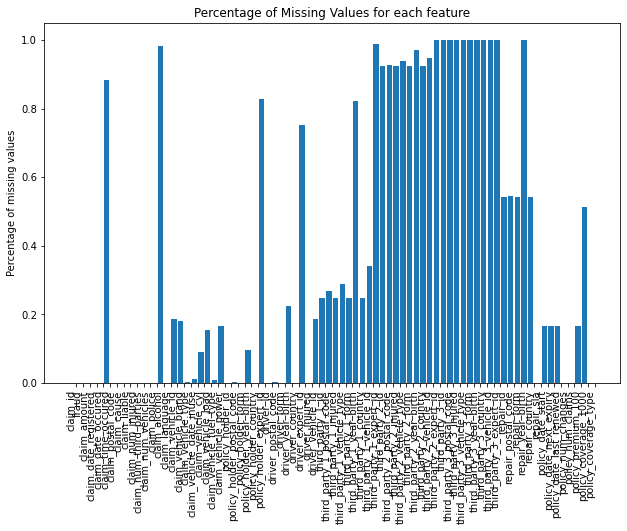
\includegraphics[width=1\linewidth]{missing_value_plt1}
\caption{Proportions of missing values for each feature}
\end{figure}

\begin{figure}[h]
\centering
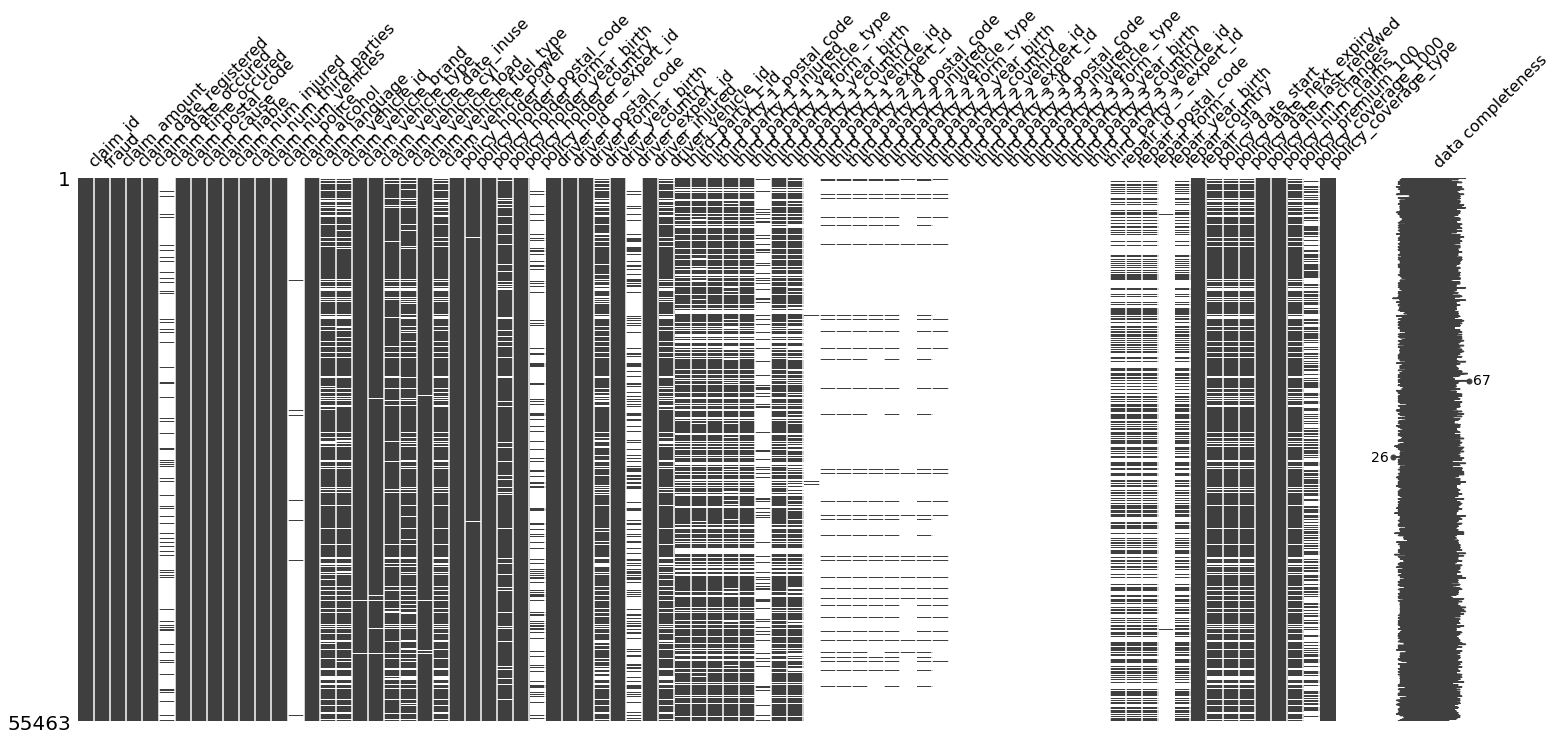
\includegraphics[width=1\linewidth]{missing_value_plt2}
\caption{Visualization of missing values with \texttt{missingno} python library}
\end{figure}

\subsubsection*{Date features}
\addcontentsline{toc}{subsubsection}{Date features}

Some features are available in form of date. In the dataset, the following features are in terms of date: \texttt{claim\_date\_registered}, \texttt{claim\_date\_occured}, \texttt{claim\_vehicle\_date\_inuse}, \texttt{policy\_date\_start}, \texttt{policy\_date\_next\_expiry} and \texttt{policy\_date\_last\_renewed}. However, date itself is not suitable to serve as an input for some machine learning models. Hence, as summarized in table 1, we construct another set of features which are more interpretable and meaningful based on these date features.\\

Apart from the aforementioned features, features related to birth year are also considered as date features. They are \texttt{policy\_holder\_year\_birth}, \texttt{driver\_year\_birth}, \texttt{third\_party\_1\_year\_birth}, \texttt{third\_party\_2\_year\_birth}, \texttt{third\_party\_3\_year\_birth} and \texttt{repair\_year\_birth} in the dataset. By subtracting them from the year of \texttt{claim\_date\_occured}, we obtain age-related features.

\begin{table}[h]
	\begin{tabular}{|l|p{11.5cm}|}
	\hline
	Constructed features & Descriptions\\
	\hline
	\texttt{days\_before\_registered} & The number of days between \texttt{claim\_date\_registered} and \texttt{claim\_date\_occured}.\\
	\hline
	\texttt{days\_before\_occured} & The number of days between \texttt{claim\_date\_occured} and \texttt{claim\_vehicle\_date\_inuse}.\\
	\hline
	\texttt{policy\_length} & The number of days between \texttt{policy\_date\_last\_renewed} and \texttt{policy\_date\_start}.\\
	\hline
	\texttt{policy\_claim\_length} & The number of days between \texttt{policy\_date\_next\_expiry} and \texttt{claim\_date\_occured}.\\
	\hline
	various age-related features & The number of years between the year of \texttt{claim\_date\_occured} and birth year.\\	
	\hline
	\end{tabular}
	\caption{Featurization of date features}
\end{table}

\vspace{-1cm}
\subsubsection*{Data quality issue}
\addcontentsline{toc}{subsubsection}{Data quality issue}

During data cleaning process, we discovered some problems with regards to data quality. For example, the instance with claim id 62780 has an invalid value for the year of \texttt{claim\_vehicle\_date\_\\inuse}. Such observations may be due to input error in manual data entering process. In this case, we may manually correct the year from 2705 to 2005. However, they can be hard and time-consuming to observe in general. A separate data validation process should be carried out before data analysis.

\begin{figure}[h]
\centering
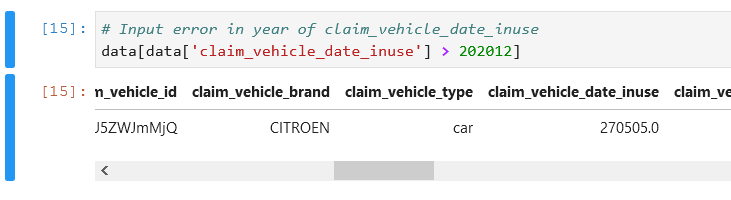
\includegraphics[width=1\linewidth]{data_quality_issue}
\caption{Invalid value of \texttt{claim\_vehicle\_date\_inuse} with claim id 62780}
\end{figure}


\vspace{-1cm}
\subsubsection*{Data binning}
\addcontentsline{toc}{subsubsection}{Data binning}

Binning continuous features can help incorporating missing values and extreme values in a more natural way as they can be reformulated as categorical features. It is useful for those continuous features with a high proportion of missing values or highly right-skewed. For age-related features, they are binned by age groups with equal intervals. In our case, age-related features are encoded into the following categories: $(0, 20], (20, 40], (40, 60], (60, 80], (80, \infty]$ and \textit{unknown}. Equal intervals of 20 years seem to be a reasonable choice by looking at their kernel density estimates of histograms. For driver age and policy holder age, the density looks like bimodal with a local minima around 40 years. Moreover, extreme ages, which are below 20 and above 80, can be handled properly under such binning. 

\begin{figure}[h]
\centering
\begin{subfigure}{.5\textwidth}
  \centering
  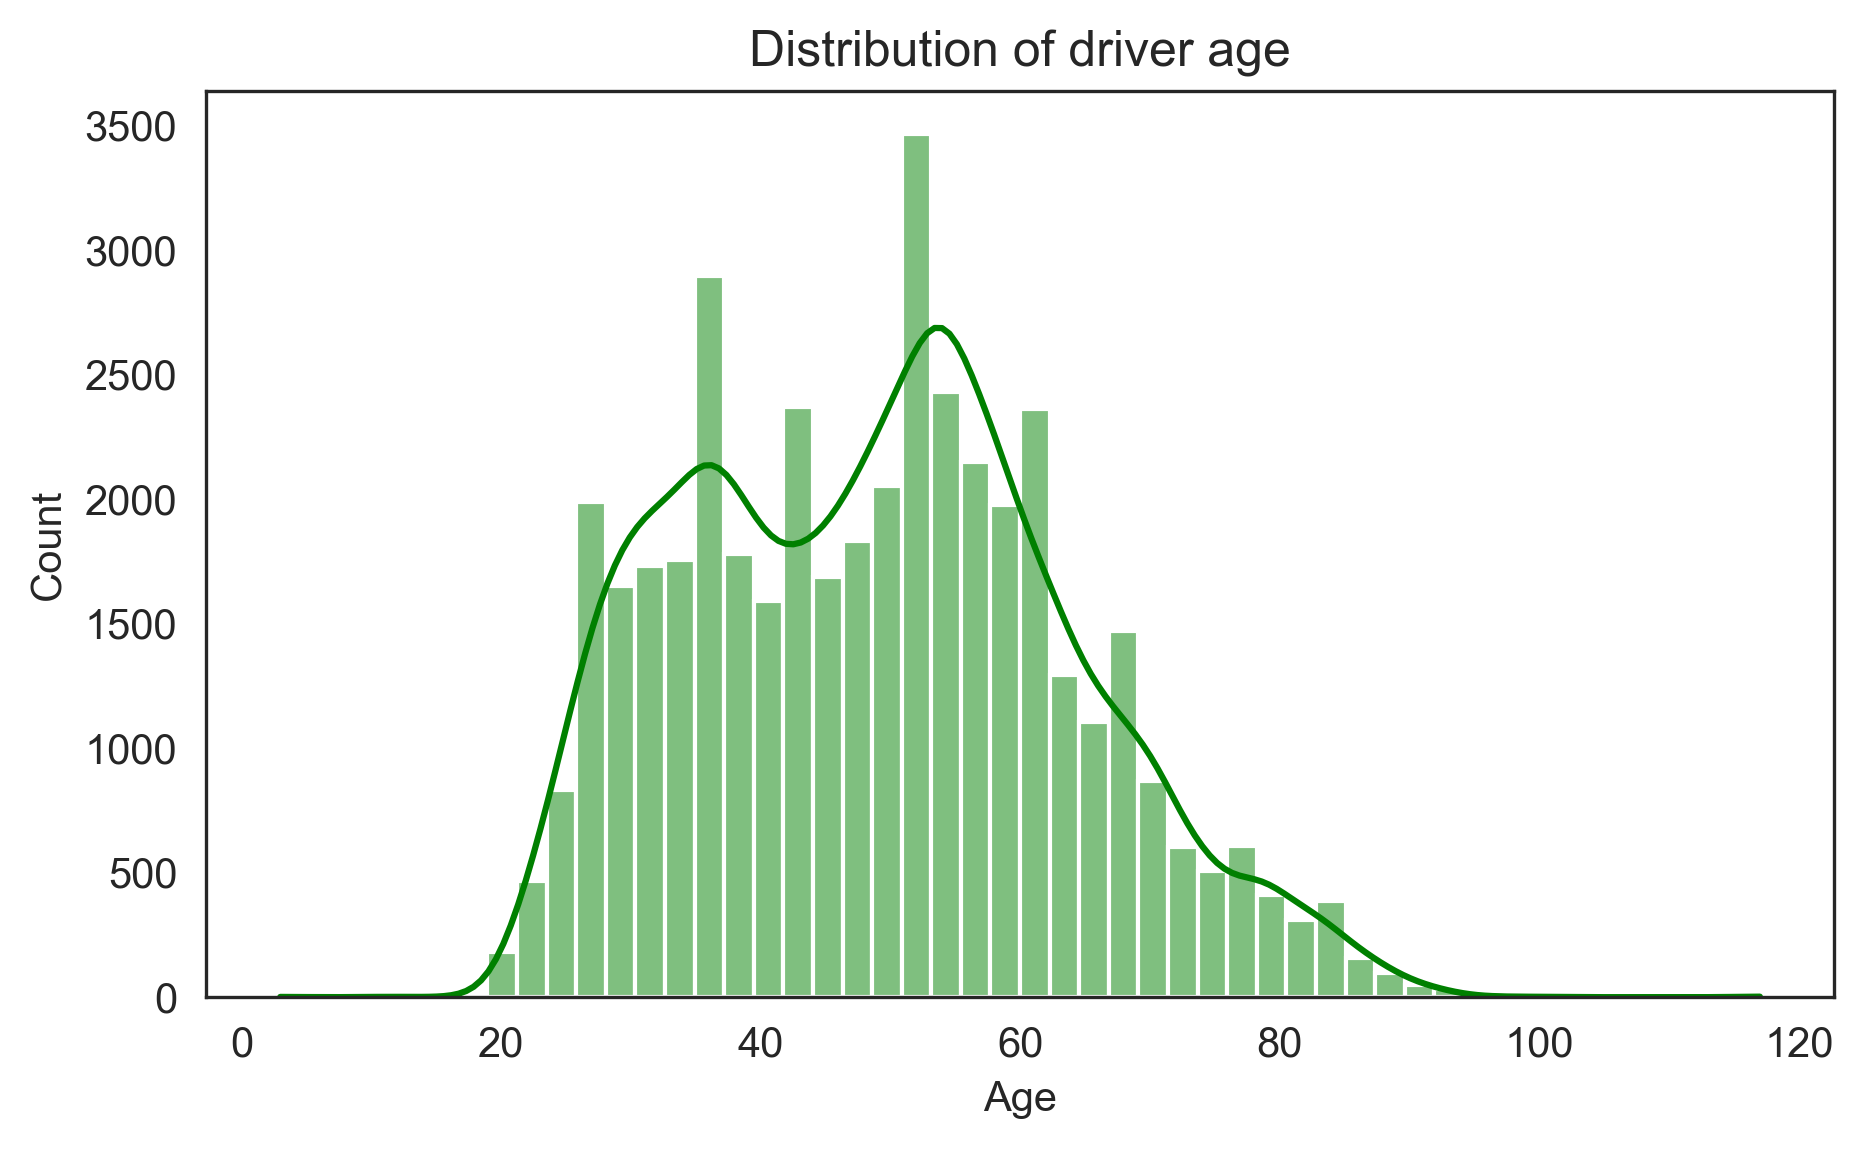
\includegraphics[width=1\linewidth]{dist_driver_age}
  \label{fig:sub1}
\end{subfigure}%
\begin{subfigure}{.5\textwidth}
  \centering
  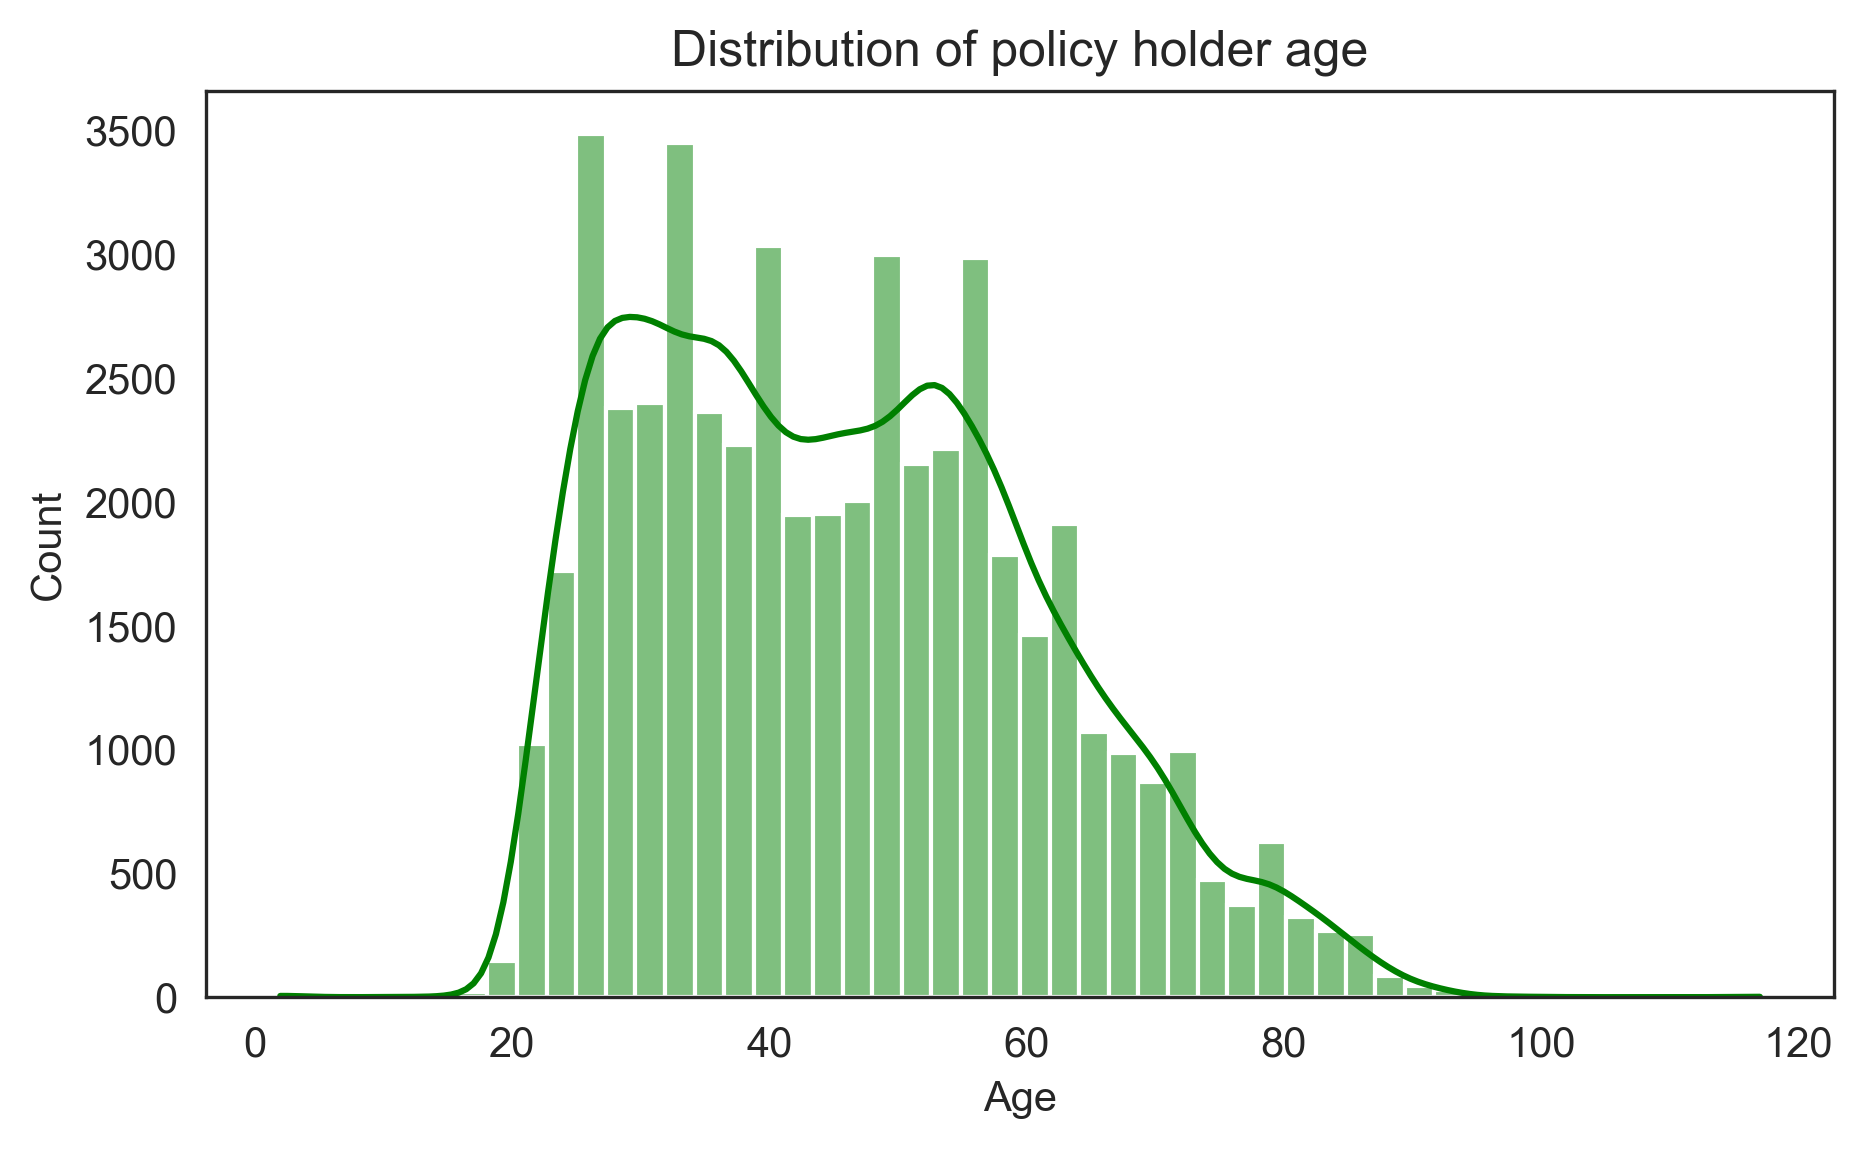
\includegraphics[width=1\linewidth]{dist_policy_holder_age}
  \label{fig:sub2}
\end{subfigure}
\vspace{-1cm}
\begin{subfigure}{.5\textwidth}
  \centering
  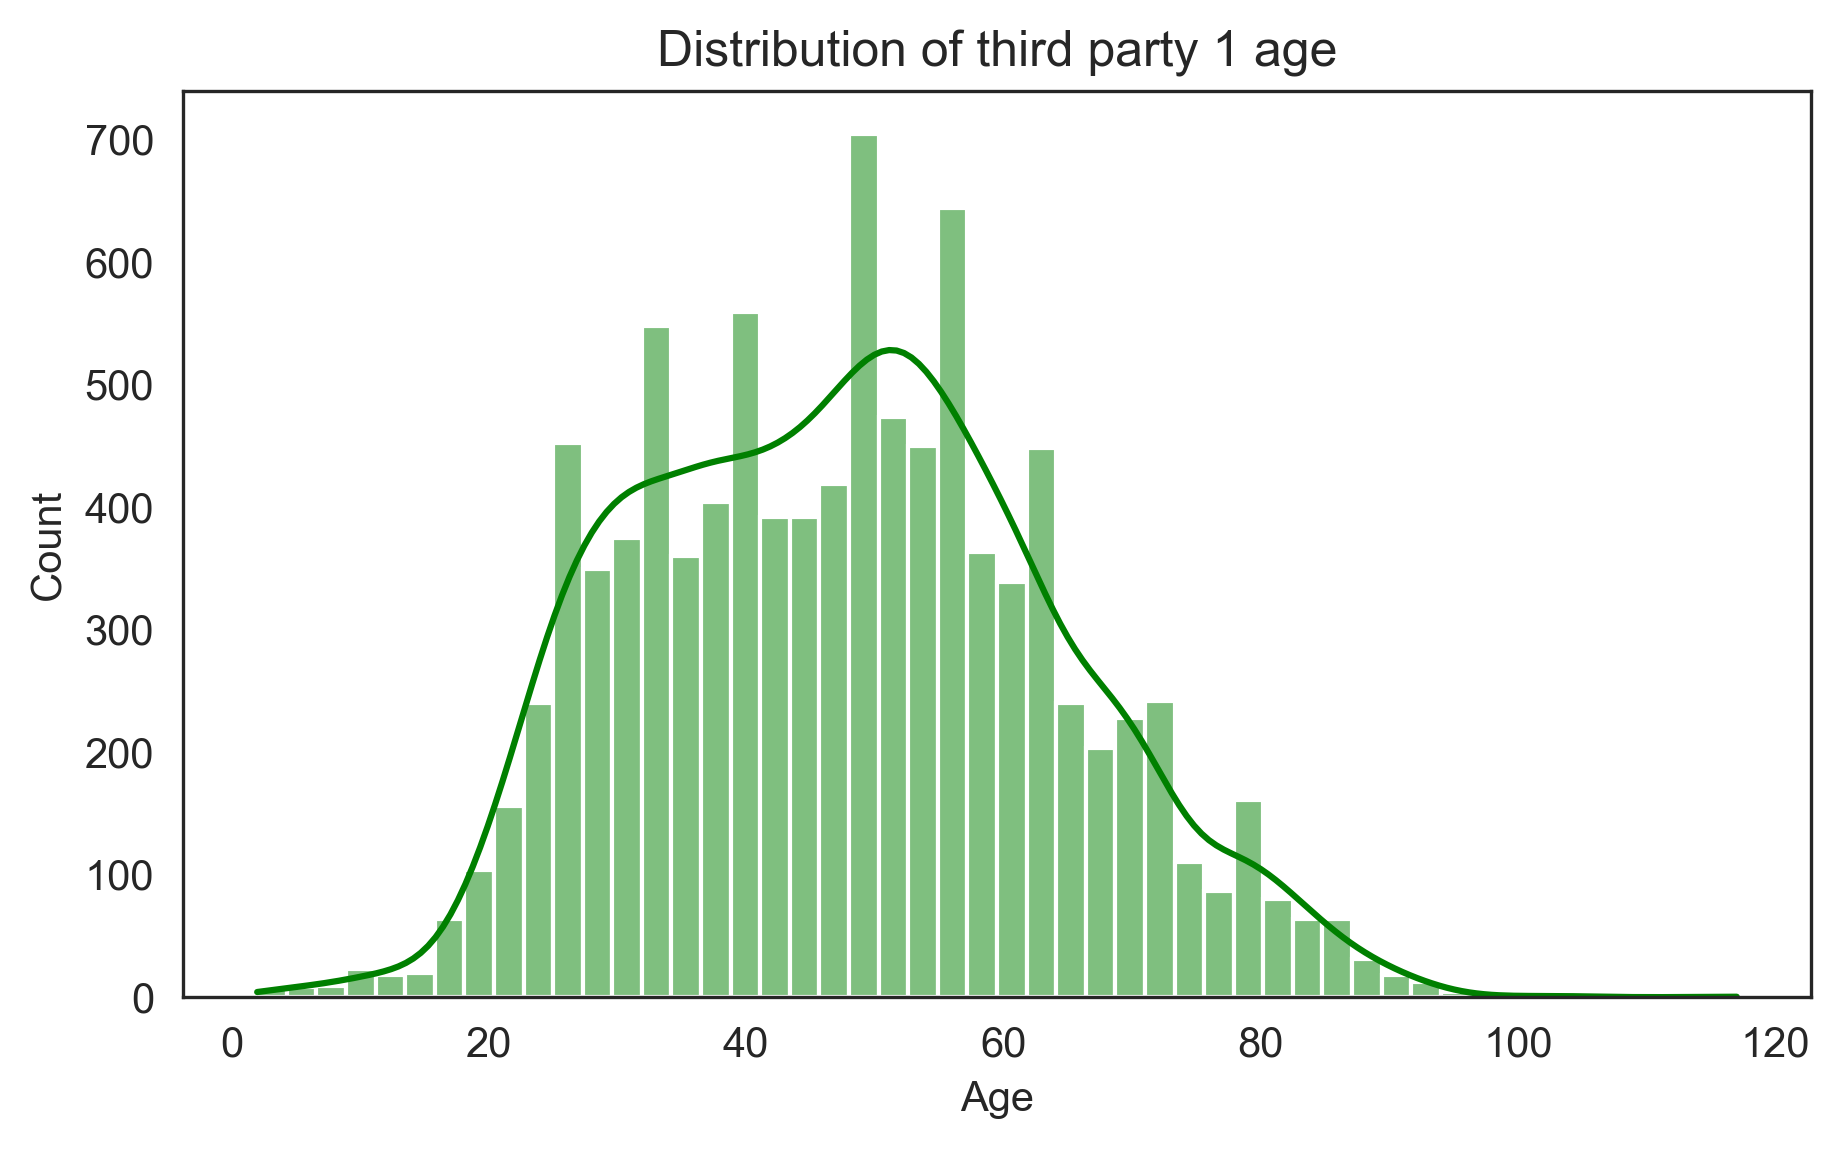
\includegraphics[width=1\linewidth]{dist_third_party_1_age}
  \label{fig:sub3}
\end{subfigure}%
\begin{subfigure}{.5\textwidth}
  \centering
  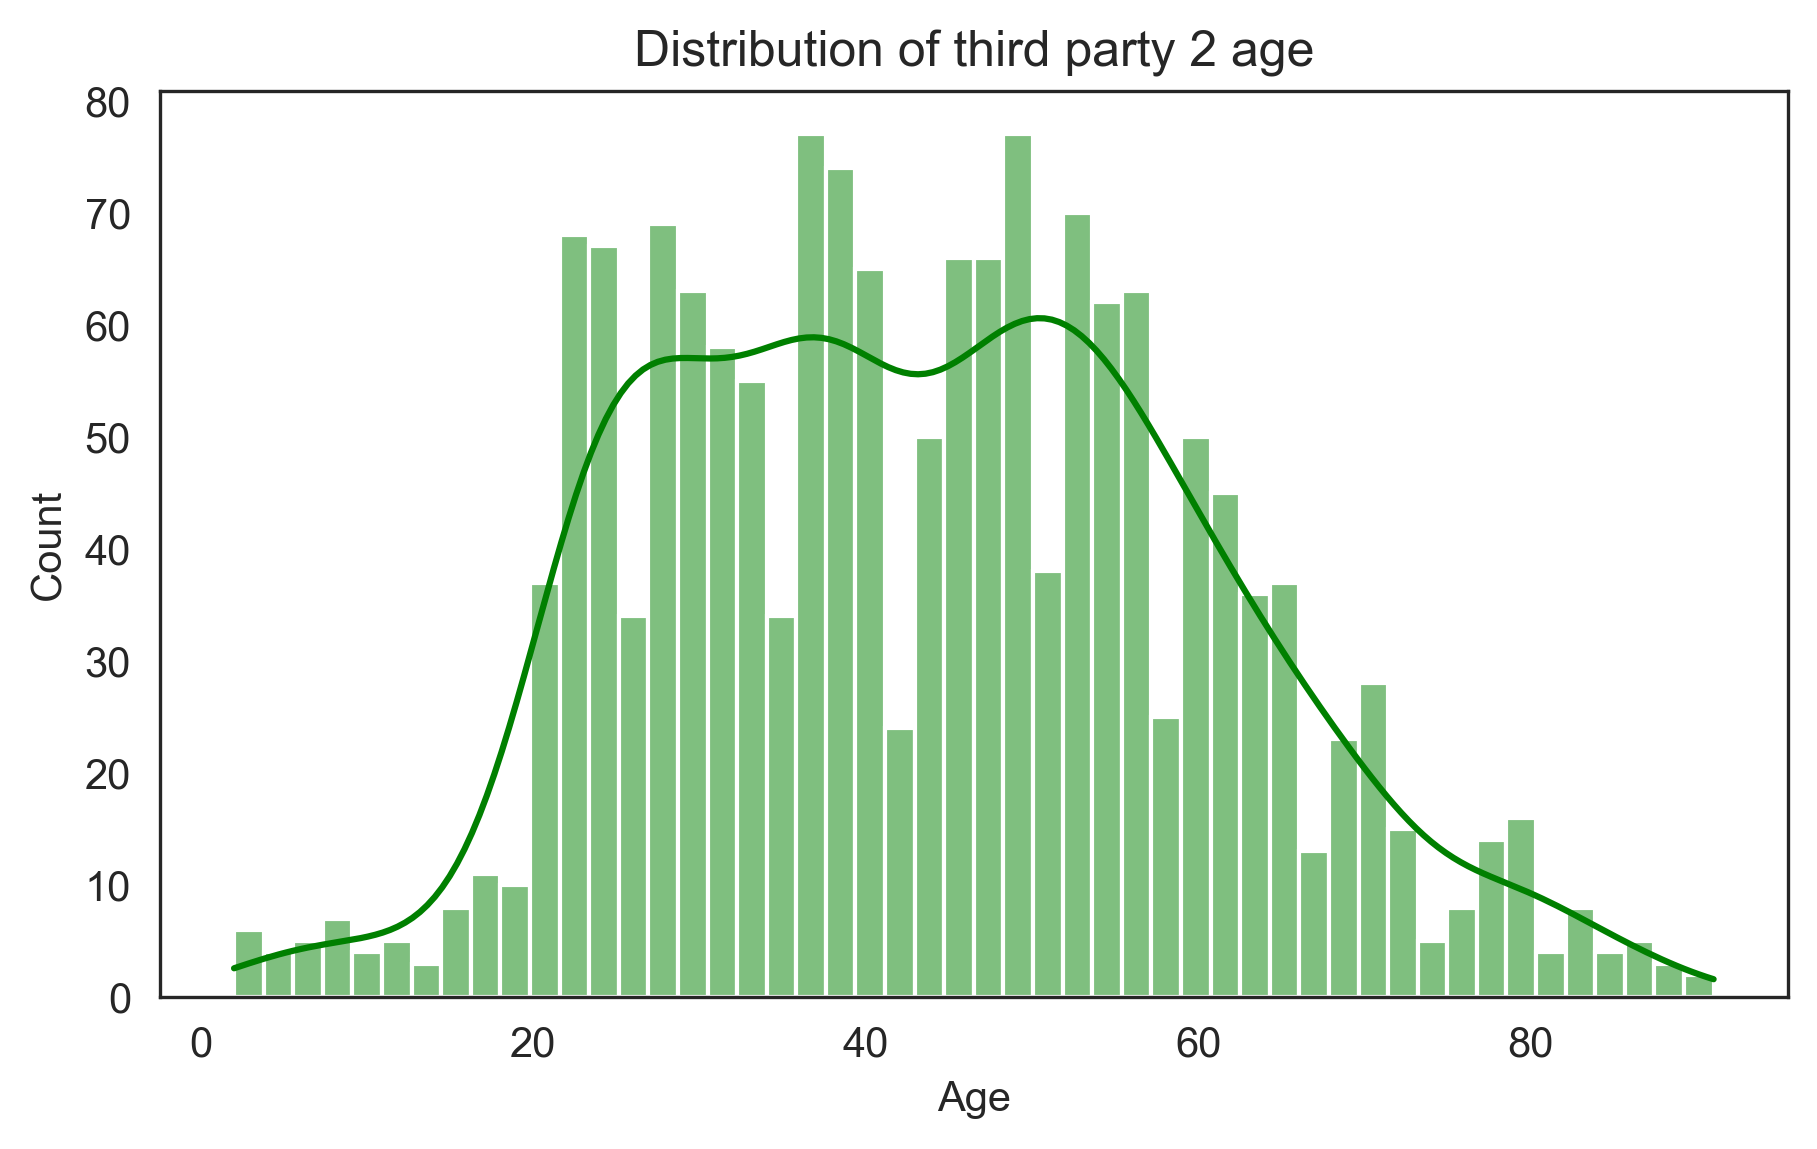
\includegraphics[width=1\linewidth]{dist_third_party_2_age}
  \label{fig:sub4}
\end{subfigure}
\caption{Histograms for age-related features. Green lines are the kernel density estimates. As third party 3 contains only few non-missing values, its histogram is not shown here.}
\label{fig:feature_engineering_age}
\end{figure}

An alternative to kernel density estimate is one-dimensional k-means algorithm. However, k-means algorithm partitions features based on mean and the specified number of clusters $k$. Due to skewness in age-related features, the bin for high age group may be too wide. As shown in figure 5, the fourth group has the range $[63, \infty)$ for \texttt{driver\_age} and \texttt{policy\_holder\_age}. Therefore, we do not apply one dimensional k-means algorithm in this case. 

\begin{figure}[h]
\centering
\begin{subfigure}{.5\textwidth}
  \centering
  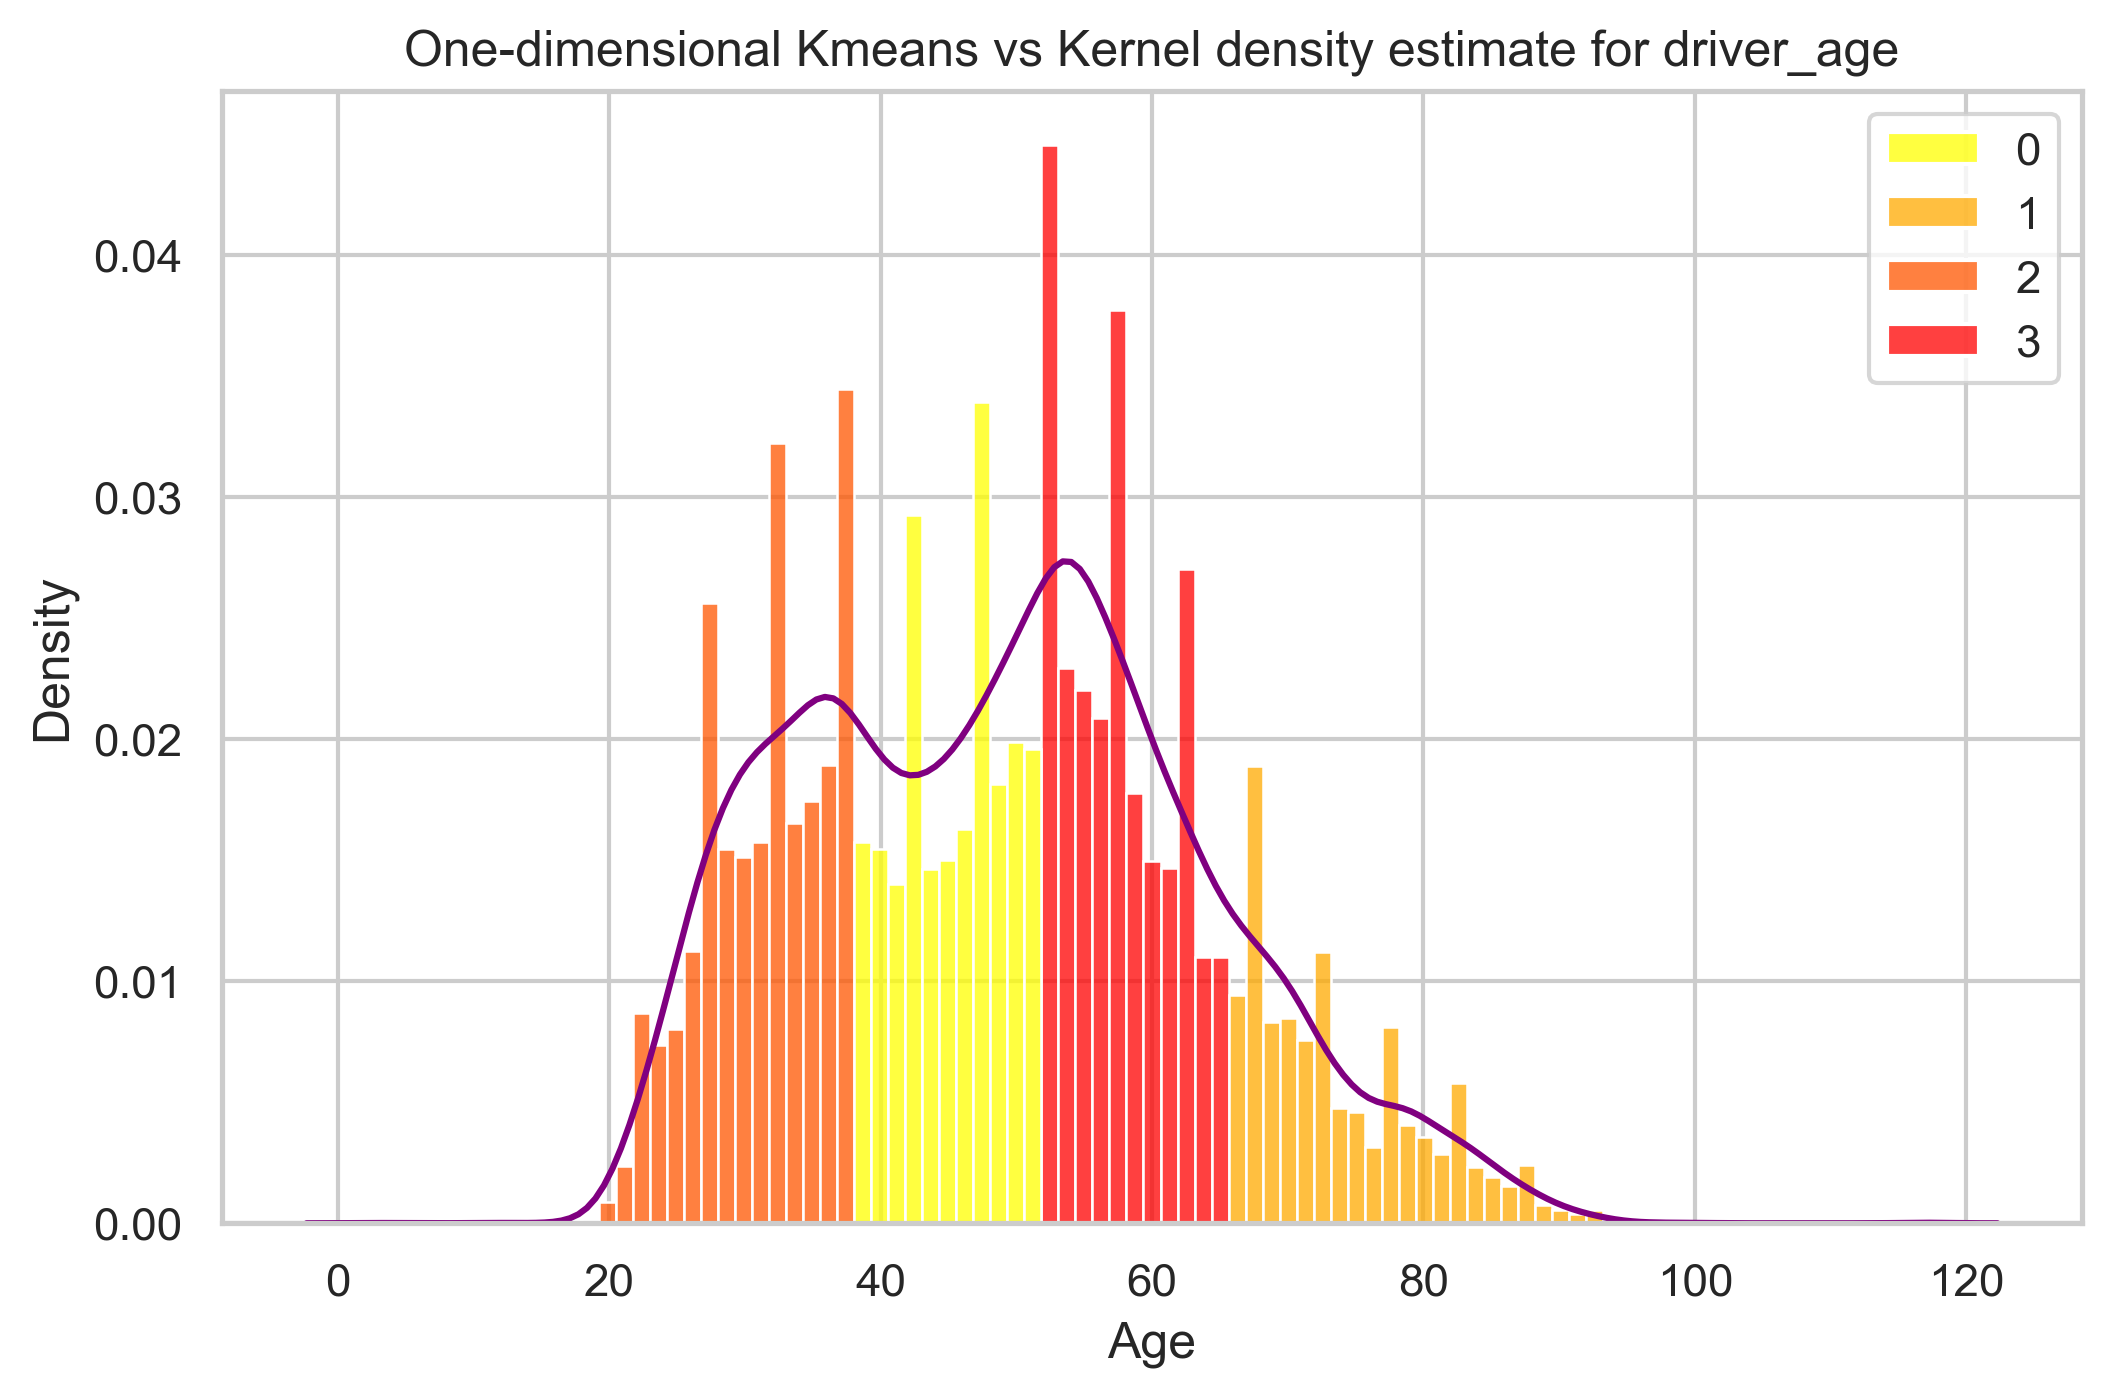
\includegraphics[width=1\linewidth]{one_dim_kmeans}
  \label{fig:sub1}
\end{subfigure}%
\begin{subfigure}{.5\textwidth}
  \centering
  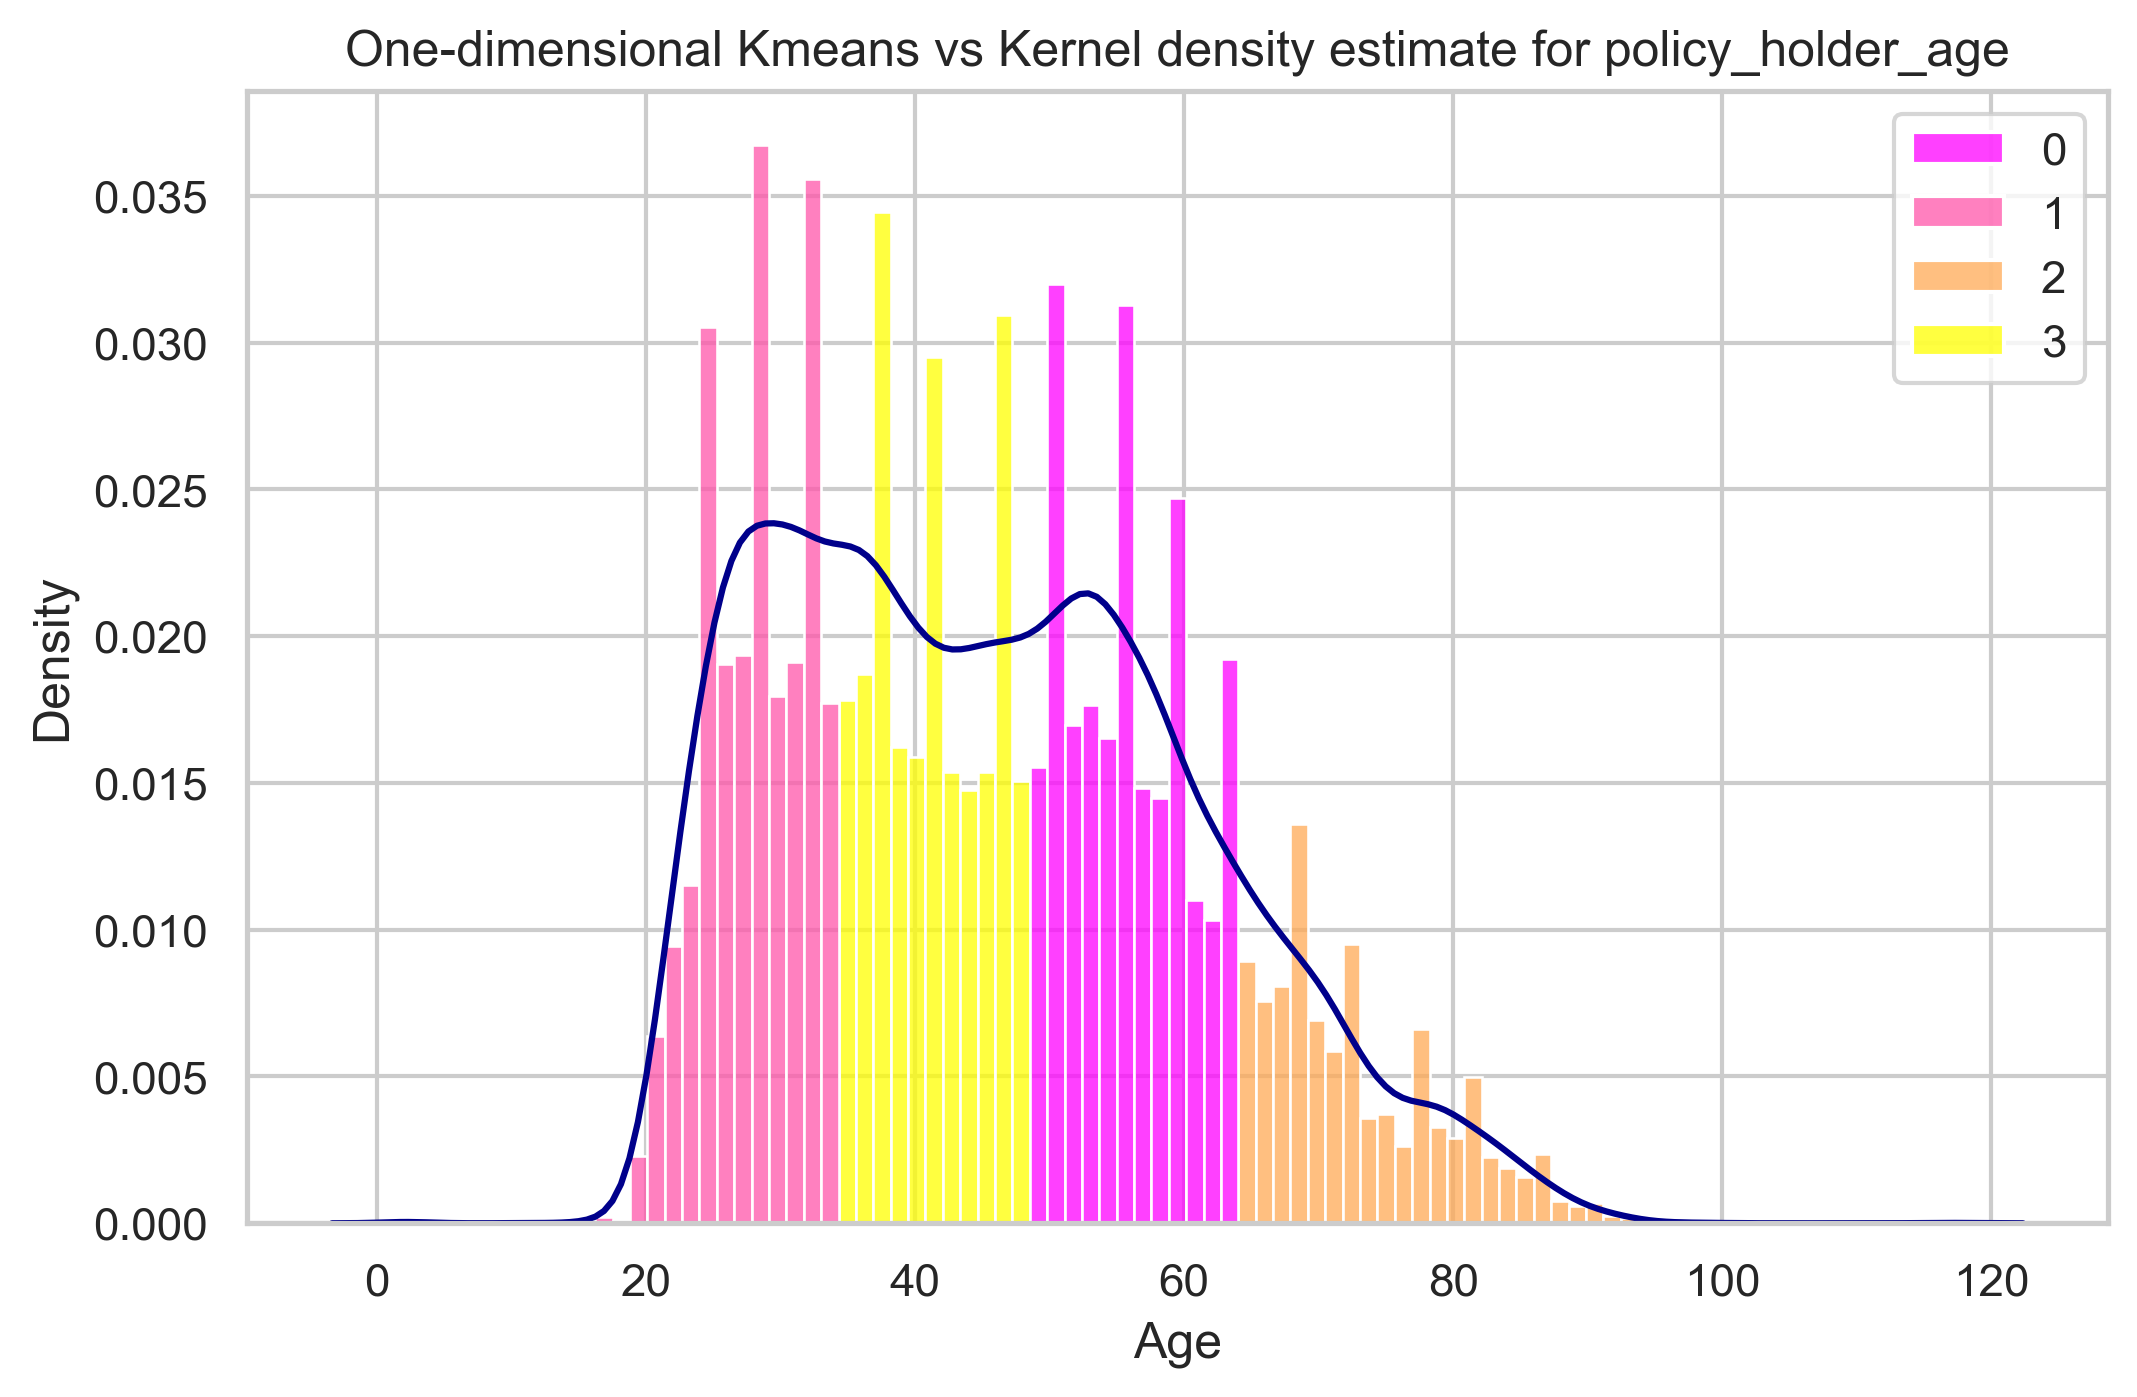
\includegraphics[width=1\linewidth]{one_dim_kmeans2}
  \label{fig:sub2}
\end{subfigure}
\vspace{-1cm}
\caption{Compare data binning results of age-related features using One-dimensional Kmeans with 4 clusters and kernel density estimates.}
\label{fig:feature_engineering_age_onedimkmeans}
\end{figure}

For time features i.e. \texttt{claim\_time\_occured}, it contains about 88.4\% of missing values and has a format of \texttt{HH:MM}. Therefore, \texttt{claim\_time\_occured} is binned in terms of hours, 00:00-01:00, 01:00-02:00,..., 23:00-24:00, and missing values are encoded as \textit{unknown}. Under this categorization, non-missing time can be kept as a feature. Other binning schemes are possible but it is natural to bin time with \texttt{HH:MM} format into hours.\\  

The dataset contains features related to the postal code, including \texttt{claim\_postal\_code}, \texttt{policy\_\\holder\_postal\_code}, \texttt{driver\_postal\_code}, \texttt{third\_party\_1\_postal\_code}, \texttt{third\_party\_2\_\\postal\_code}, \texttt{third\_party\_3\_postal\_code} and \texttt{repair\_postal\_code}. However, these features have more than 1,000 unique postal code values. Without data binning, one hot encoding will create sparse data matrix and greatly increase the dimension of dataset. To avoid a huge search space, we keep the postal codes by their information values, calculated from their weights of evidence. For imbalanced data, we considered a lower threshold for information value, and the postal codes are preserved when their information values are greater than 0.01. Otherwise, they will be grouped under the same level, namely, \textit{other} because they do not contribute much to detect fraudulent cases. A small threshold of 0.01 is used because there are many factor levels.  The results are summarized in exploratory data analysis section. For \texttt{third\_party\_3\_postal\_code}, no non-missing fraudulent cases are found, and hence we simply encode it as a dummy variable with levels \textit{known} and \textit{unknown}.

\begin{table}[h]
	\centering
	\begin{tabular}{|l|c|}
	\hline
	Postal code-related features & Number of distinct values \\
	\hline
	\texttt{claim\_postal\_code} & 1060 \\
	\texttt{policy\_holder\_postal\_code} & 1082 \\
	\texttt{driver\_postal\_code} & 1077 \\
	\texttt{third\_party\_1\_postal\_code} & 1088 \\
	\texttt{third\_party\_2\_postal\_code} & 750 \\
	\texttt{third\_party\_3\_postal\_code} & 27 \\
	\texttt{repair\_postal\_code} & 754 \\
	\hline
	\end{tabular}
	\caption{Total number of distinct postal codes for each related feature in the dataset}
\end{table}

Apart from postal code, \texttt{policy\_coverage\_type} also have many factor levels. So, weight of evidence encoding is applied for the similar reason. For other techniques, the odds-based grouping also provides similar results whereas one-dimensional k-means is only applicable to continuous features. Grouping postal code by frequency seems a less plausible method for imbalanced dataset because the grouping may be biased to the majority class. Hence, weight of evidence encoding is a good method in our case. \\

There are some id-related features in the dataset, for instance, \texttt{claim\_vehicle\_id}, \texttt{policy\_hold\\er\_expert\_id}, \texttt{third\_party\_1\_id}, \texttt{third\_party\_1\_vehicle\_id} and \texttt{third\_party\_1\_expert\_id}. As every id-related feature is anonymized, one hot encoding may also lead to a huge increase in dimension. Dummy encoding of id-related features, with known id labelled as 1 and missing id labelled as 0, gives meaningful interpretation to them.

\clearpage

\subsection*{Exploratory data analysis}
\addcontentsline{toc}{subsection}{Exploratory data analysis}

In the exploratory analysis, most graphs are visualized using \texttt{seaborn} and \texttt{matplotlib} in python. Treemaps are visualized using \texttt{squarify}.

\subsubsection*{Class imbalance problem}
\addcontentsline{toc}{subsubsection}{Class imbalance problem}

Class imbalance problem makes the classification task harder. In the dataset, 55,155 cases are non-fraudulent, and 308 cases are fraudulent which accounts for 0.56\% of the total sample, as summarized in figure 6. There are very few fraudulent cases in the dataset, and hence the dataset is imbalanced. It suggests some sampling techniques e.g. oversampling or smart sampling as well as metrics (other than accuracy) are needed in the training process so as to overcome the class imbalance problem.

\begin{figure}[h]
\centering
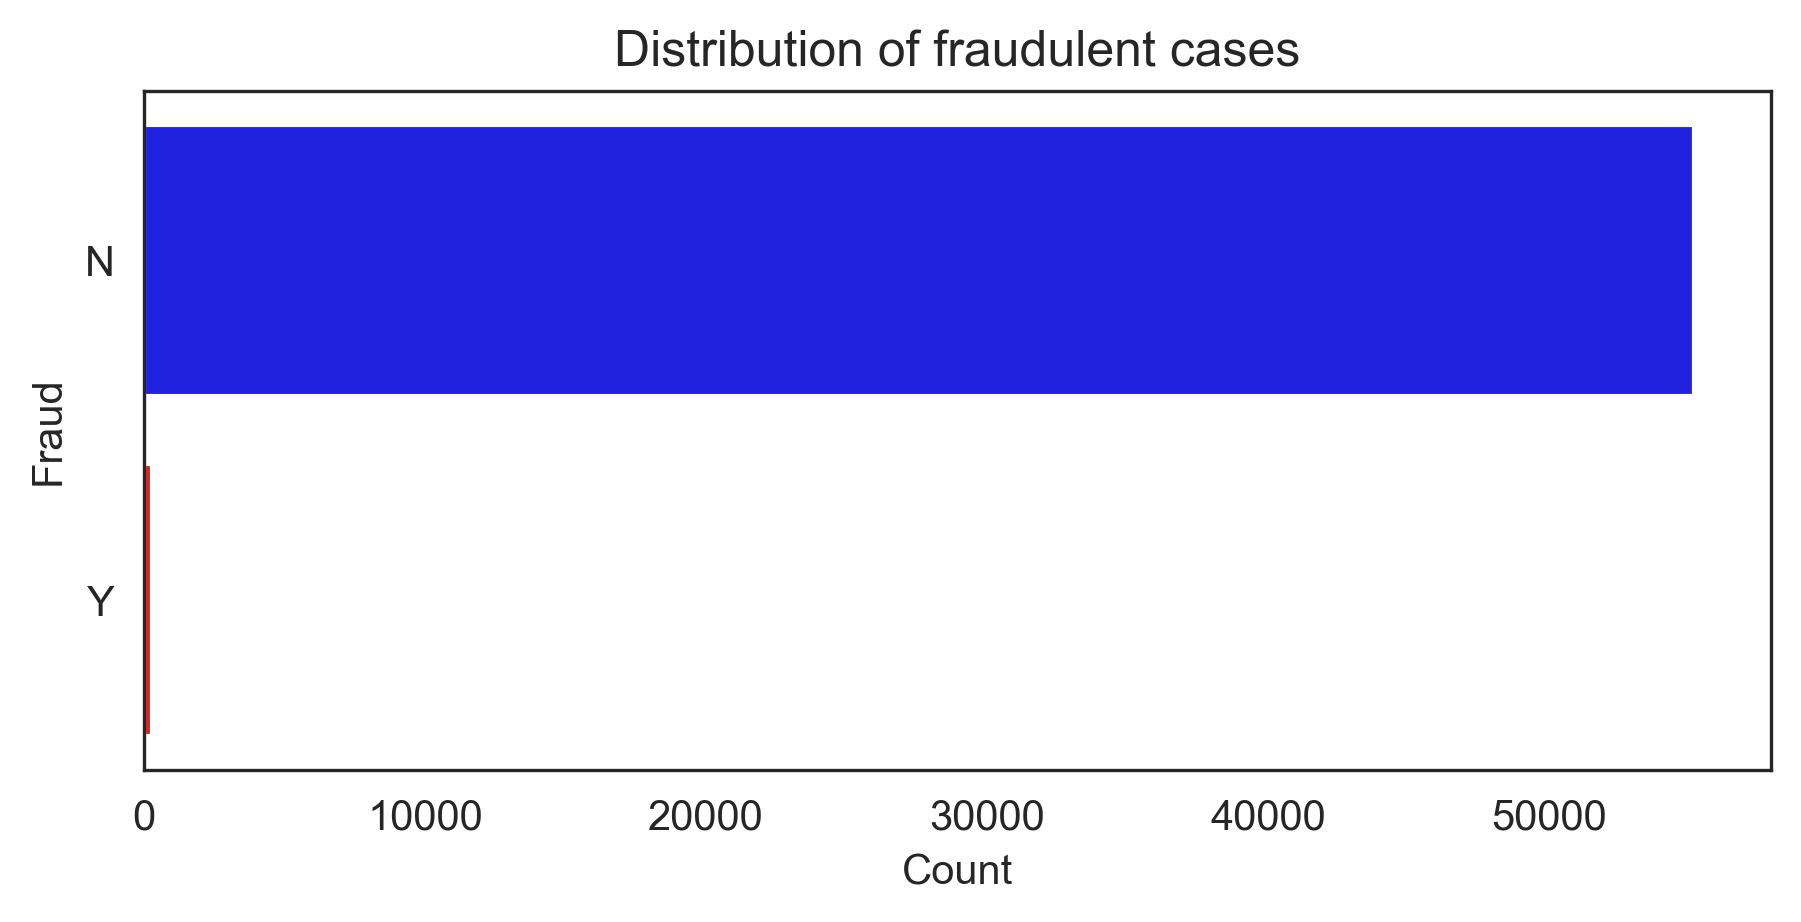
\includegraphics[width = 12cm]{class_imbal_problem}
\vspace{-0.5cm}
\caption{Barplot for \texttt{fraud}}
\end{figure}

\vspace{-1cm}
\subsubsection*{Descriptive statistics}
\addcontentsline{toc}{subsubsection}{Descriptive statistics}

To develop a basic understanding of the training data, some features are covered in this section. The feature \texttt{claim\_amount} is only provided in the training data which serves as a weighting variable in scoring because the goal of the classification task is to predict the probabilities of top 100 fraudulent cases in terms of their insurance claim amounts. In figure 7, we observe the distribution for \texttt{claim\_amount} is highly right-skewed. Some observations have very high claiming amounts. In general, fraudulent cases tend to have higher claim amounts as their median and the upper quartile are much higher than those of non-fraudulent cases. Still, there are some non-fraudulent cases having high claim amounts. 

\begin{figure}[h]
\centering
\begin{subfigure}{.5\textwidth}
  \centering
  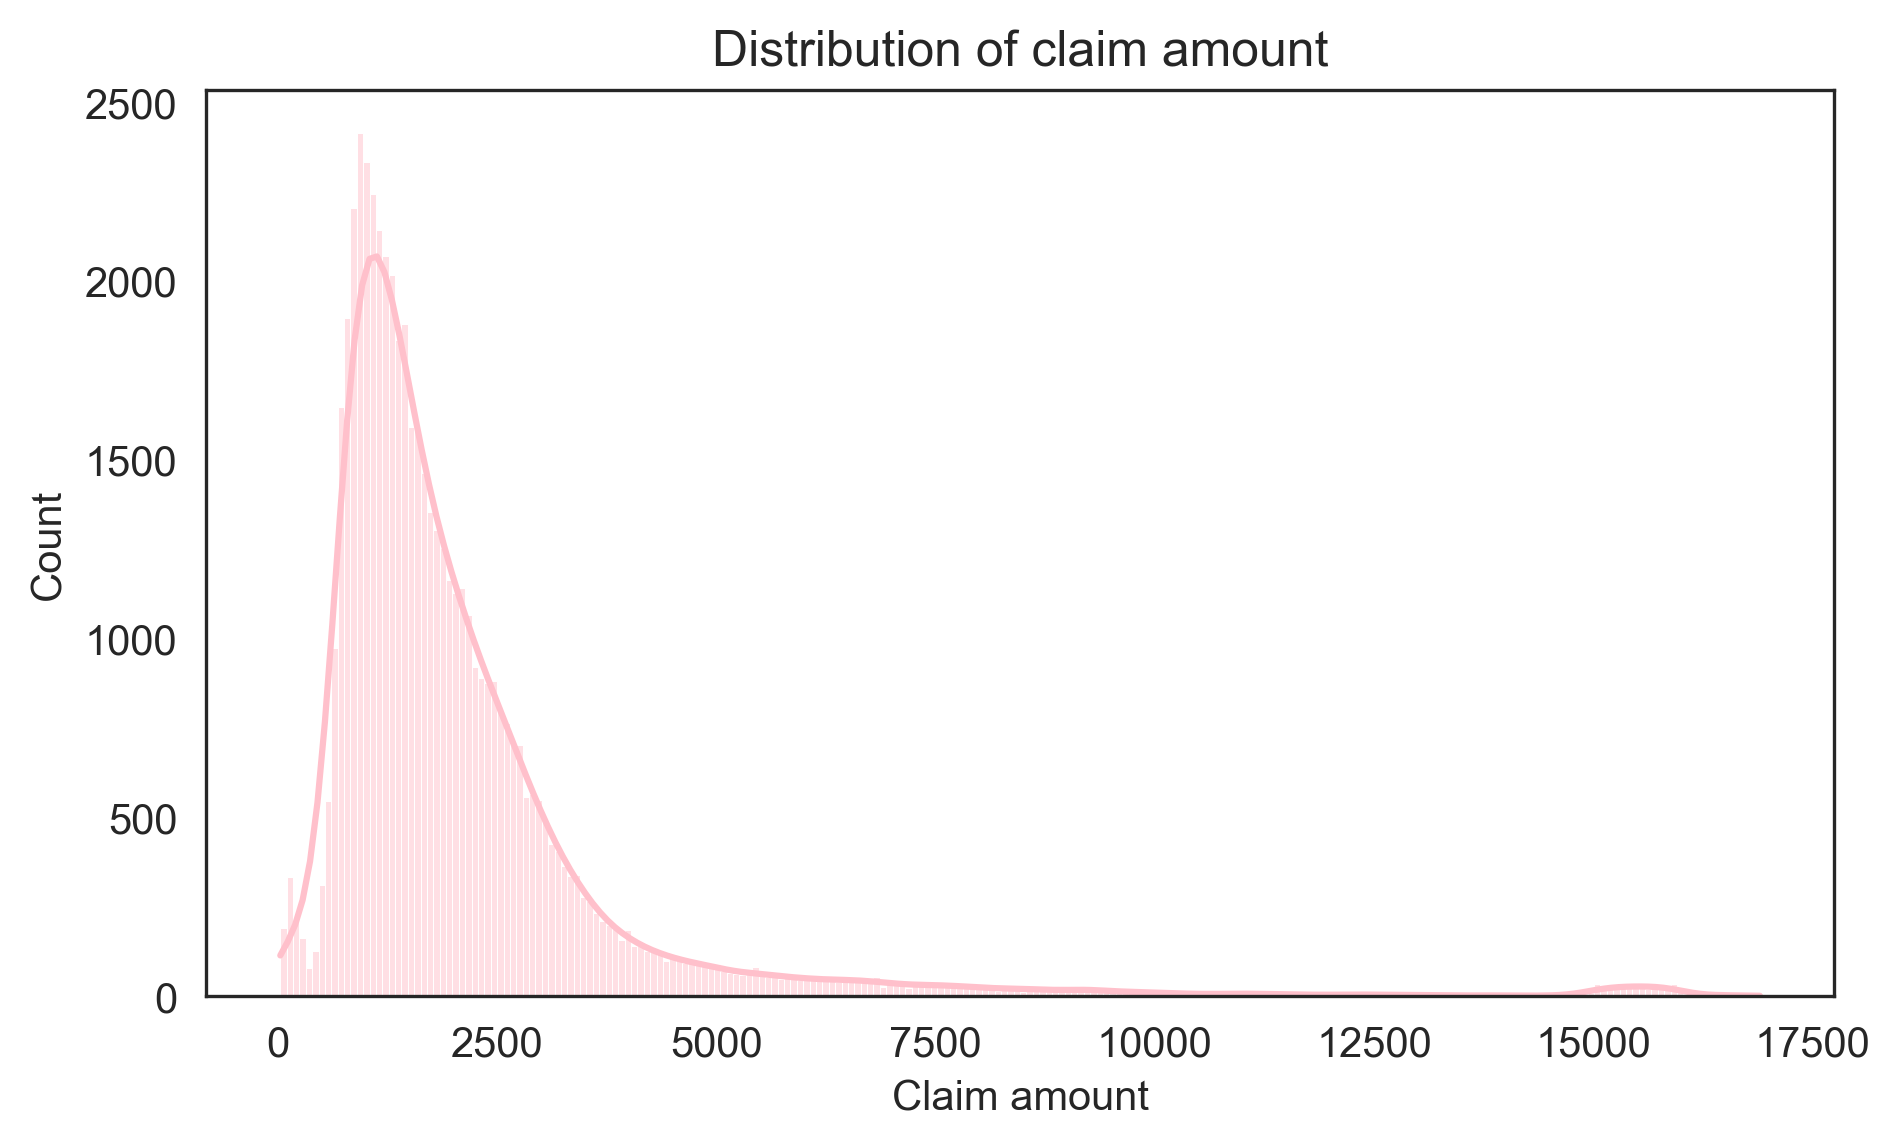
\includegraphics[width=1\linewidth]{dist_claim_amount}
  \label{fig:sub1}
\end{subfigure}%
\begin{subfigure}{.5\textwidth}
  \centering
  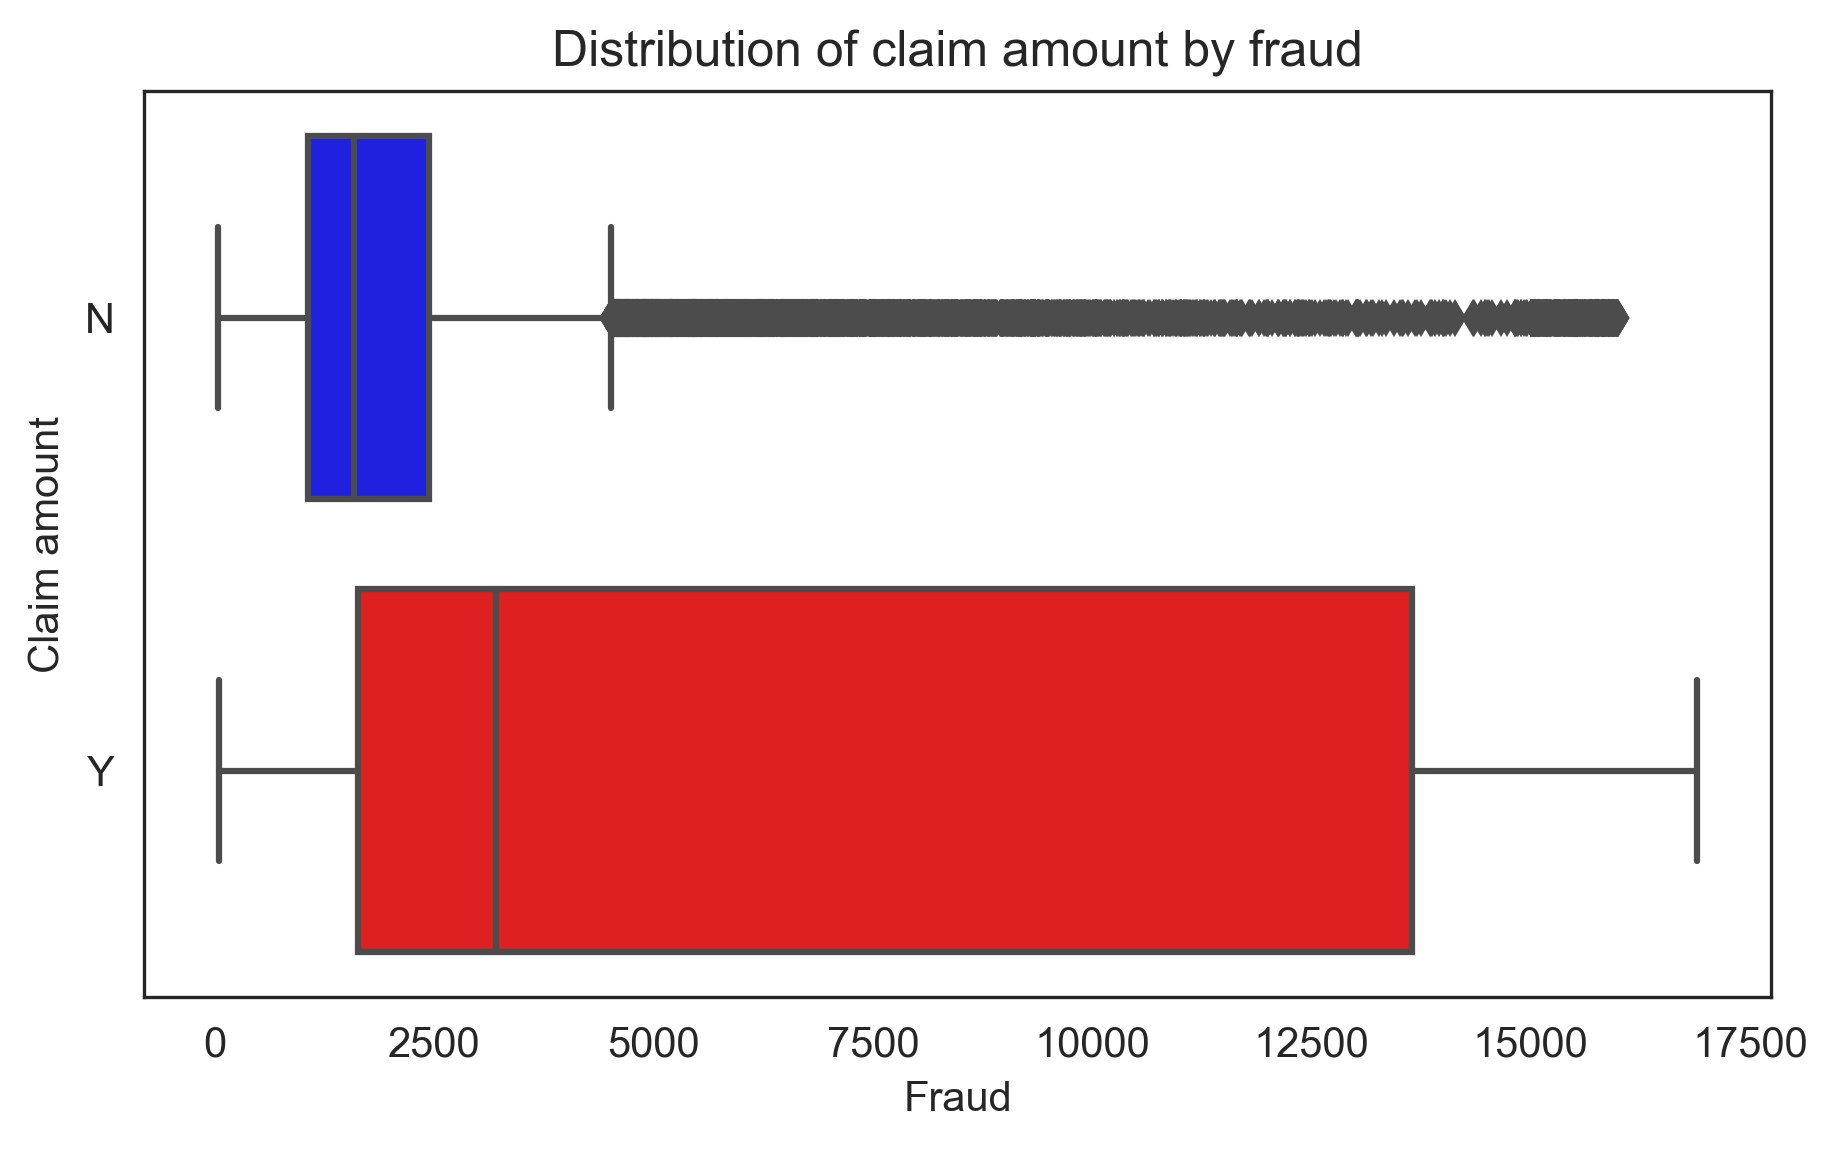
\includegraphics[width=1\linewidth]{dist_claim_amount_by_fraud}
  \label{fig:sub2}
\end{subfigure}
\vspace{-1cm}
\caption{Distribution of \texttt{claim\_amount}}
\label{fig:test}
\end{figure}

A brief summary of categorical features is presented in figure 8 as barplots. For continuous features, their boxplots are presented in figure 9.

\begin{figure}[h]
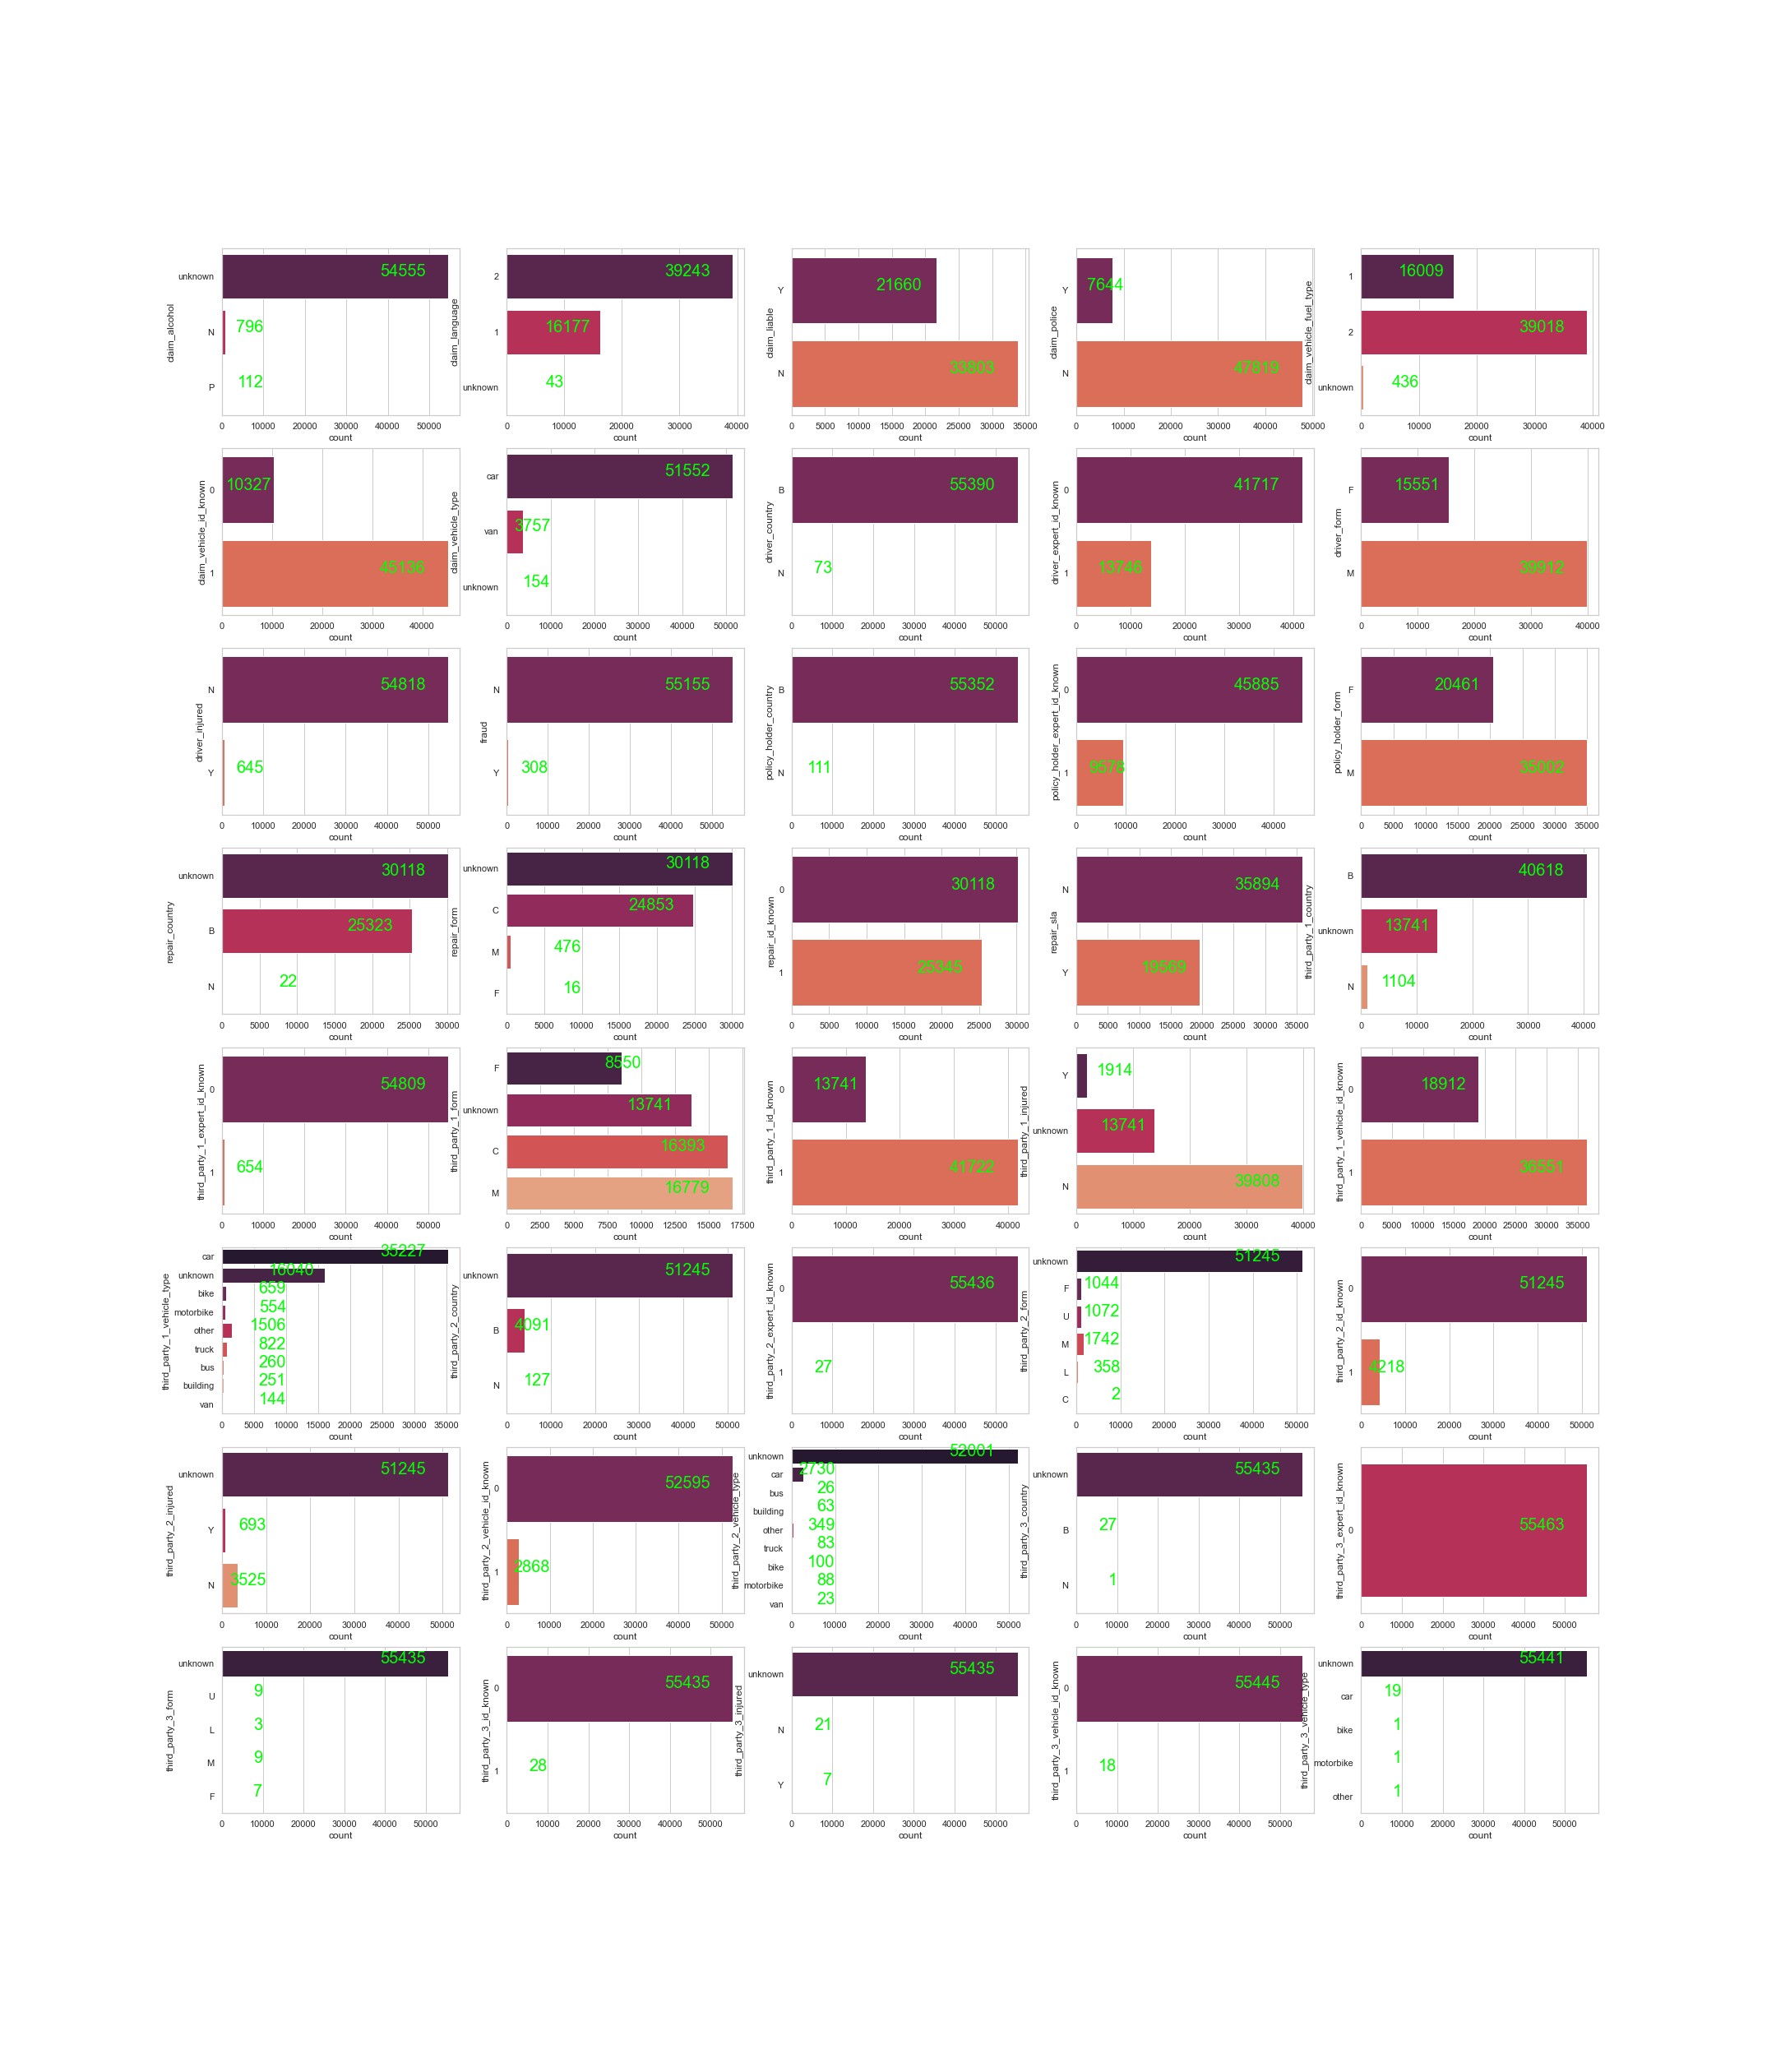
\includegraphics[width = 20cm, height = 25cm,
trim = {11cm 5cm 0 5cm}]{binary_barplot}
\vspace{-2cm}
\caption{Summary of categorical features. Features with too many factor levels e.g. postal-code or vehicle brands are not included in this plot}
\end{figure}

\begin{figure}[h]
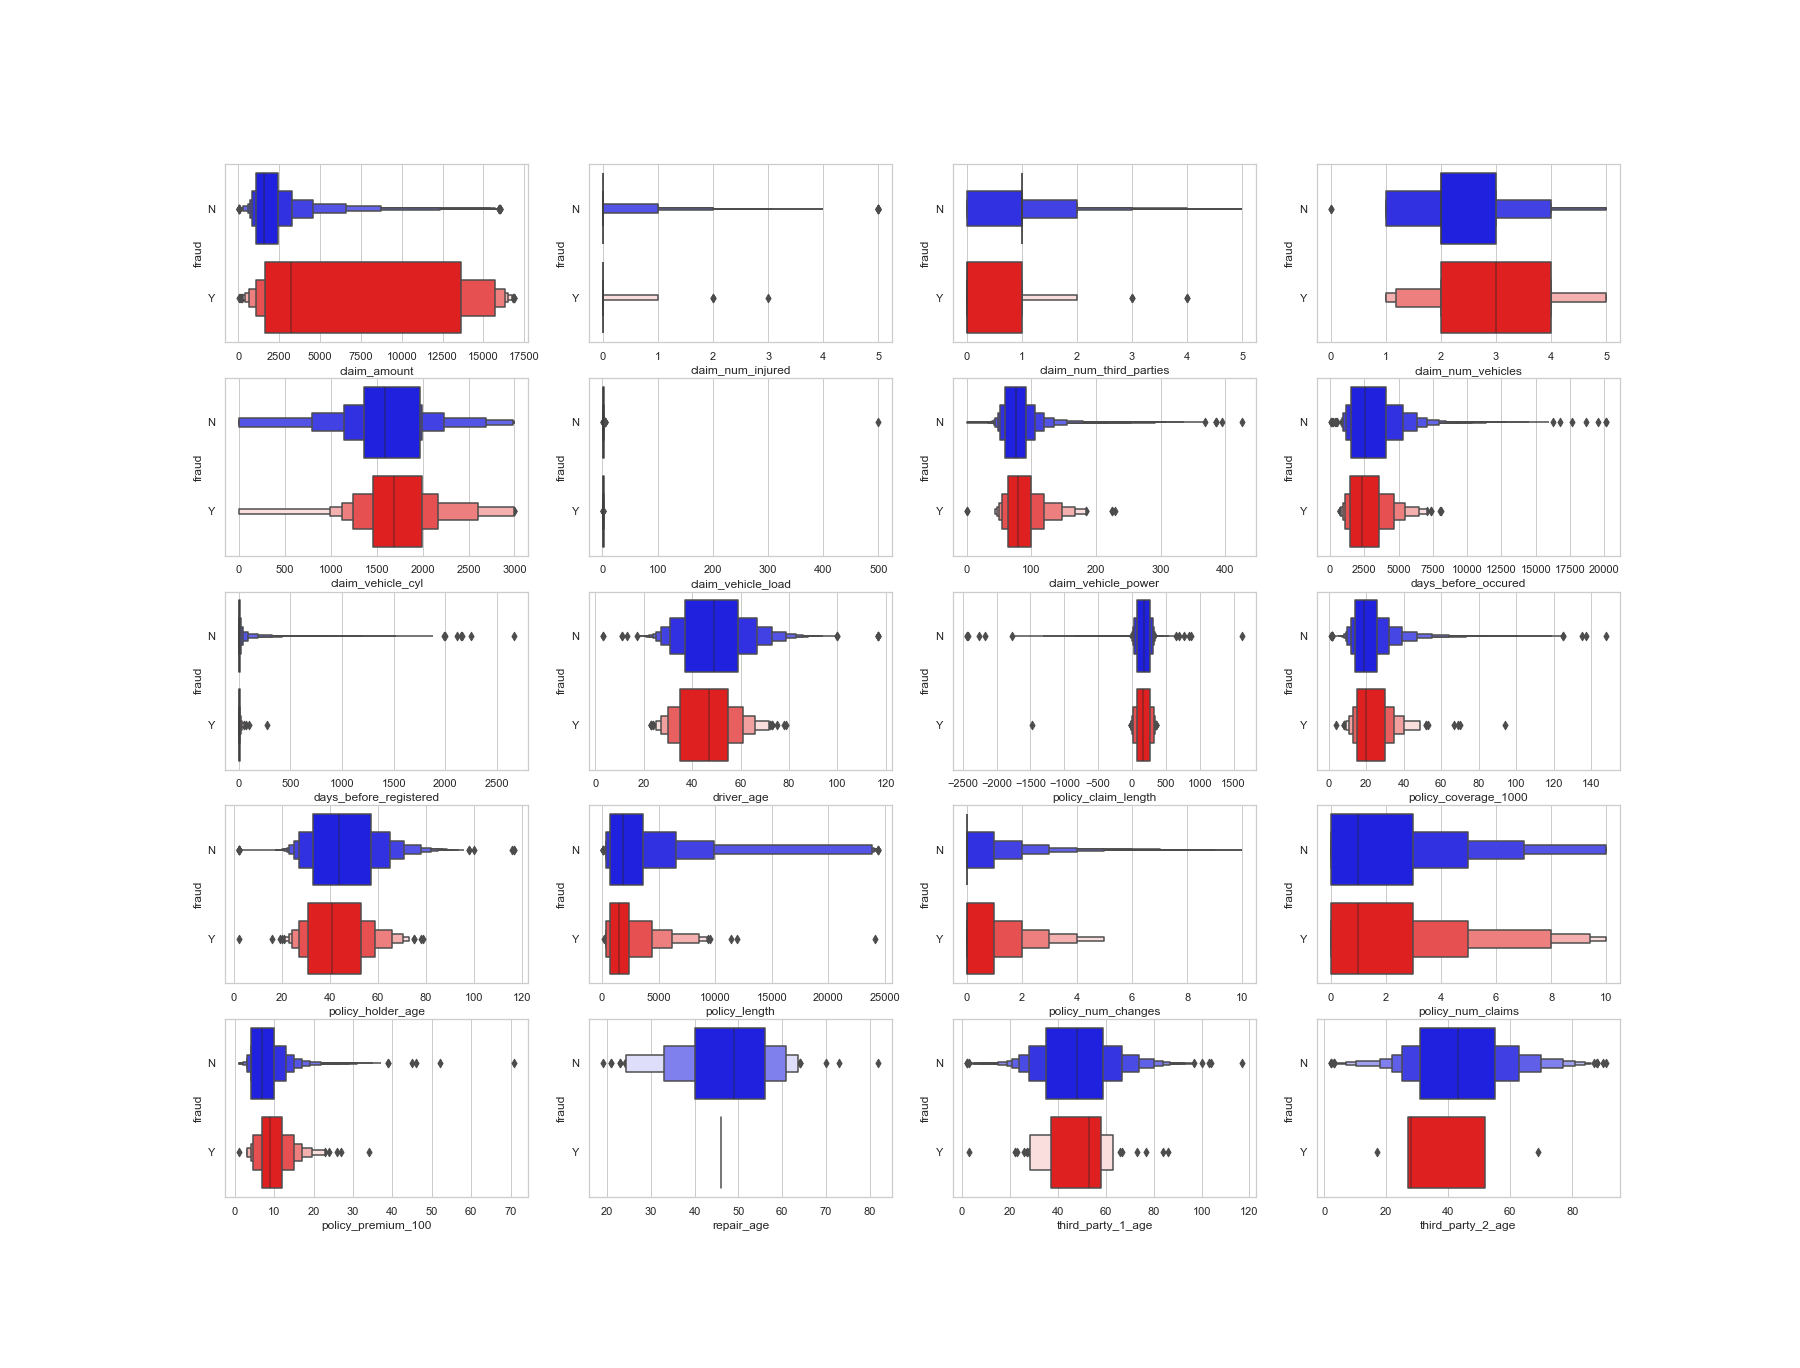
\includegraphics[width = 20cm, height = 23cm,
trim = {8cm 0cm 0 0cm}]{cont_boxplot}
\vspace{-2cm}
\caption{Summary of continuous features grouped by fraudulent status}
\end{figure}

\clearpage
The dataset contains some features related to the third parties, and \texttt{claim\_num\_third\_party} indicates the number of third parties involved. There are about 69\% of cases involved exactly one third party. About 24.7\% of cases do not involve any third party, and only 6.3\% of cases involve more than one third party. The average claim amounts and frequency of the number of third party conditioned on fraudulent status are summarized as heatmaps presented in figure 10. For fraudulent cases, about 58\% of observations do not have third party, and 39\% of them have one third party. Unlike non-fraudulent cases, about 69\% of observations have one third party and only 25\% of them have no third party. However, in terms of average claim amounts, fraudulent cases have high values for instances with more than one third party. It means features related to the second and the third third parties may be useful in classification.\\

\vspace{-0.5cm}
\begin{figure}[h]
\centering
\begin{subfigure}{.6\textwidth}
  \centering
  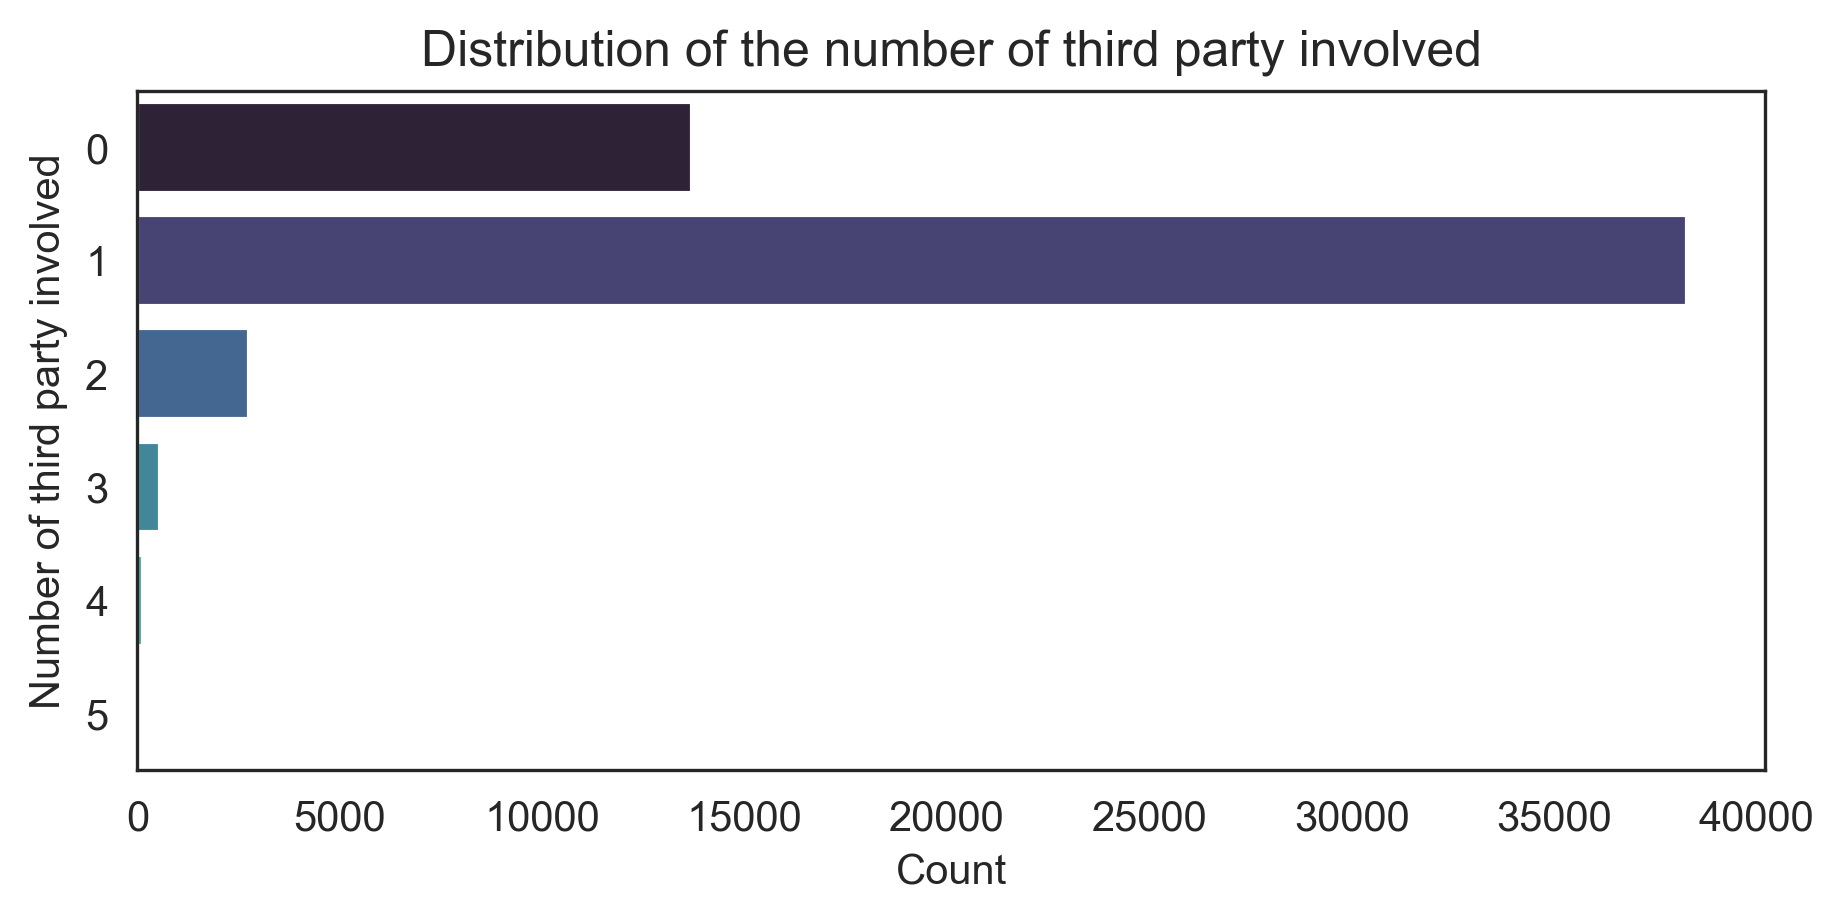
\includegraphics[width=1\linewidth]{num_third_party_involved}
  \label{fig:sub1}
\end{subfigure}%
\begin{subfigure}{.4\textwidth}
  \centering
  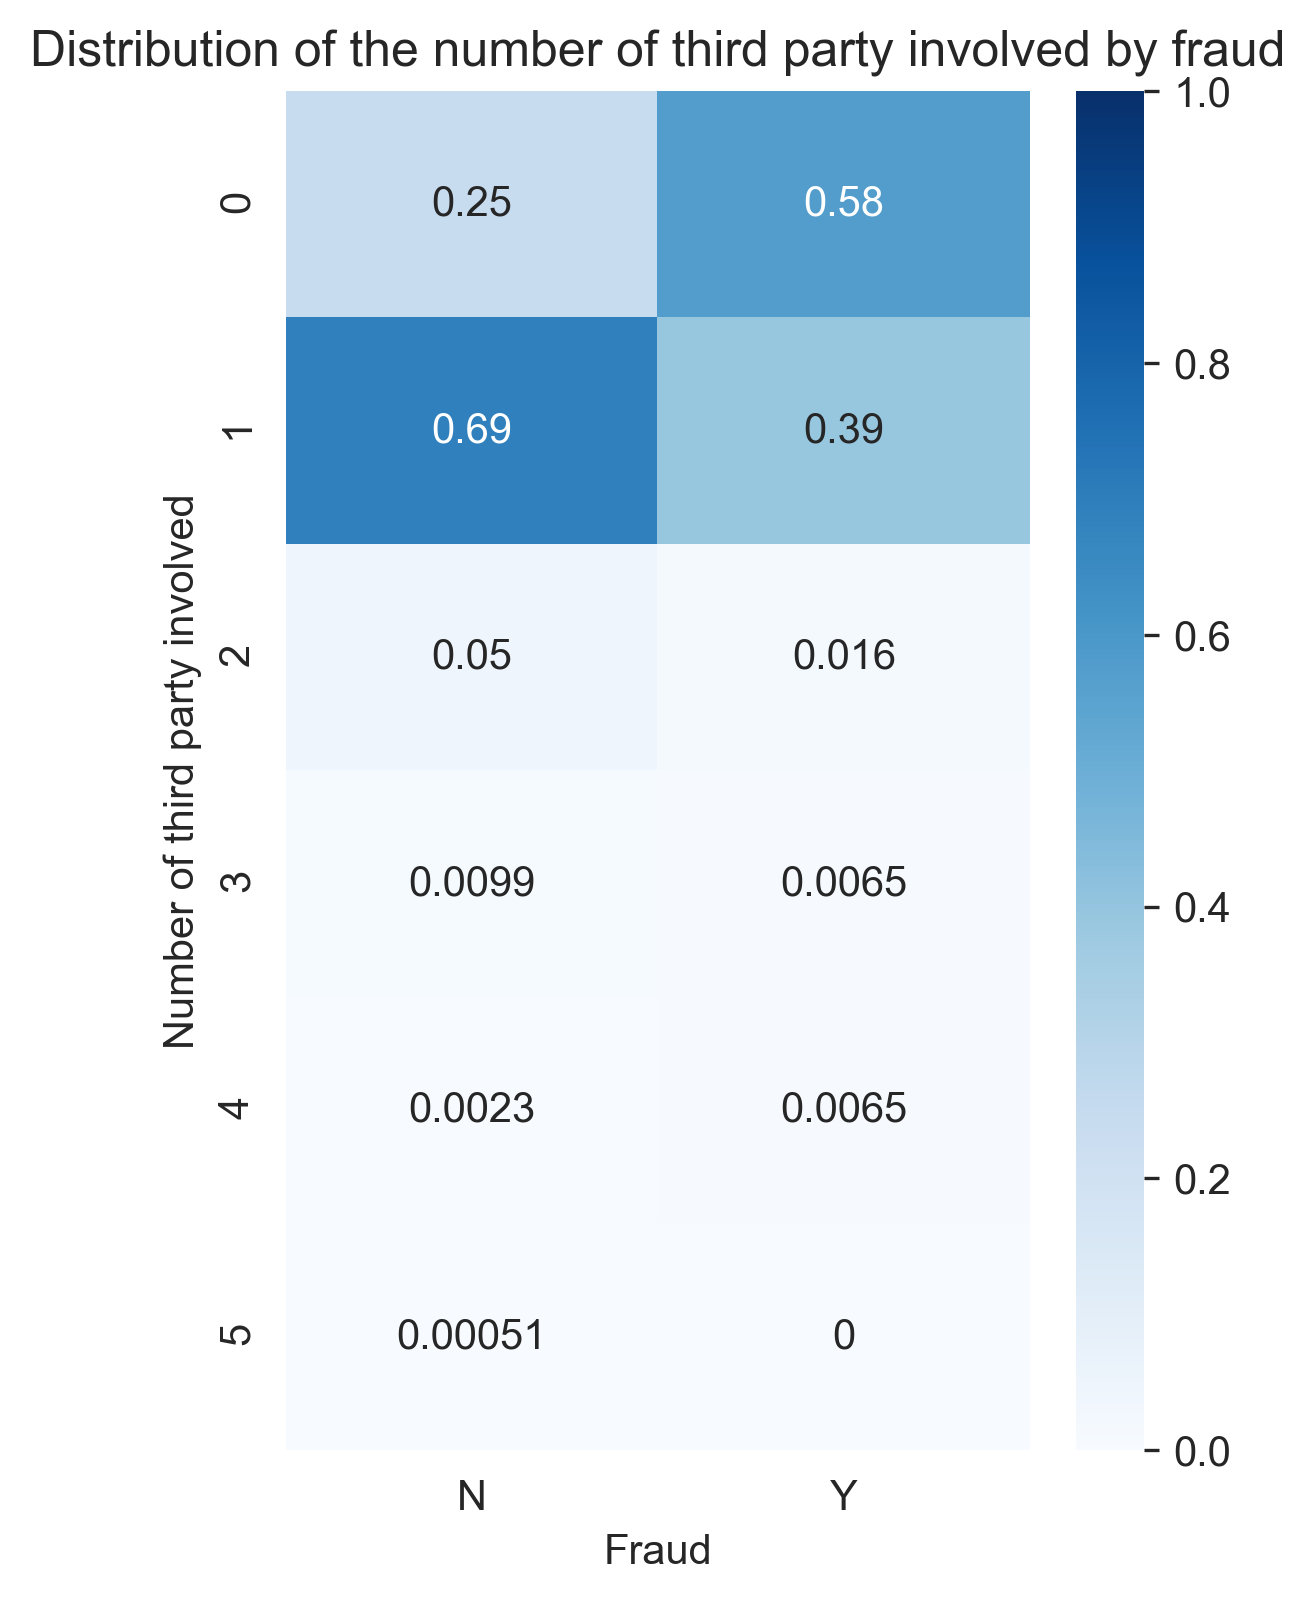
\includegraphics[width=1\linewidth]{num_third_party_involved_by_fraud}
  \label{fig:sub2}
\end{subfigure}

\begin{subfigure}{0.7\textwidth}
  \centering
  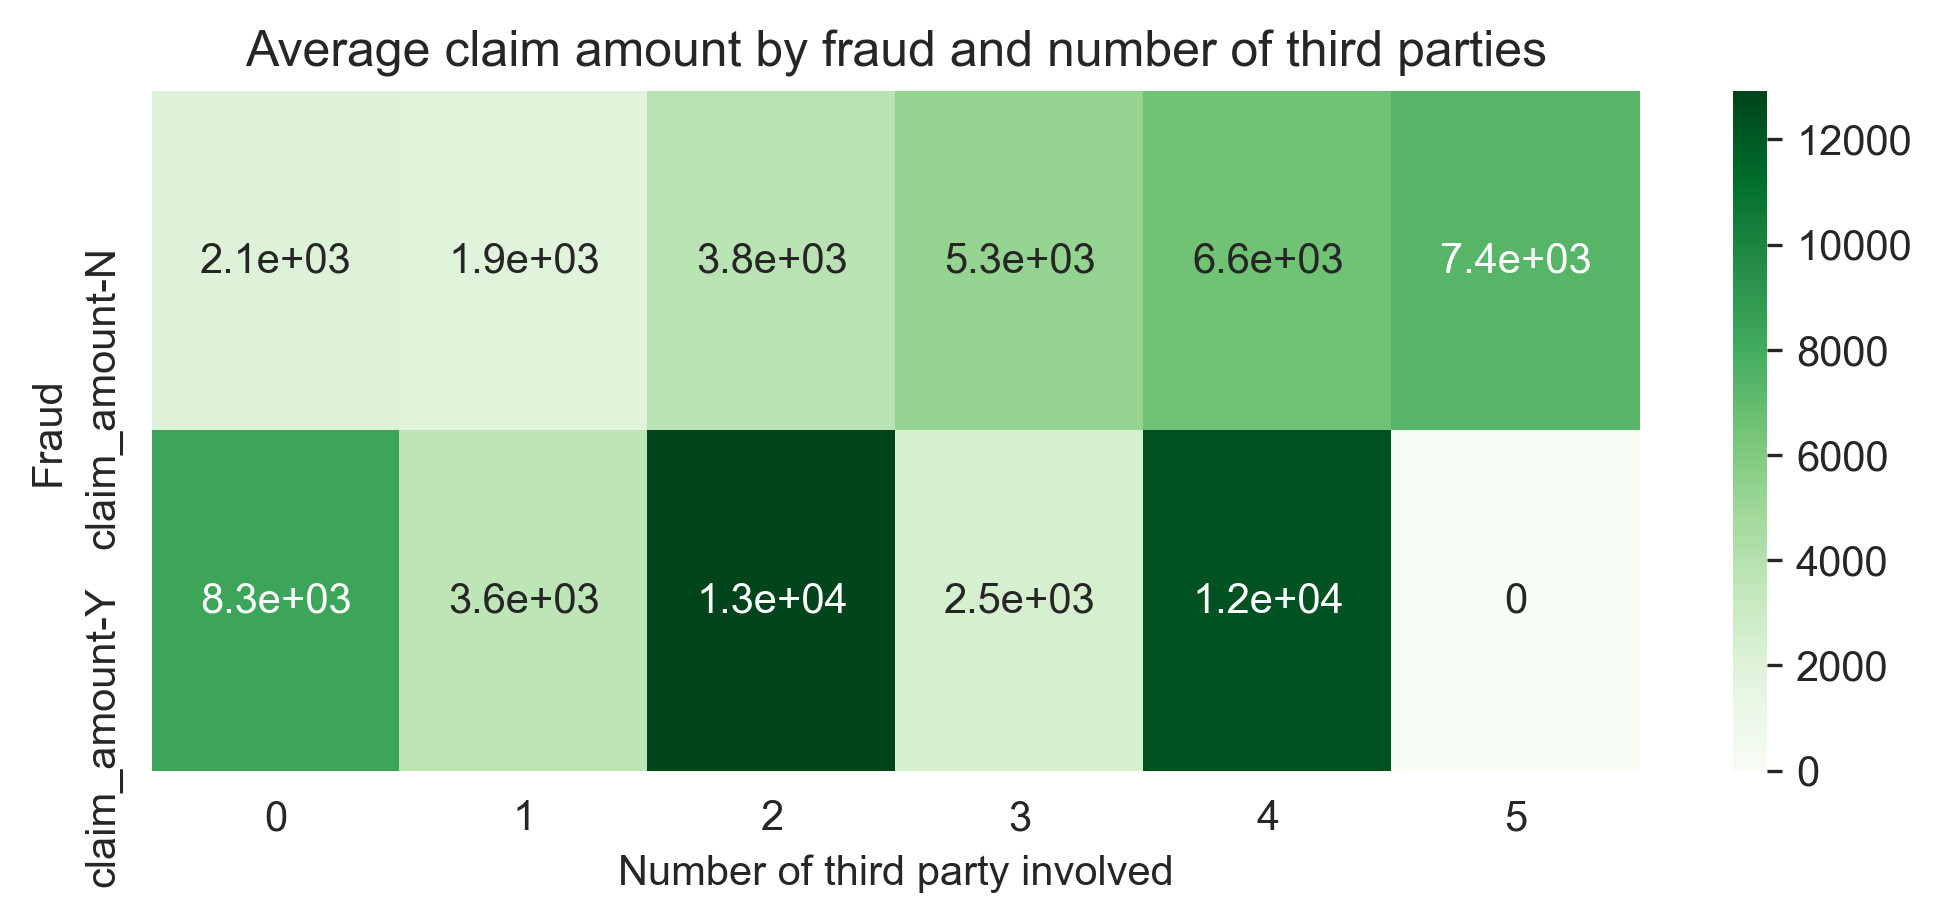
\includegraphics[width=1\linewidth]{num_third_party_involved_by_fraud2}
  \label{fig:sub2} 
\end{subfigure}
\caption{Distributions of \texttt{claim\_num\_third\_parties} with barplot and heatmaps}
\label{fig:eda_third_party_num}
\end{figure}

To know whether the occurrence of fraudulent cases and their claim amounts vary across vehicle brands, we visualize \texttt{claim\_vehicle\_brand} using treemaps from \texttt{squarify} library in python. In figure 11, it is clear that vehicles from Porsche, Land Rover and Toyota have the highest average claiming amounts for fraudulent cases. The average claiming amounts are \$15,861 for Porsche, \$15,328 for Land Rover and \$11,640 for Toyota. However, most of the fraudulent cases do not have vehicle brands recorded, which are labelled as \textit{unknown} in figure 12. Apart from missing cases, BMW, Volkswagen and Citroen are found to be most frequent fraudulent cases. \\

\begin{figure}[h]
\centering
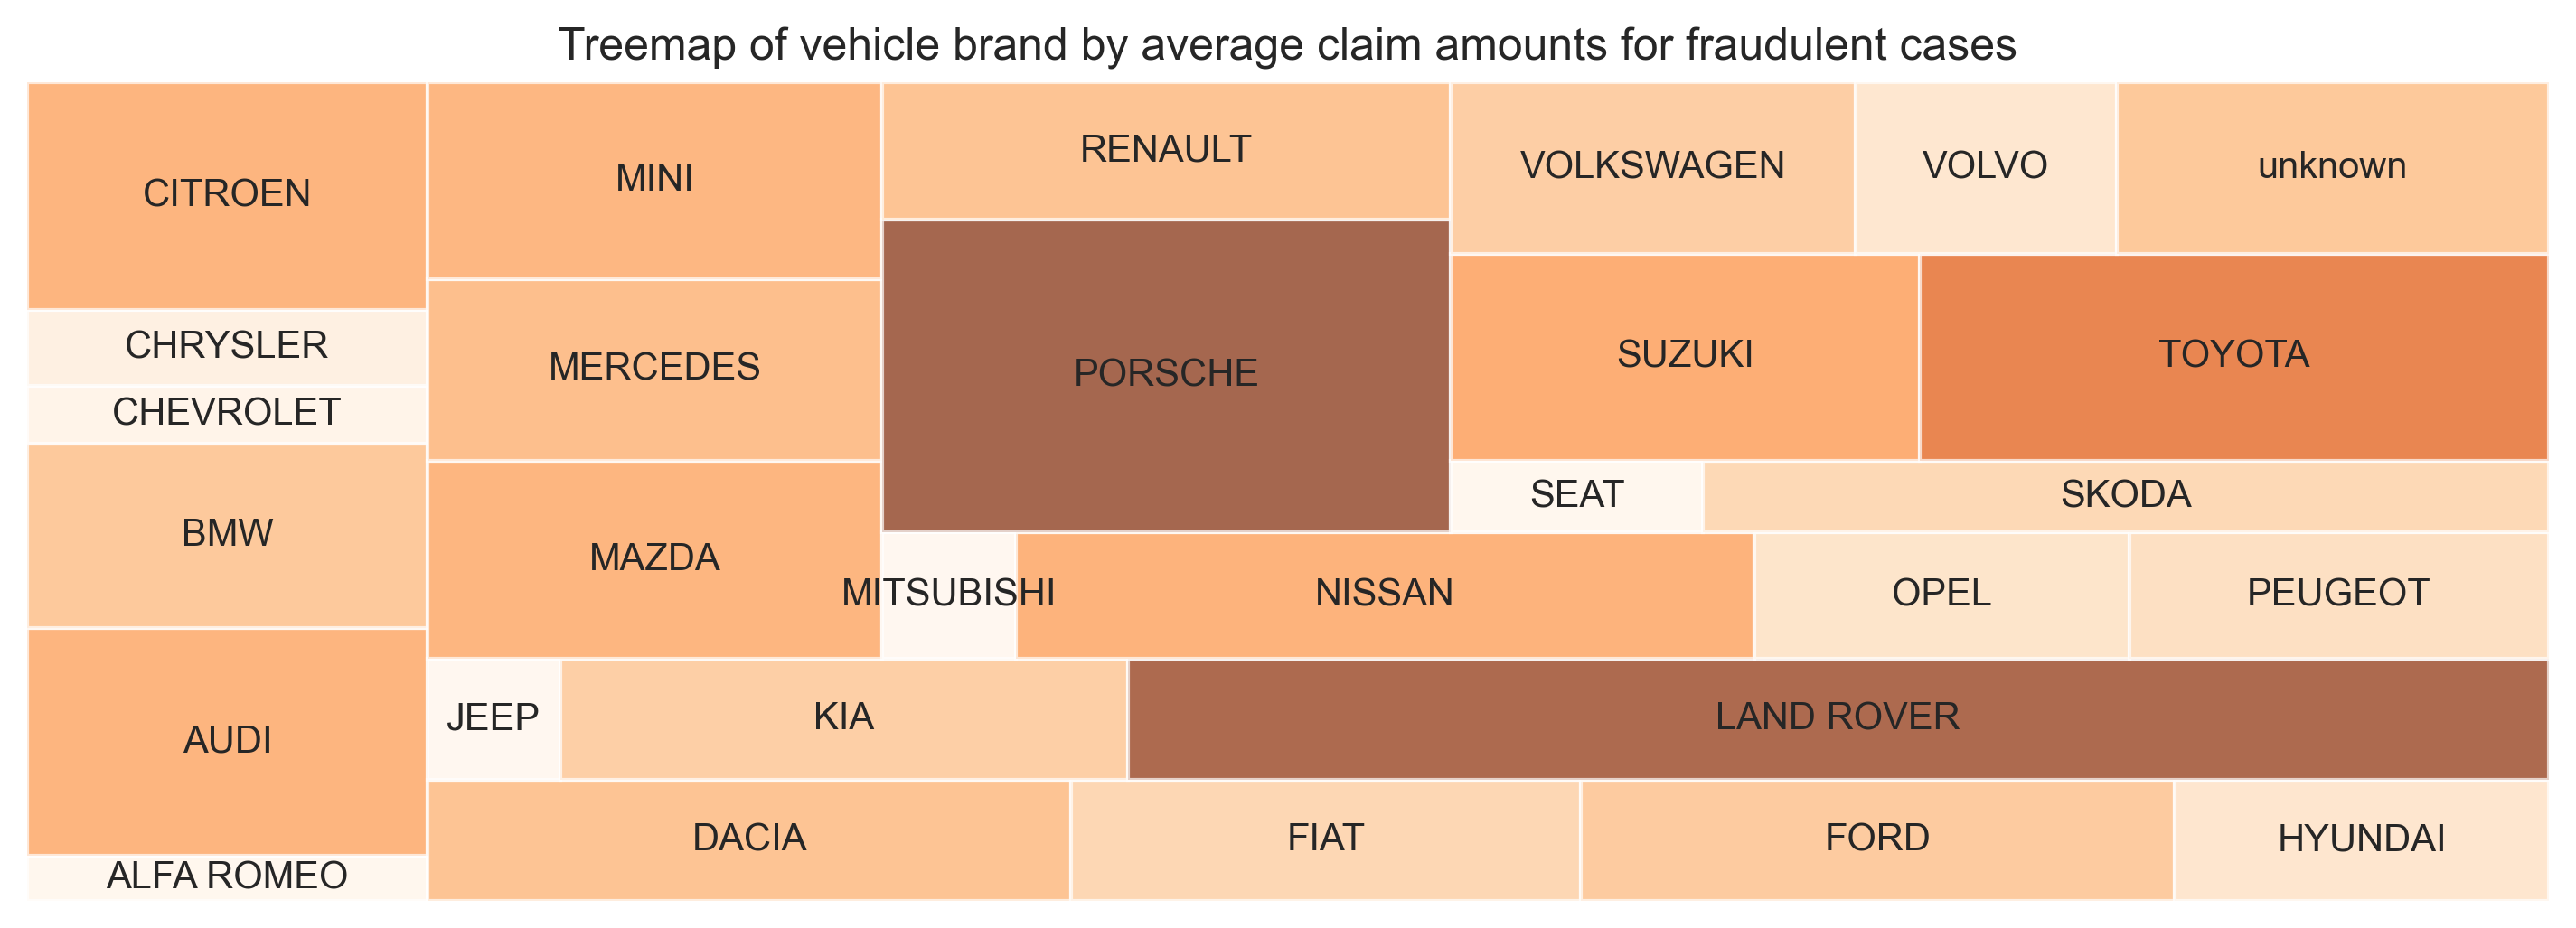
\includegraphics[width = 13cm, height = 6cm]{treemap_vehicle_brand_average_claim_amount}
\caption{Average claim amounts of fraudulent cases for different vehicle brands}
\vspace{0.5cm}
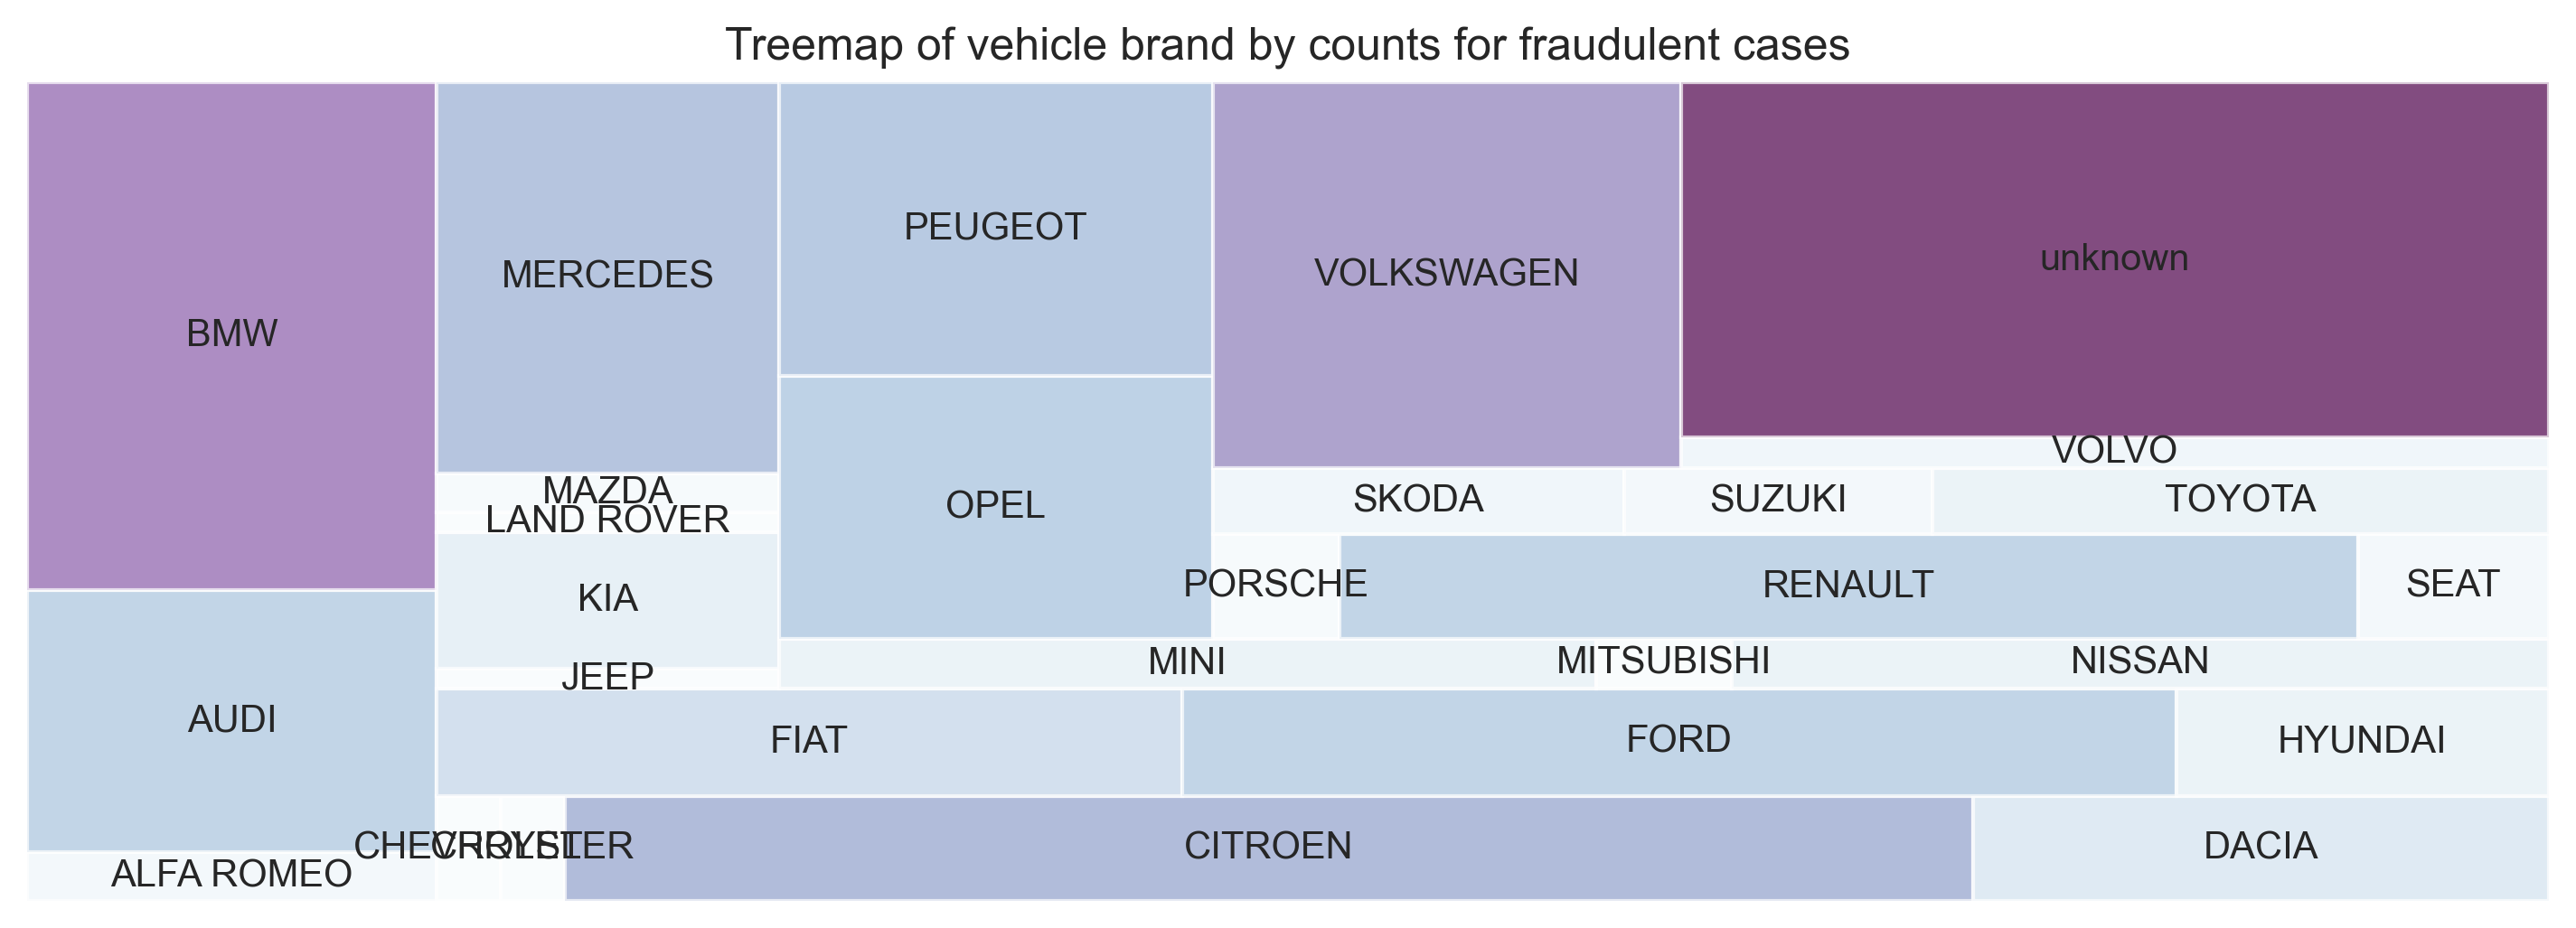
\includegraphics[width = 13cm, height = 6cm]{treemap_vehicle_brand_count}
\caption{Counts of fraudulent cases for different vehicle brands}
\vspace{0.5cm}
\end{figure}

Among various claim causes, we found that \textit{fire} and \textit{theft} are associated with higher claim amounts. The most frequent causes for fraudulent cases are \textit{traffic accident}, \textit{theft} and \textit{other}. In the training data, there are only few observations for \textit{windows}, \textit{weather} and \textit{vandalism}. The violinplot in figure 13 summarizes the findings. 

\begin{table}[h]
	\begin{tabular}{|c|cccccccc|}
	\hline
	\texttt{claim\_cause} & animal & fire & other & theft & traffic accident & vandalism & weather & windows \\
	\hline
	\texttt{fraud} = N & 334 & 29 & 7379 & 513 & 43366 & 198 & 744 & 2592 \\
	\texttt{fraud} = Y & 10 & 10 & 56 & 97 & 130 & 0 & 4 & 1\\
	\hline
	\end{tabular}
	\caption{Counts by \texttt{fraud} and \texttt{claim\_cause}}
\end{table}


As discussed in previous section, \texttt{claim\_time\_occured} is binned into 24 hours. Therefore, we can analyze the frequency of claim causes in 24 hours in an exploratory way. A heatmap on the frequency of claim causes across time for non-missing data is presented in figure 14. We observe that the claims due to \textit{animal} usually occur at 06:00 - 07:00 and 22:00 - 23:00. The claims due to \textit{fire} occur most frequently at the afternoon (from 16:00 to 18:00). There is no special time pattern for the claims due to \textit{other}. The claims due to \textit{theft} occur most frequently at 03:00-04:00, and the claims due to \textit{traffic accident} occur at the working time period (07:00-21:00). The claims due to \textit{vandalism} usually occur at 10:00-11:00 and 15:00-16:00. The claims due to \textit{weather} usually occur at 16:00-18:00, and the claims due to \textit{windows} usually occur at 12:00-13:00.

\begin{figure}[h]
\centering
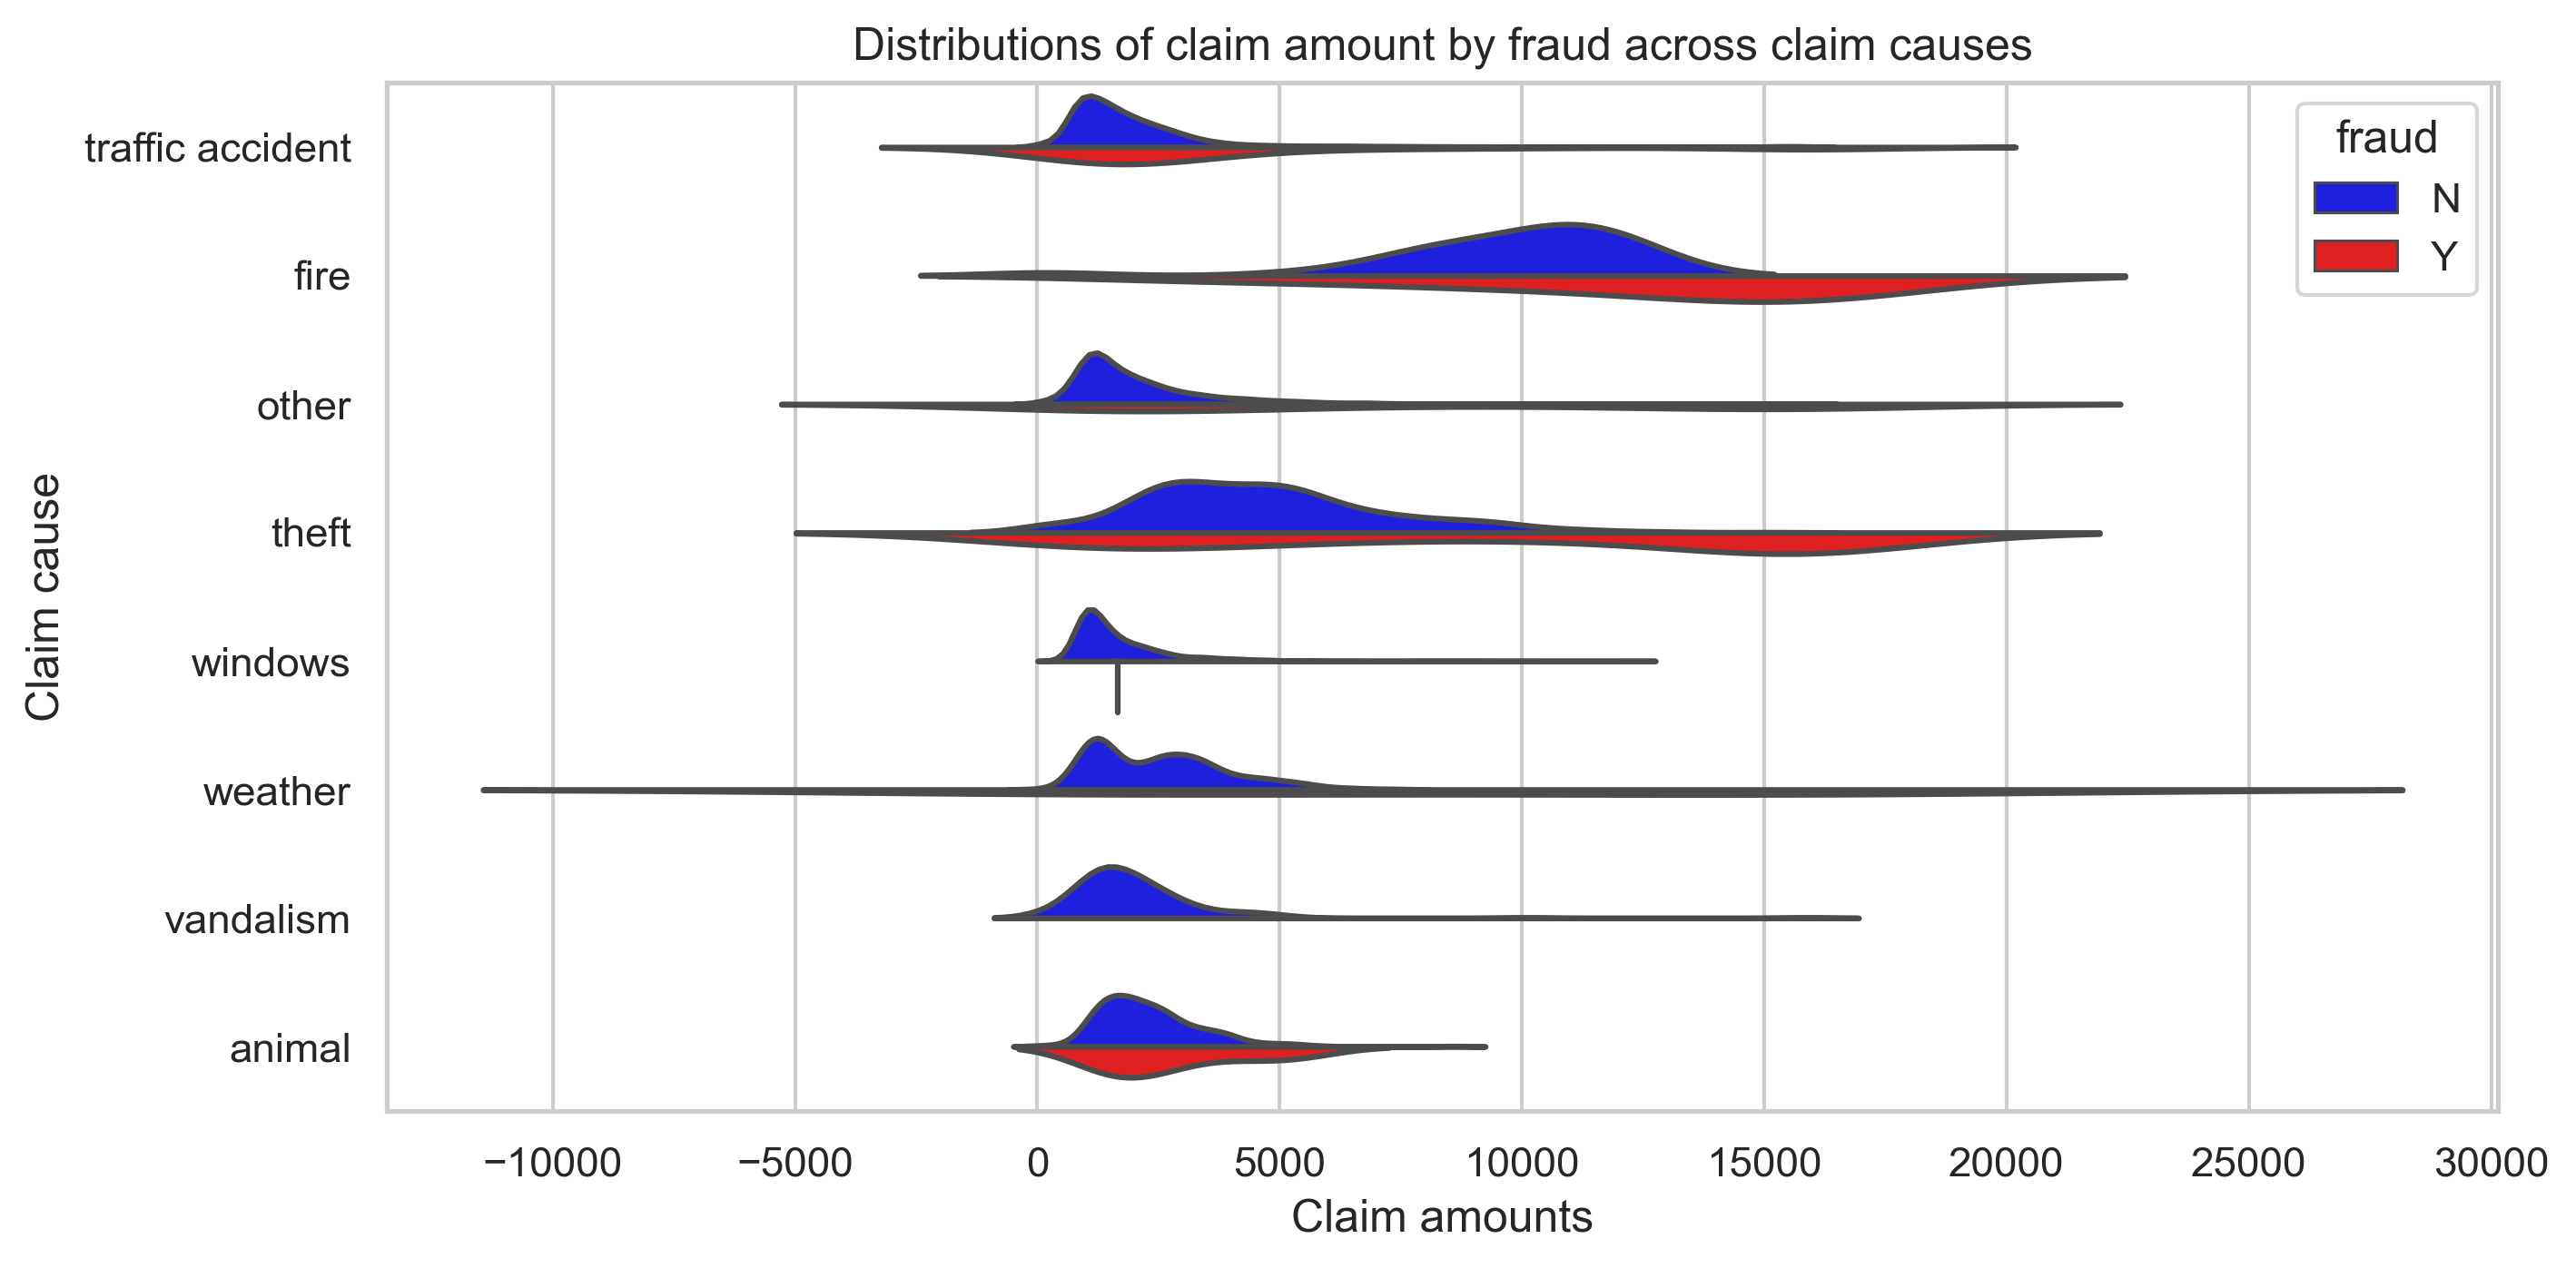
\includegraphics[width = 14cm, height = 8.5cm]{violin_plt_claim_amt_by_fraud_across_causes}
\caption{Distributions of claim amounts by fraudulent status and claim causes}
\end{figure}

\begin{figure}[h]
\centering
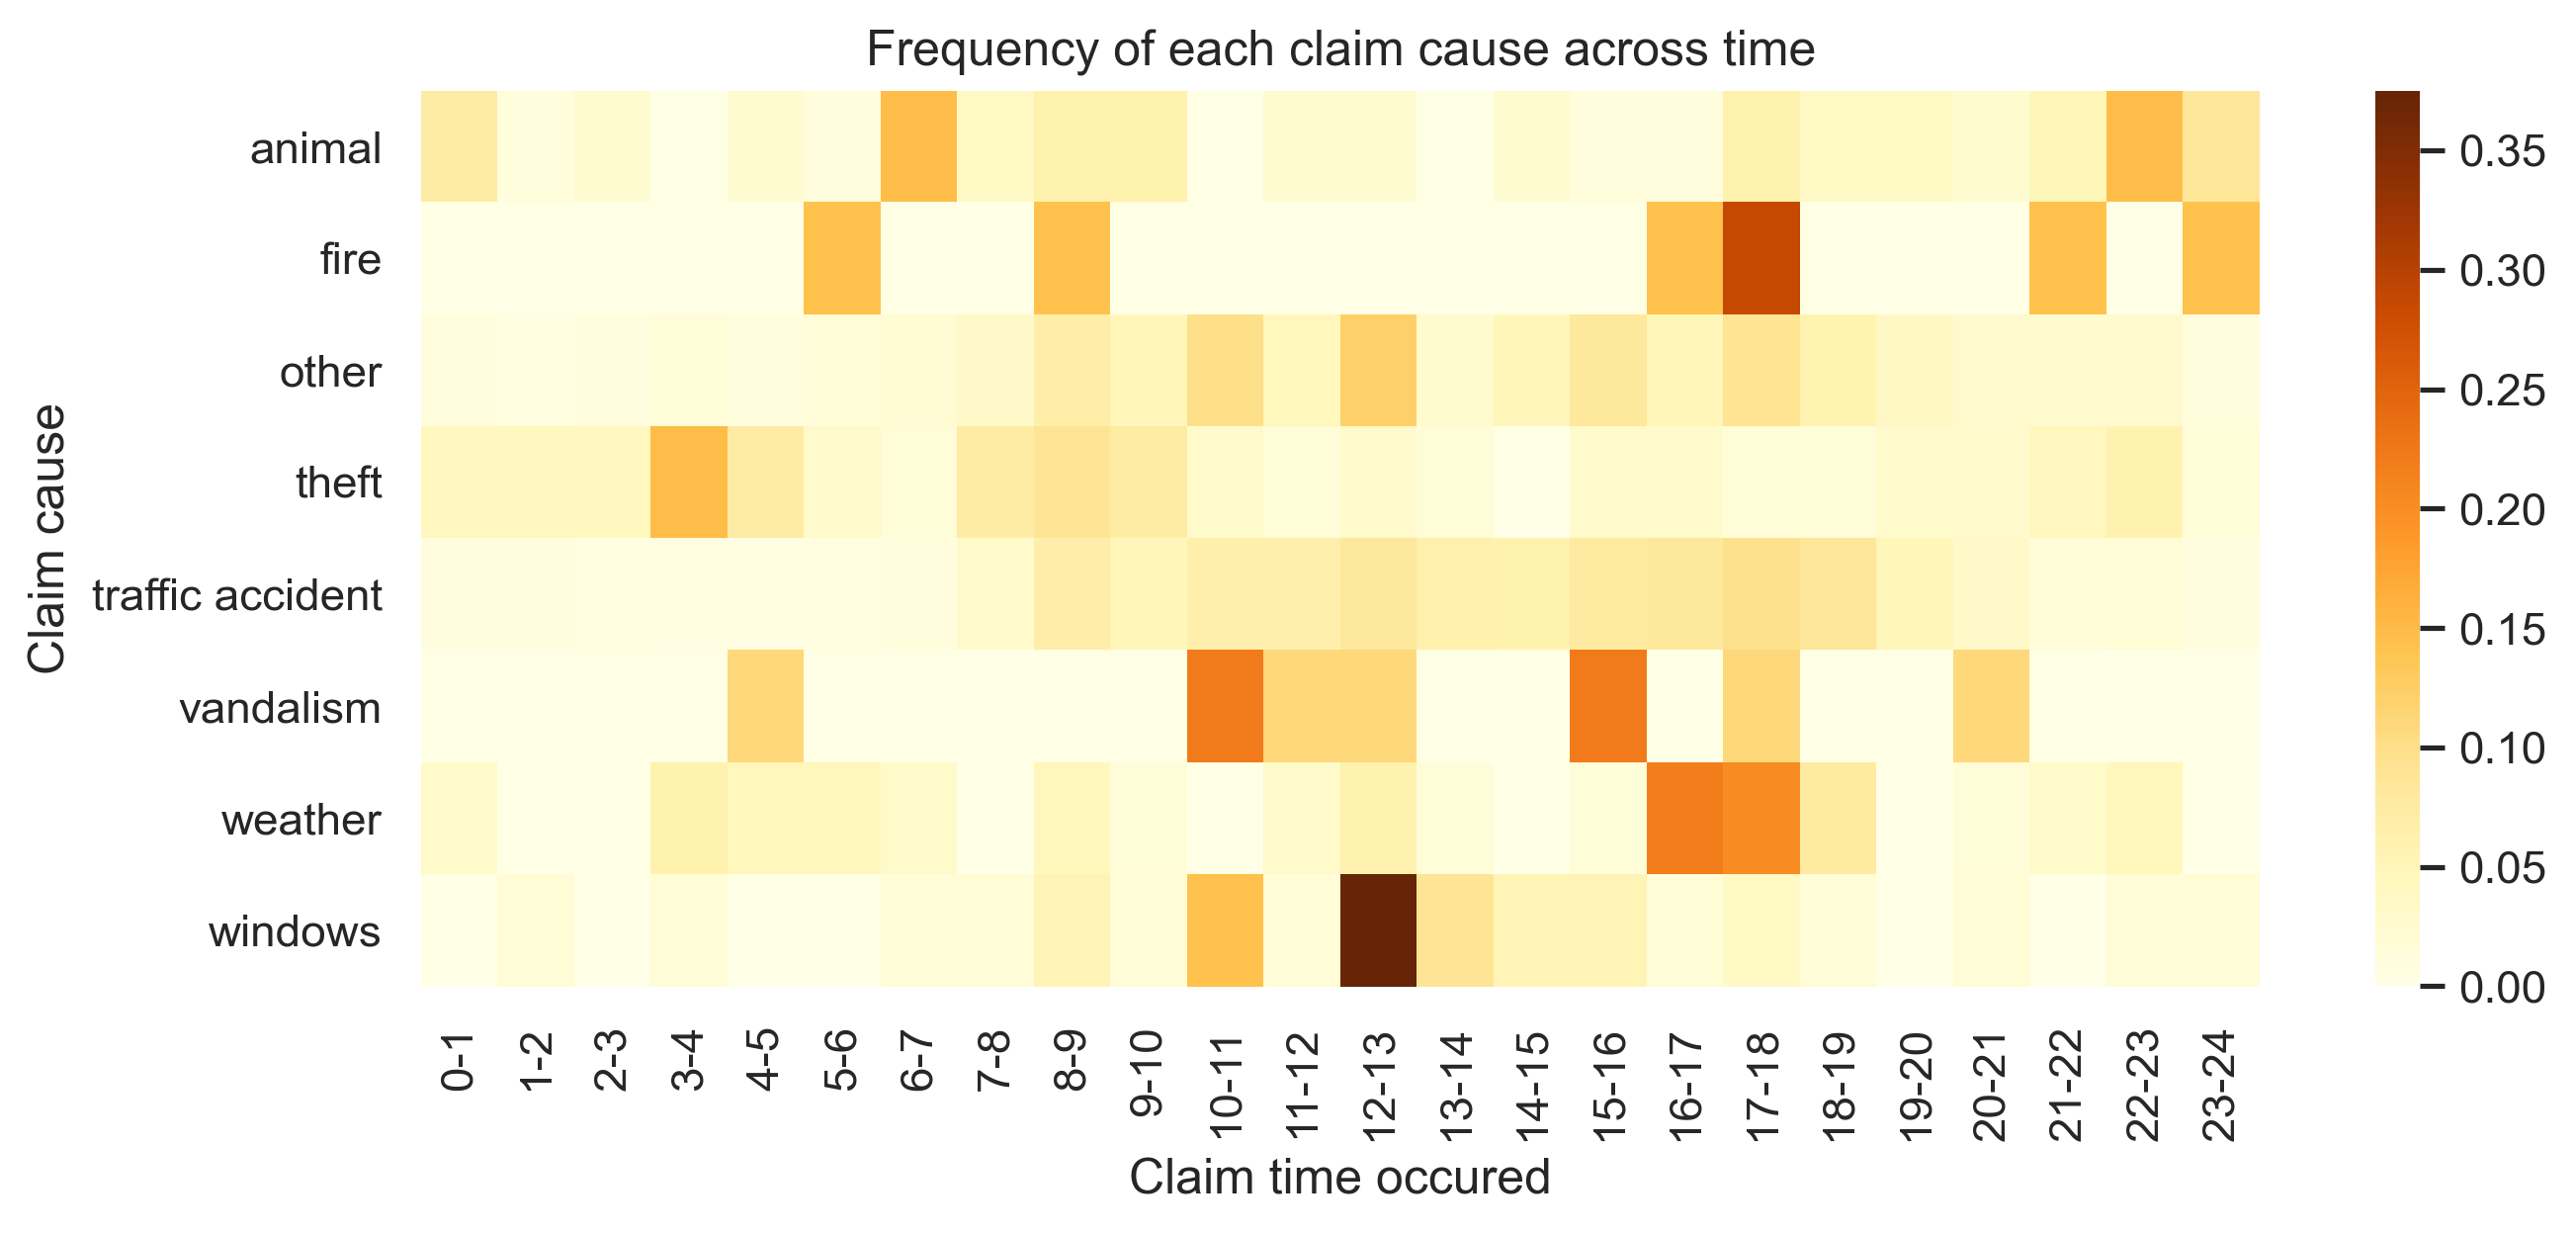
\includegraphics[width = 14cm, height = 7cm]{freq_claim_cause_across_time}
\caption{Frequency of claim causes across time, with missing data excluded}
\end{figure}

\vspace{-0.5cm}
For postal code-related features, as discussed in previous section, postal codes are grouped in terms of their information values from the weight of evidence encoding. The corresponding information values are summarized in figure 15. For \texttt{claim\_postal\_code}, postal codes 7700, 1210 and 6030 have relatively high information values. For \texttt{driver\_postal\_code} and \texttt{policy\_holder\_postal\_code}, postal code 7700 also has the highest information values. It seems that postal code 7700 has some evidence for fraudulent cases. For \texttt{repair\_postal\_code}, postal code 1731 has the highest information value. For \texttt{third\_party\_1\_postal\_code}, \textit{unknown} has the highest information value because fraudulent cases mostly have missing values. For \texttt{third\_party\_2\_postal\_code}, postal code 7141 and 3510 have relatively high information values. For \texttt{third\_party\_3\_postal\_code}, there are no fraudulent cases with non-missing values. Therefore, it is not presented here. 

\begin{figure}[h]
\centering
\begin{subfigure}{.5\textwidth}
  \centering
  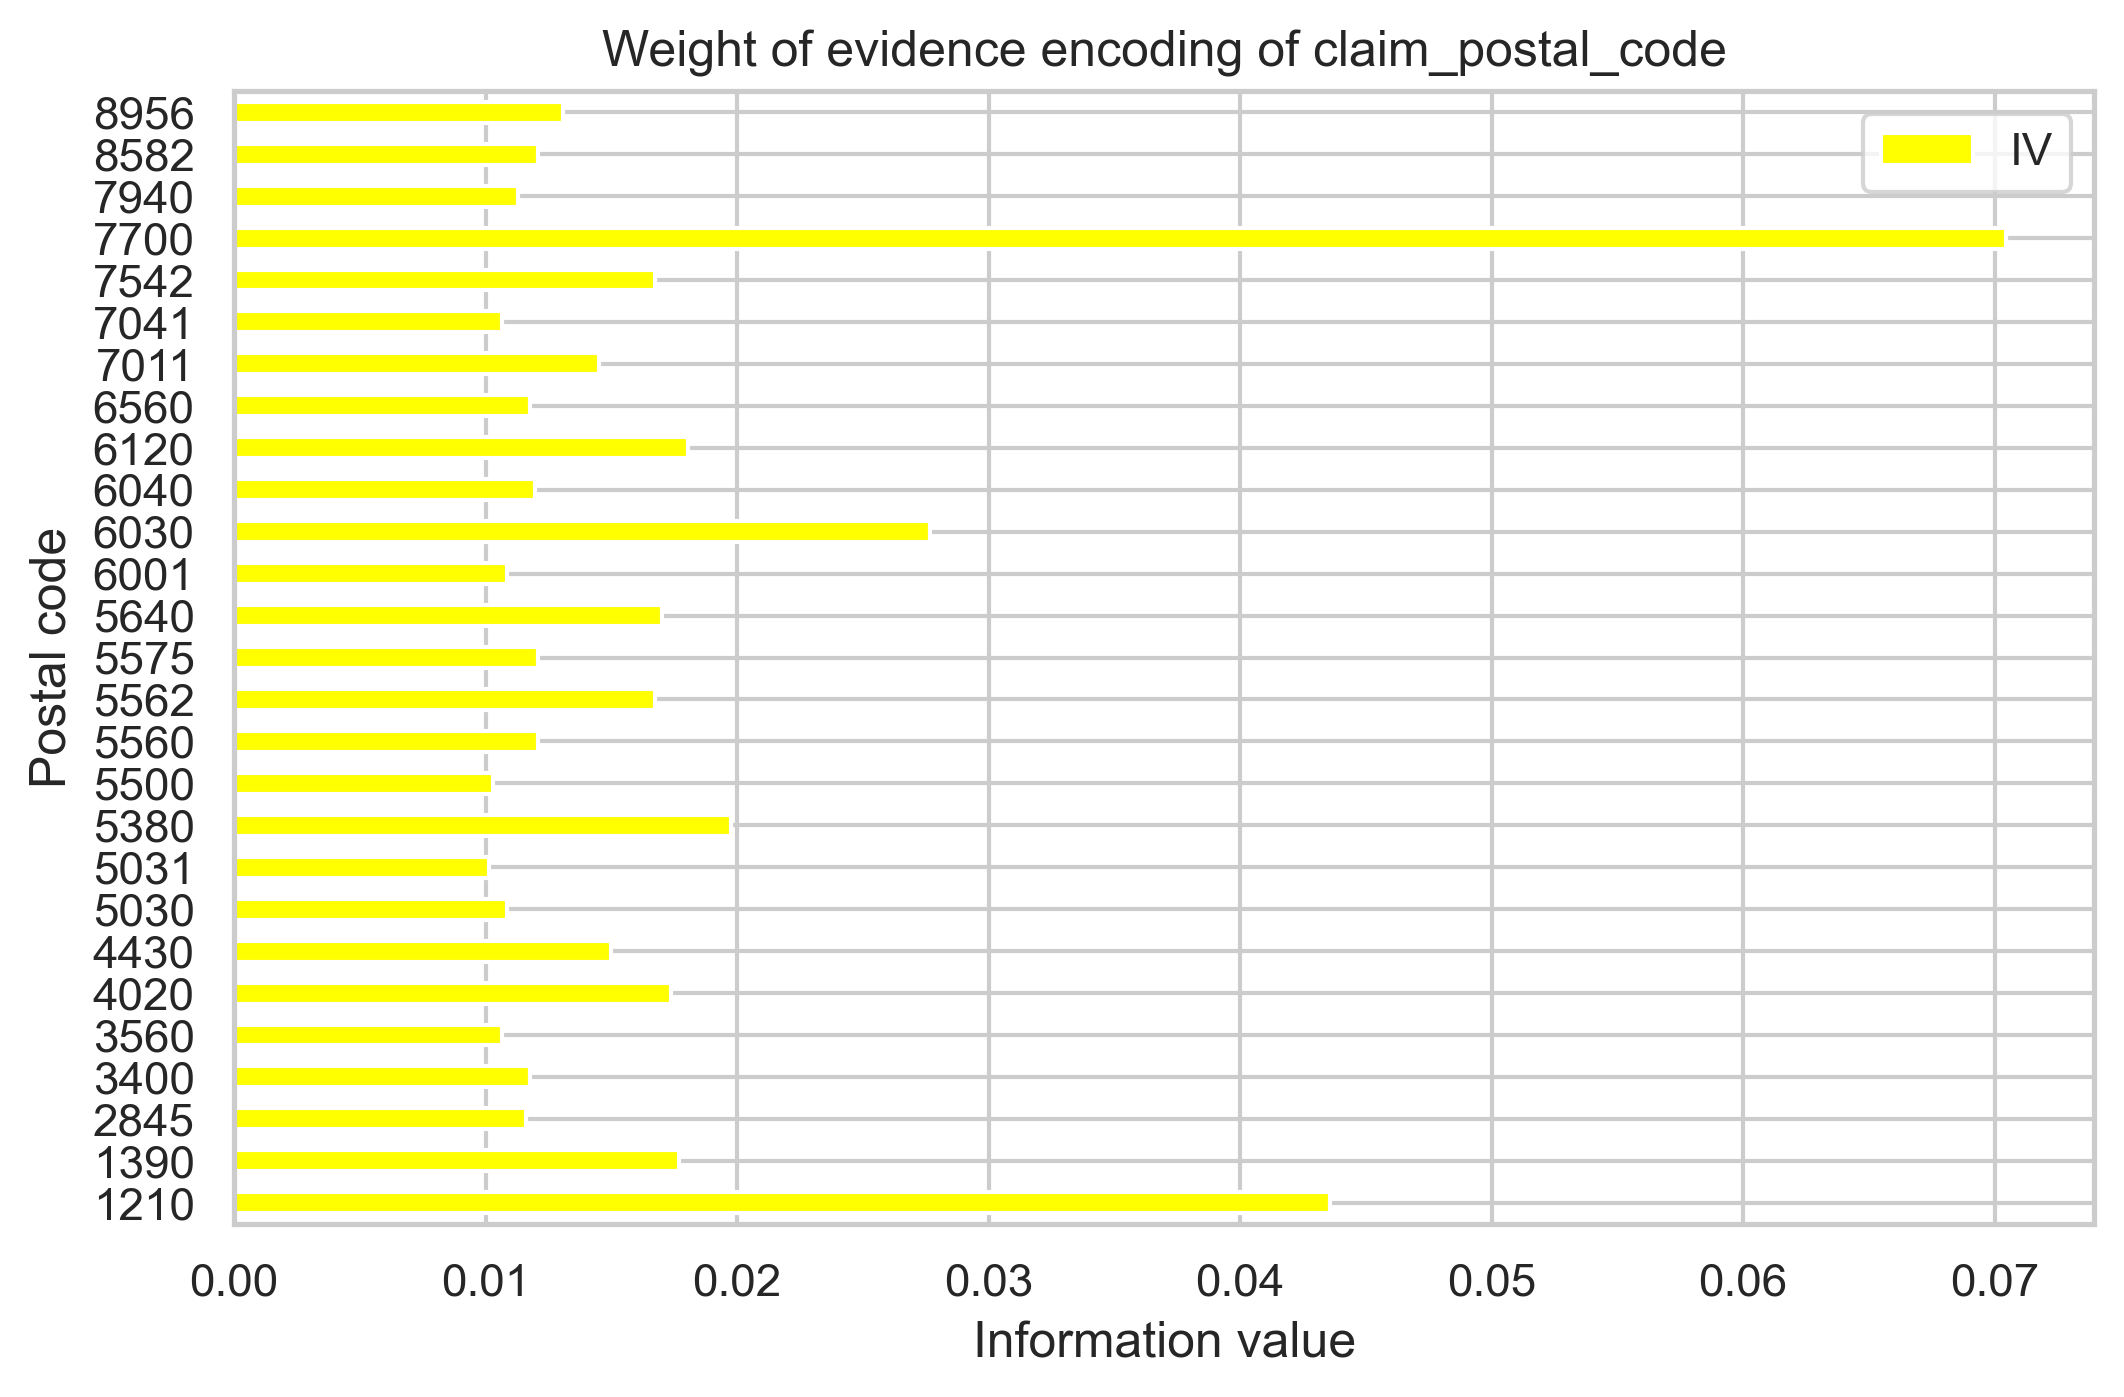
\includegraphics[width=1\linewidth]{info_val_claim_postal_code}
  \caption{\texttt{claim\_postal\_code}}
  \label{fig:sub1}
\end{subfigure}%
\begin{subfigure}{.5\textwidth}
  \centering
  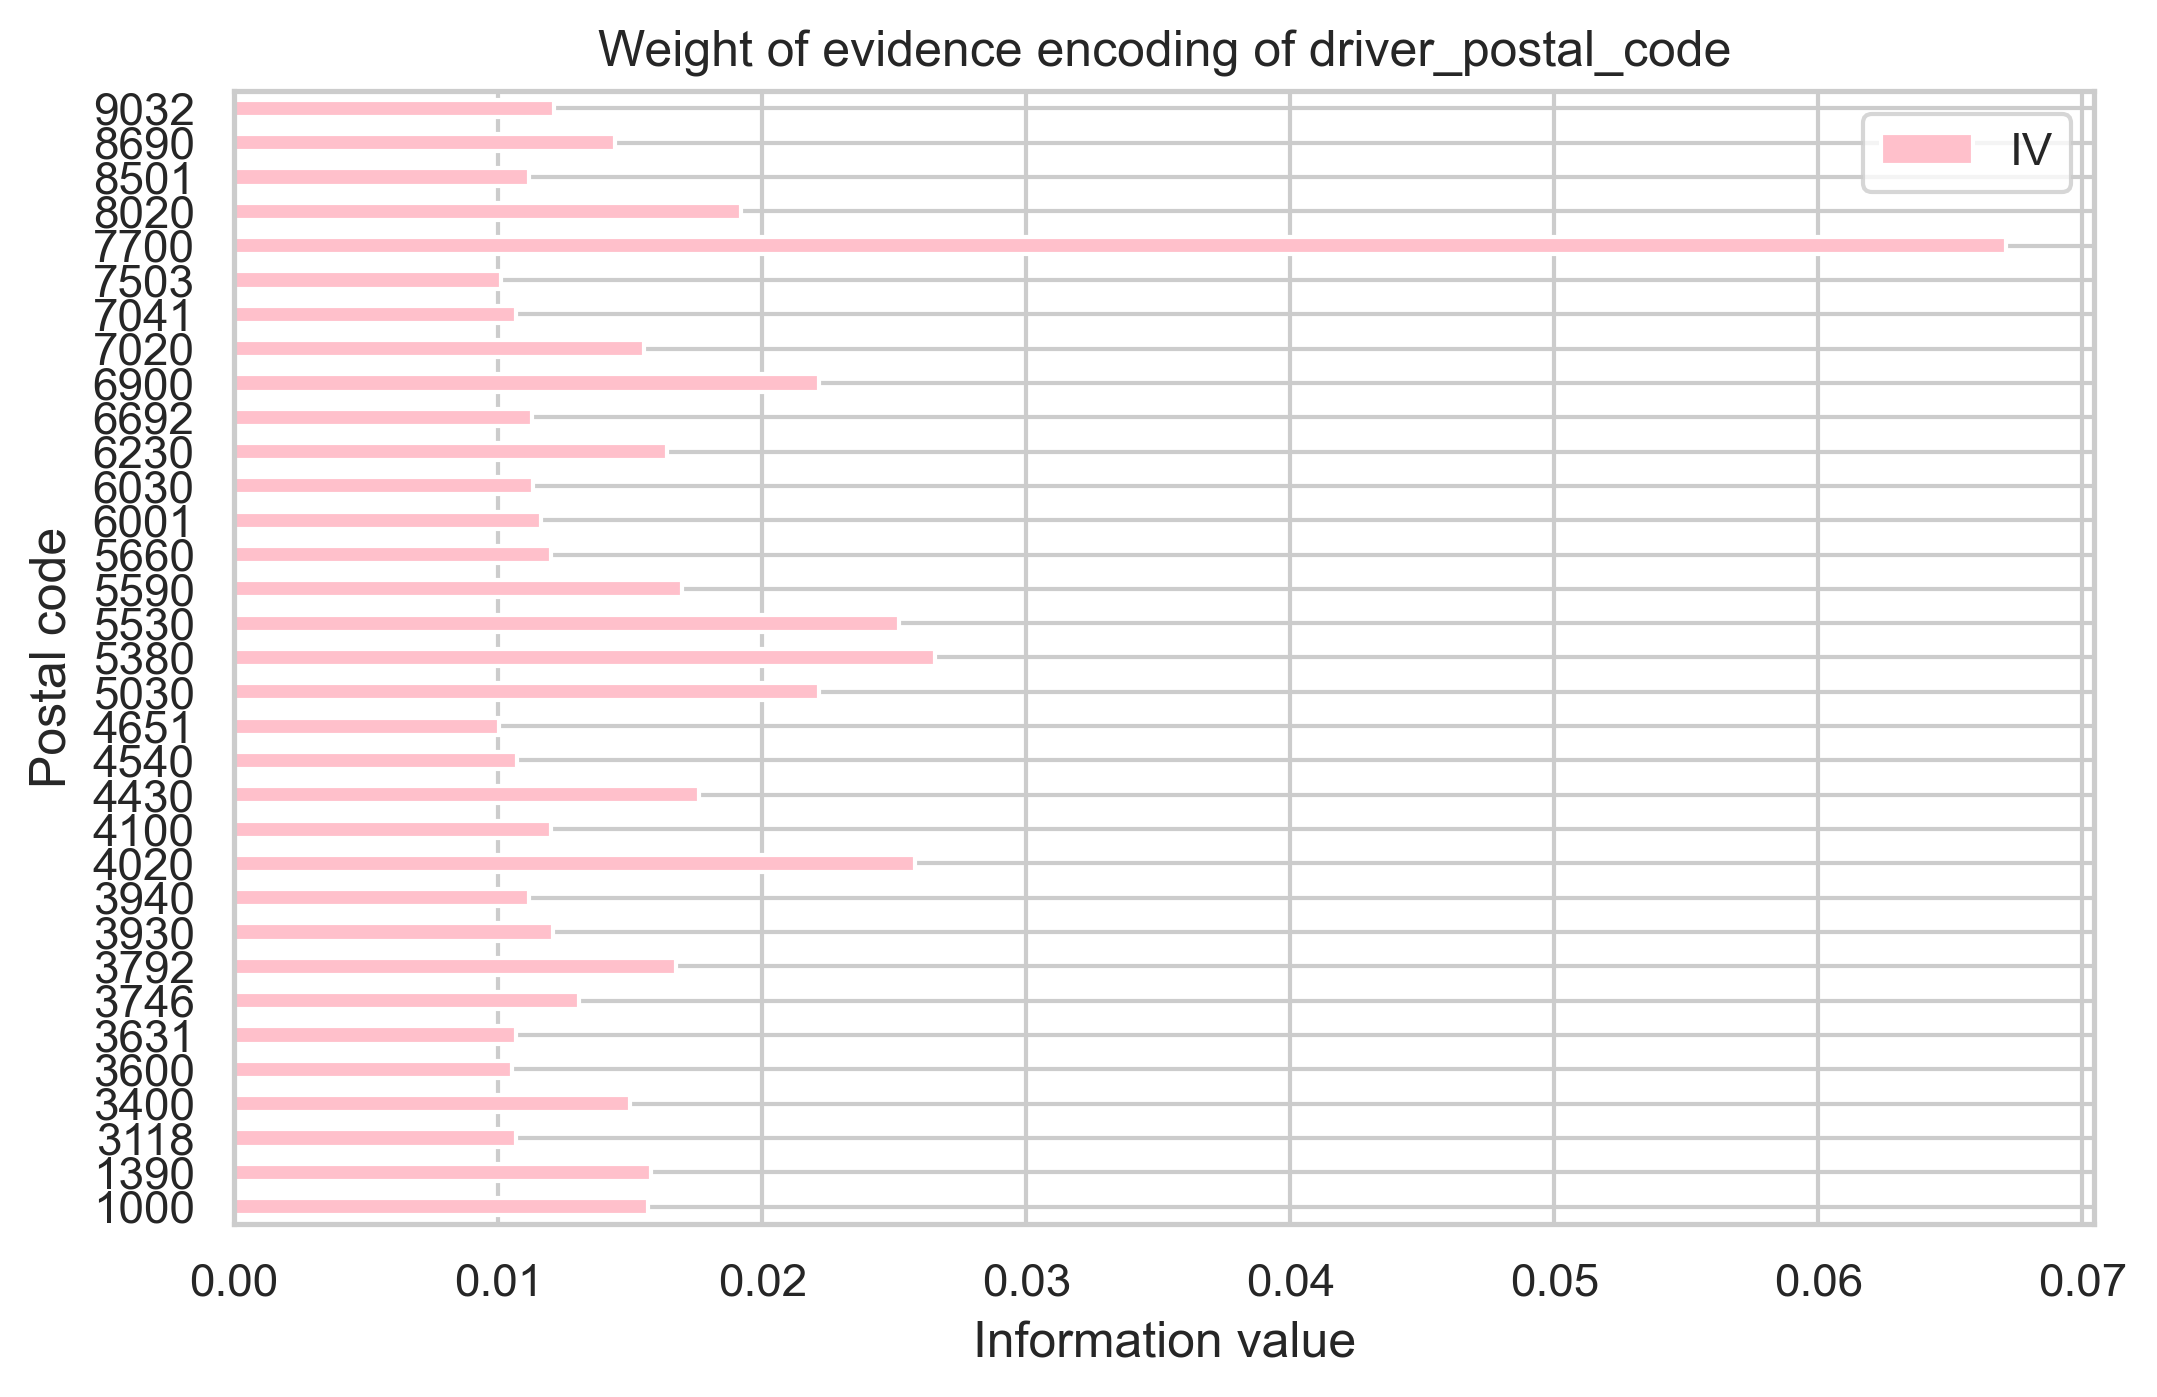
\includegraphics[width=1\linewidth]{info_val_driver_postal_code}
  \caption{\texttt{driver\_postal\_code}}
  \label{fig:sub2}
\end{subfigure}
\vspace{0.5cm}

\begin{subfigure}{.5\textwidth}
  \centering
  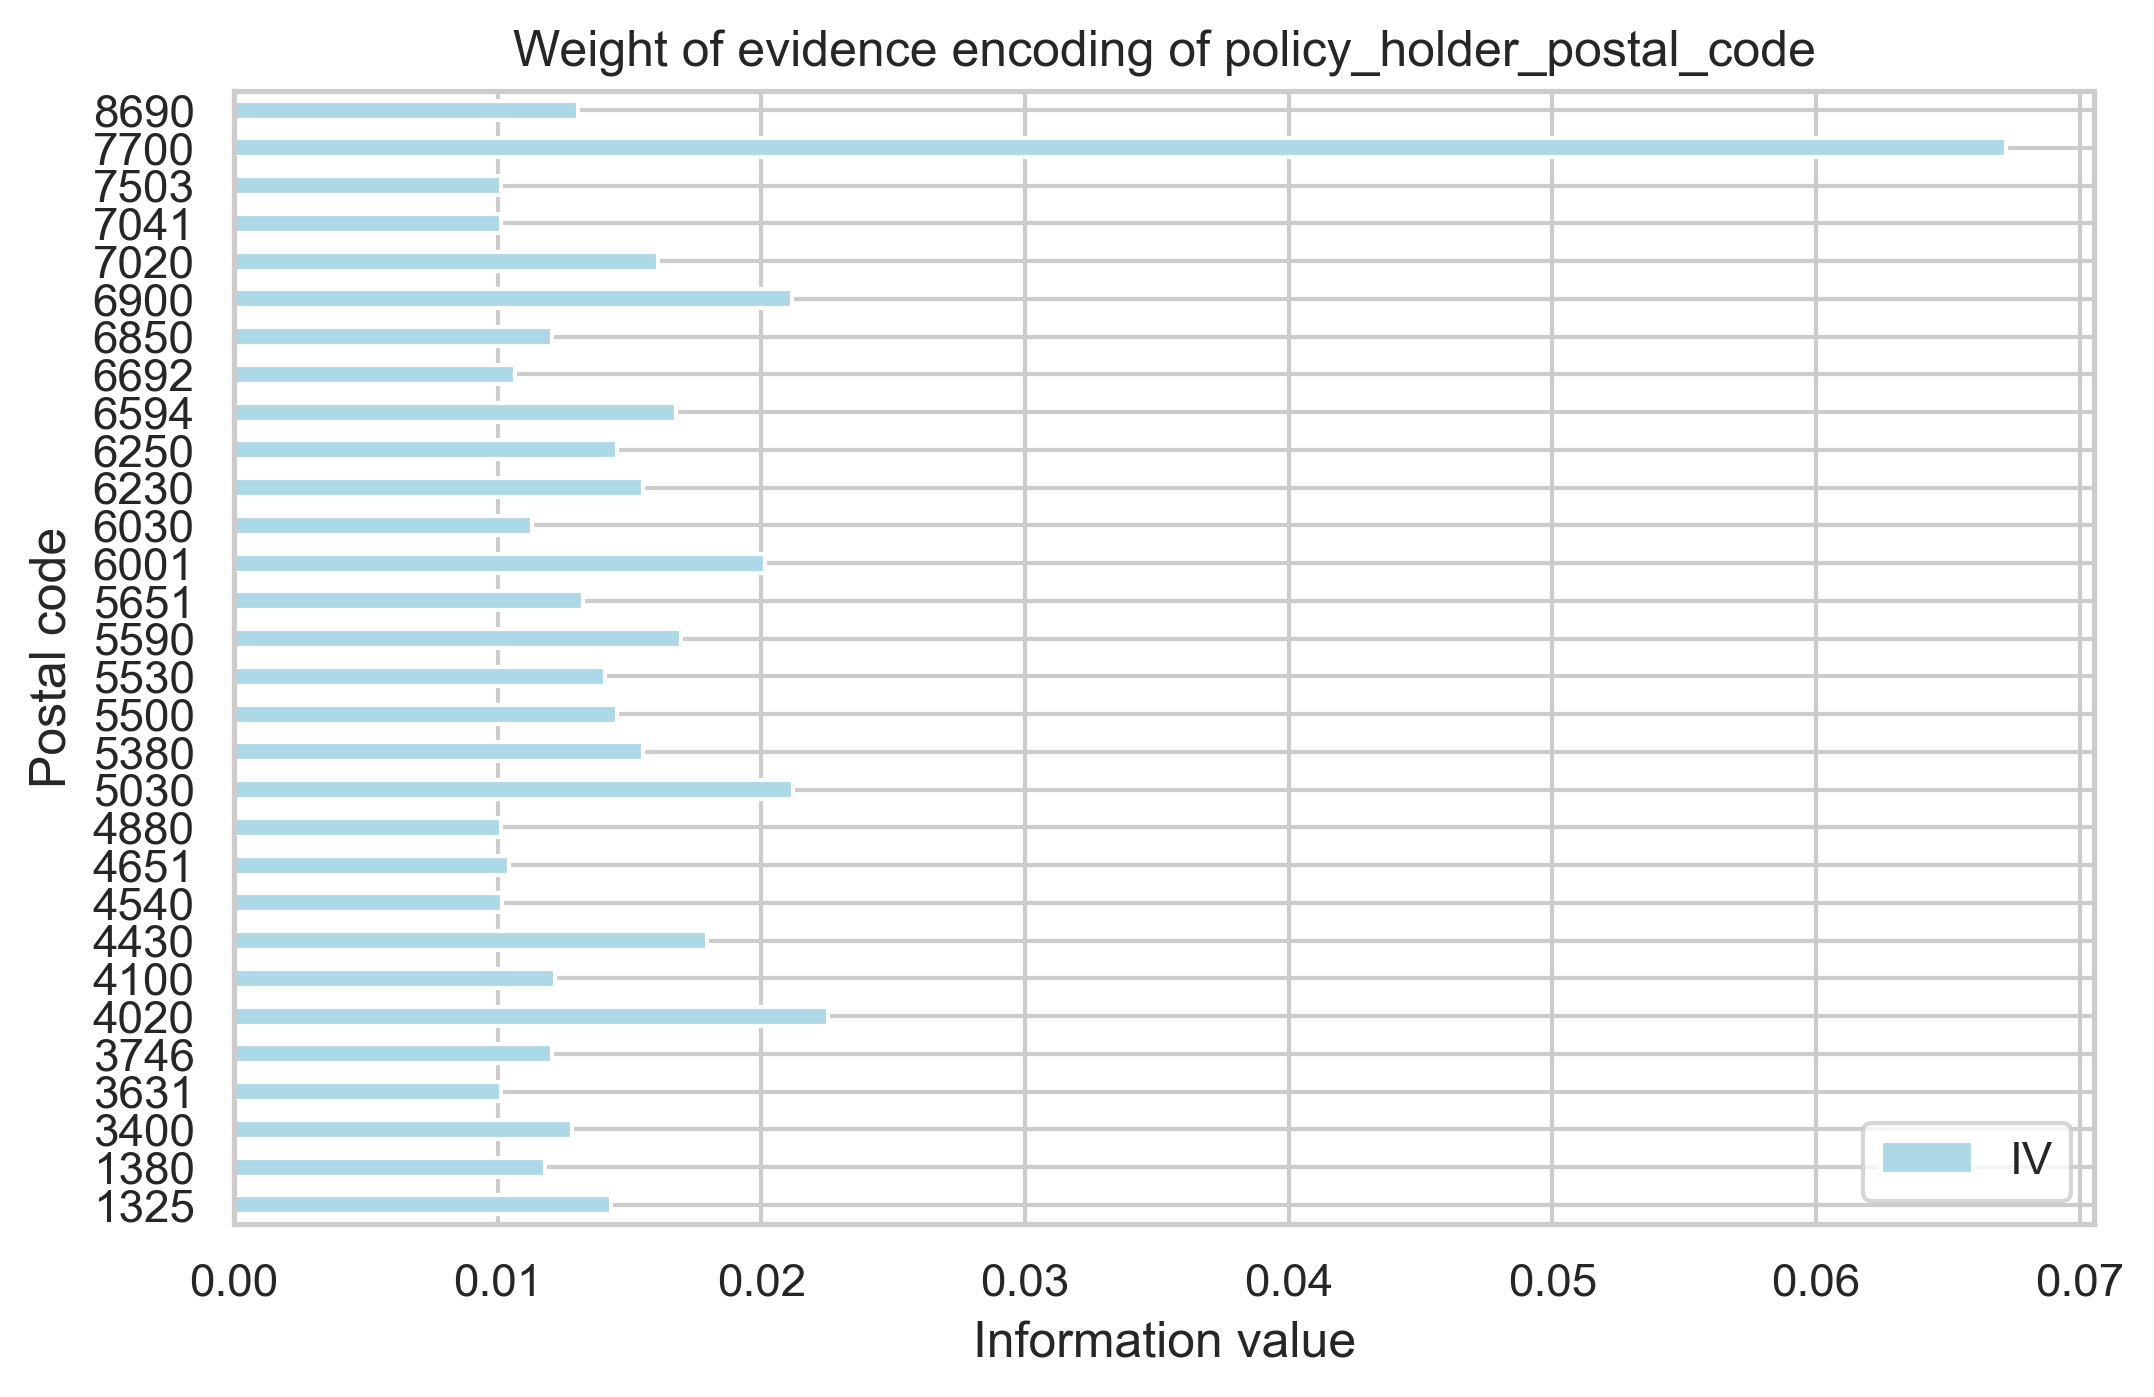
\includegraphics[width=1\linewidth]{info_val_policy_holder_postal_code}
  \caption{\texttt{policy\_holder\_postal\_code}}
  \label{fig:sub3}
\end{subfigure}%
\begin{subfigure}{.5\textwidth}
  \centering
  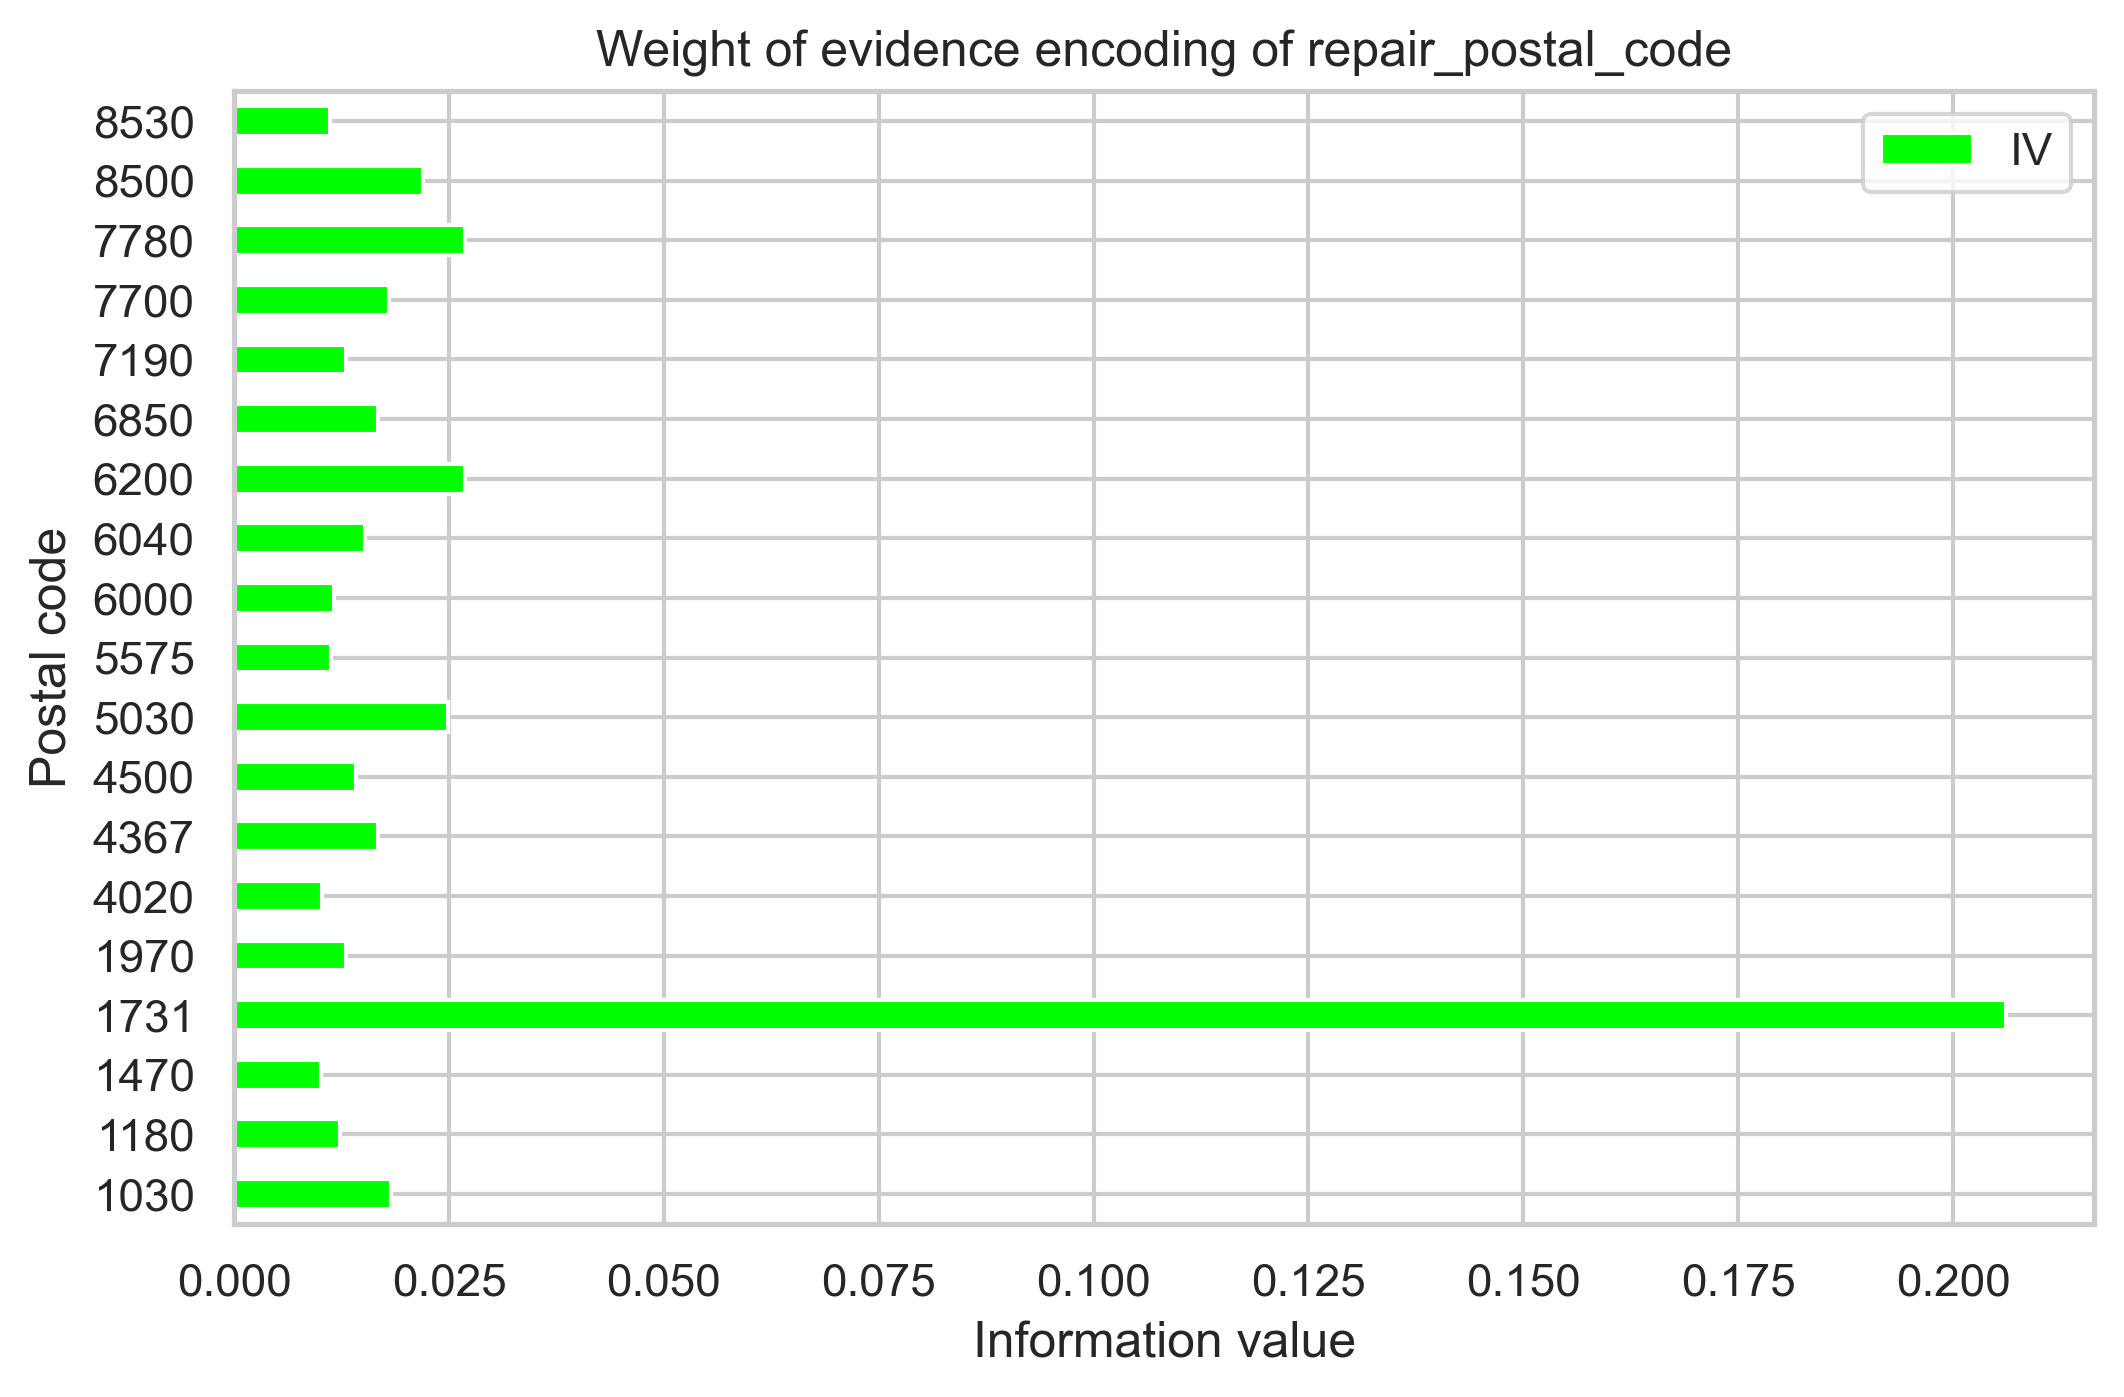
\includegraphics[width=1\linewidth]{info_val_repair_postal_code}
  \caption{\texttt{repair\_postal\_code}}
  \label{fig:sub4}
\end{subfigure}
\vspace{0.5cm}

\begin{subfigure}{.5\textwidth}
  \centering
  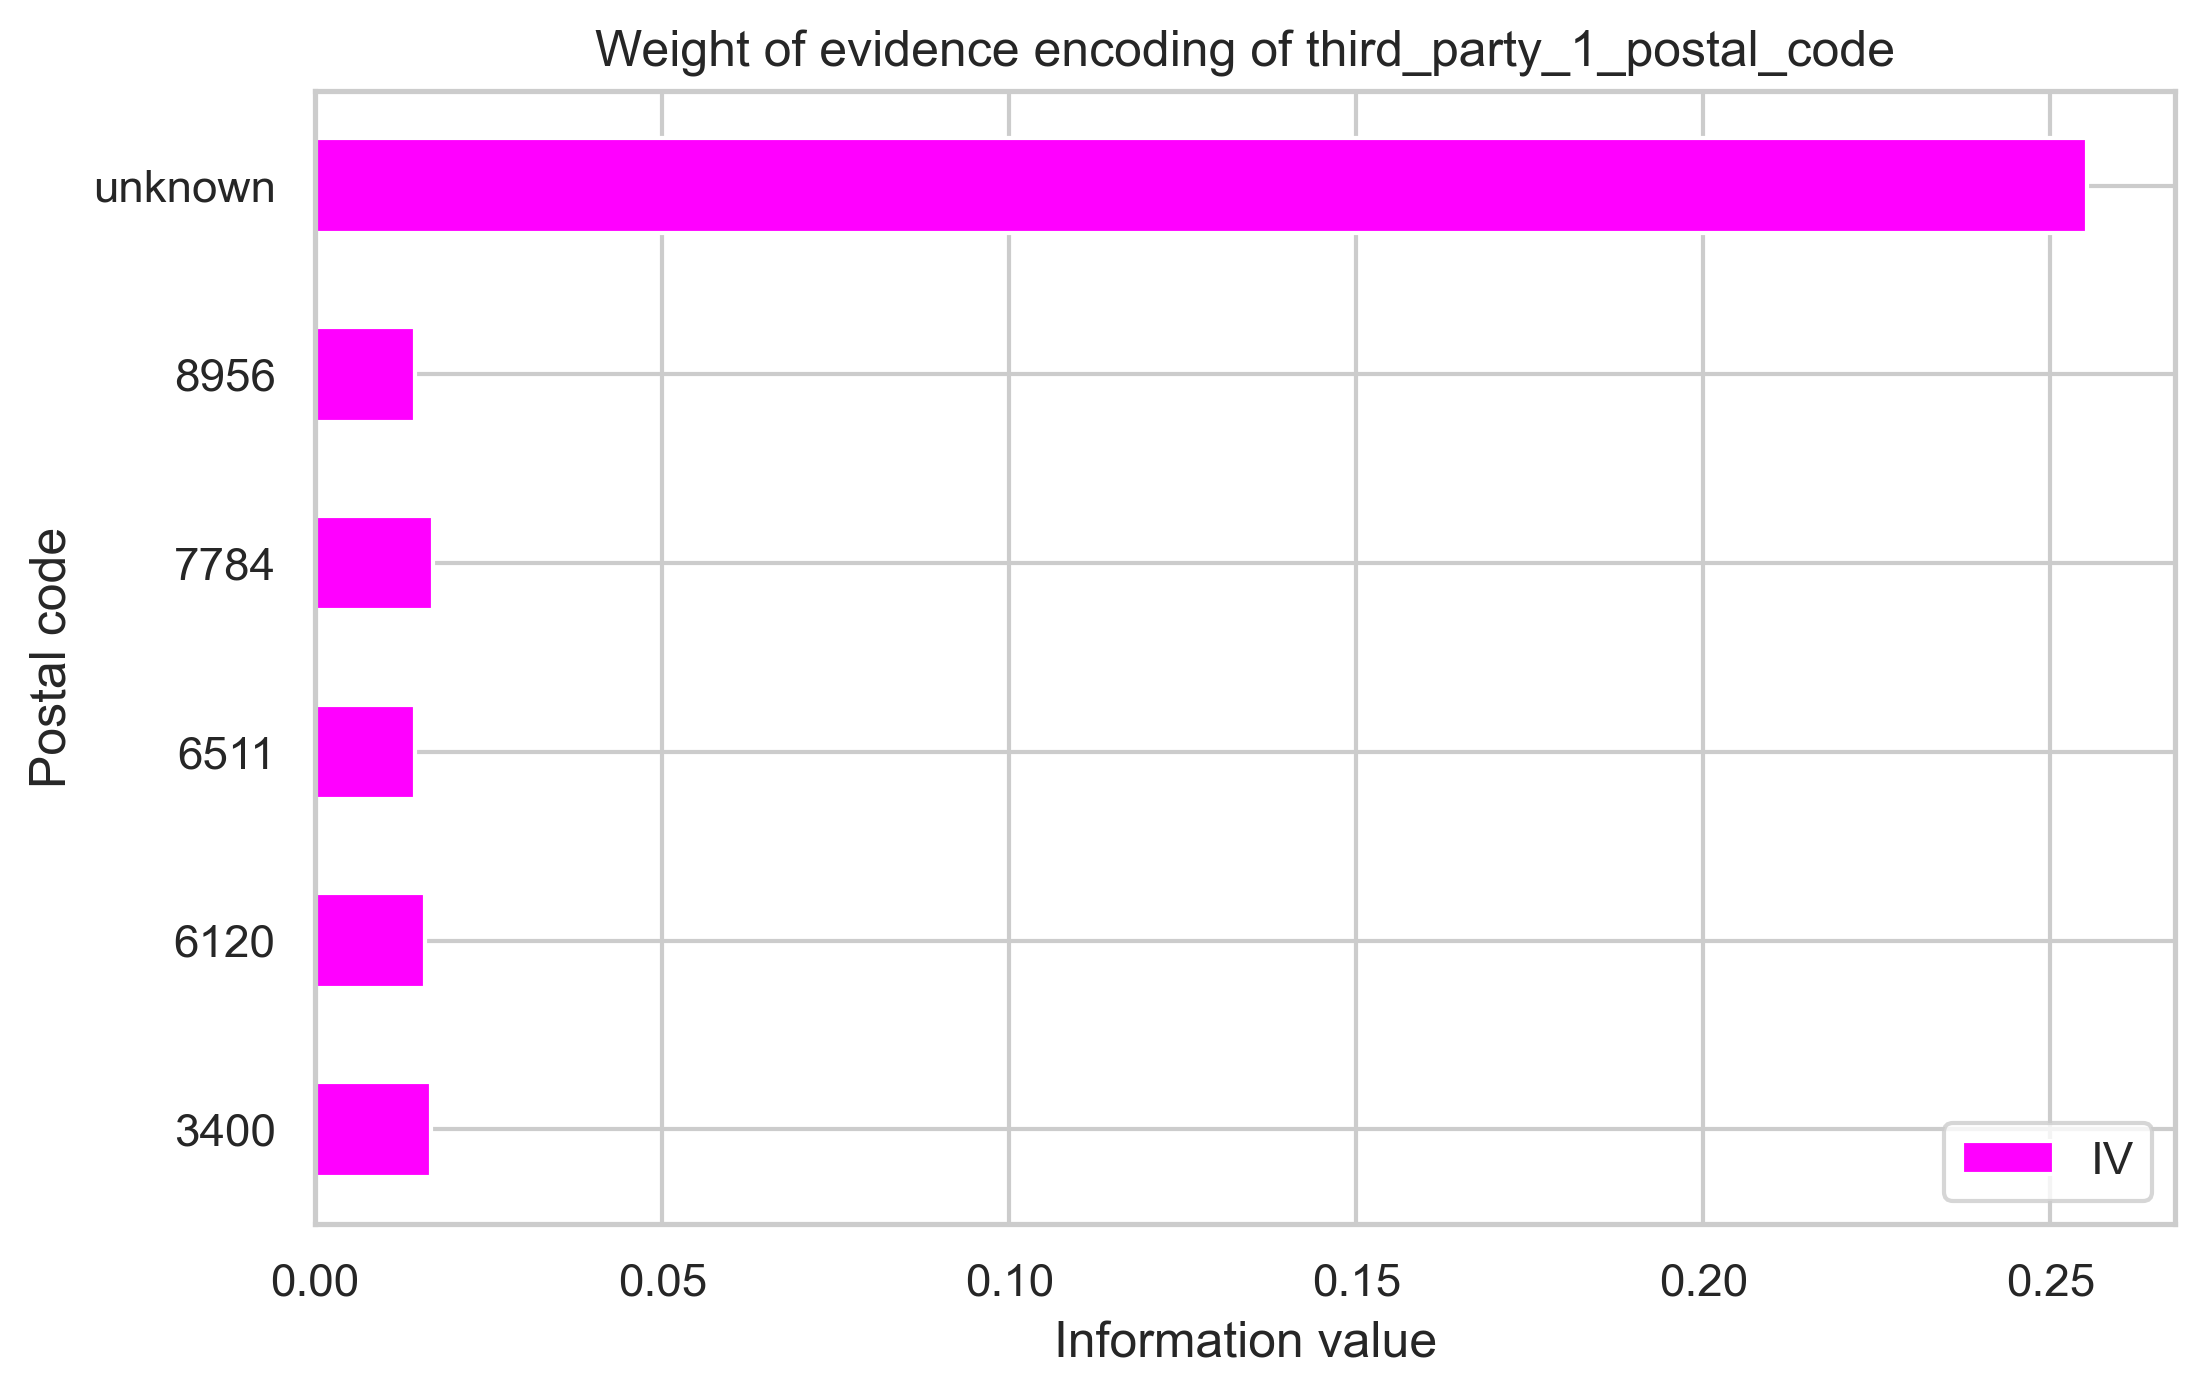
\includegraphics[width=1\linewidth]{info_val_third_party_1_postal_code}
  \caption{\texttt{third\_party\_1\_postal\_code}}
  \label{fig:sub5}
\end{subfigure}%
\begin{subfigure}{.5\textwidth}
  \centering
  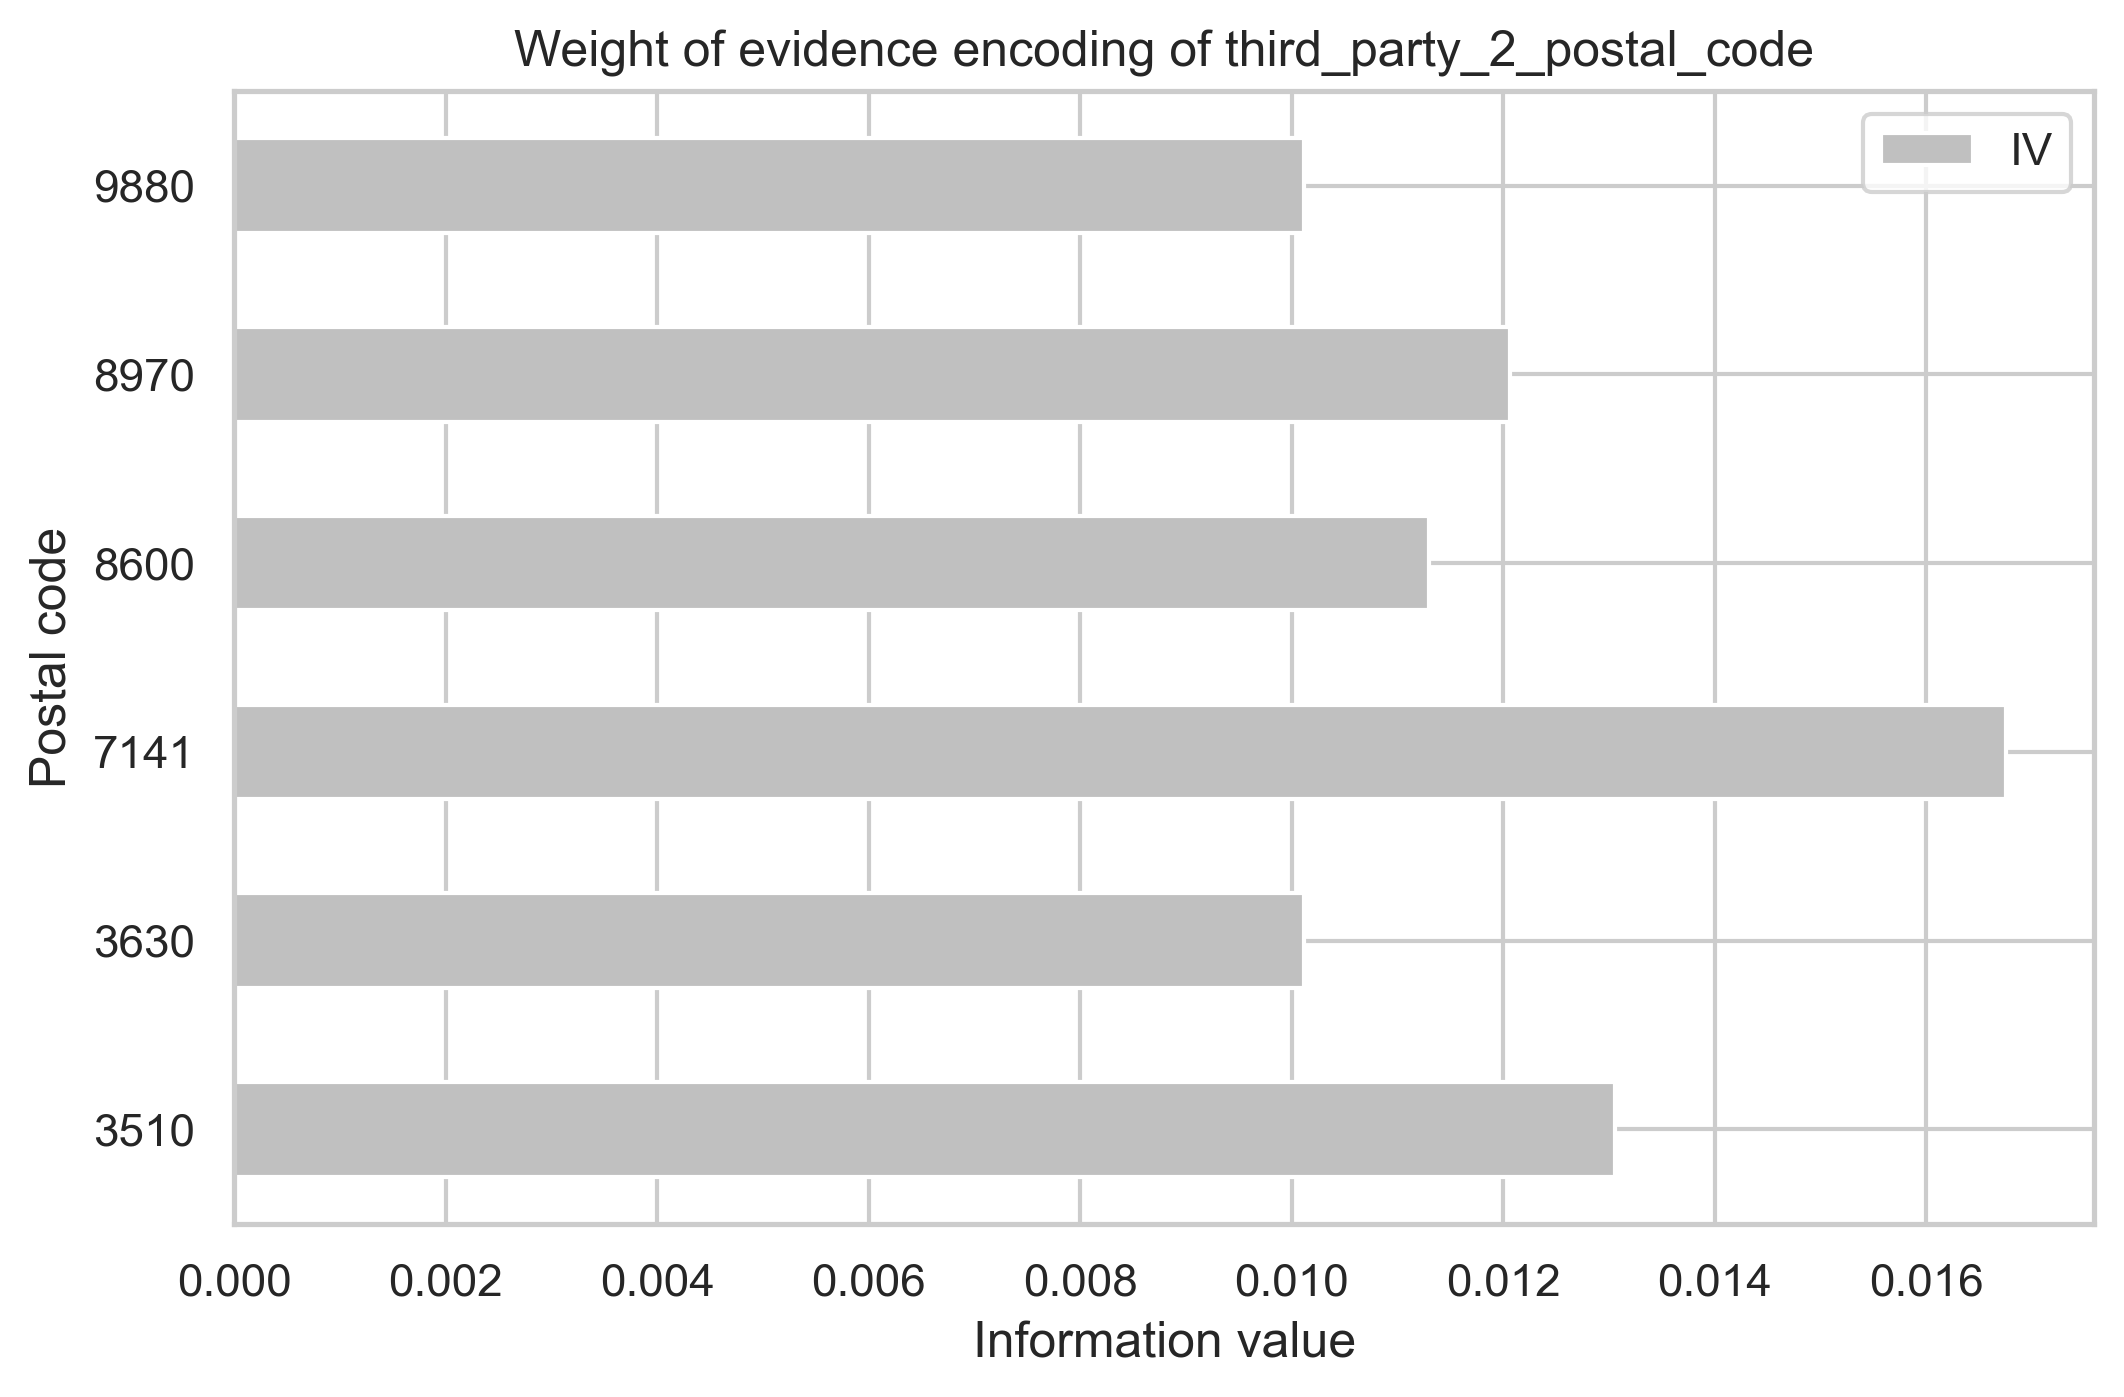
\includegraphics[width=1\linewidth]{info_val_third_party_2_postal_code}
  \caption{\texttt{third\_party\_2\_postal\_code}}
  \label{fig:sub6}
\end{subfigure}
\caption{Information values for postal code-related features}
\label{fig:iv_postal_code}
\end{figure}

\clearpage

There are 73 different policy coverage types in total. After weight of evidence encoding, coverage types \#000110000, \#111110001 and \#000110100 show relatively high information values as shown in figure 16. These coverage types may be informative in identifying fraudulent cases.

\begin{figure}[h]
\centering
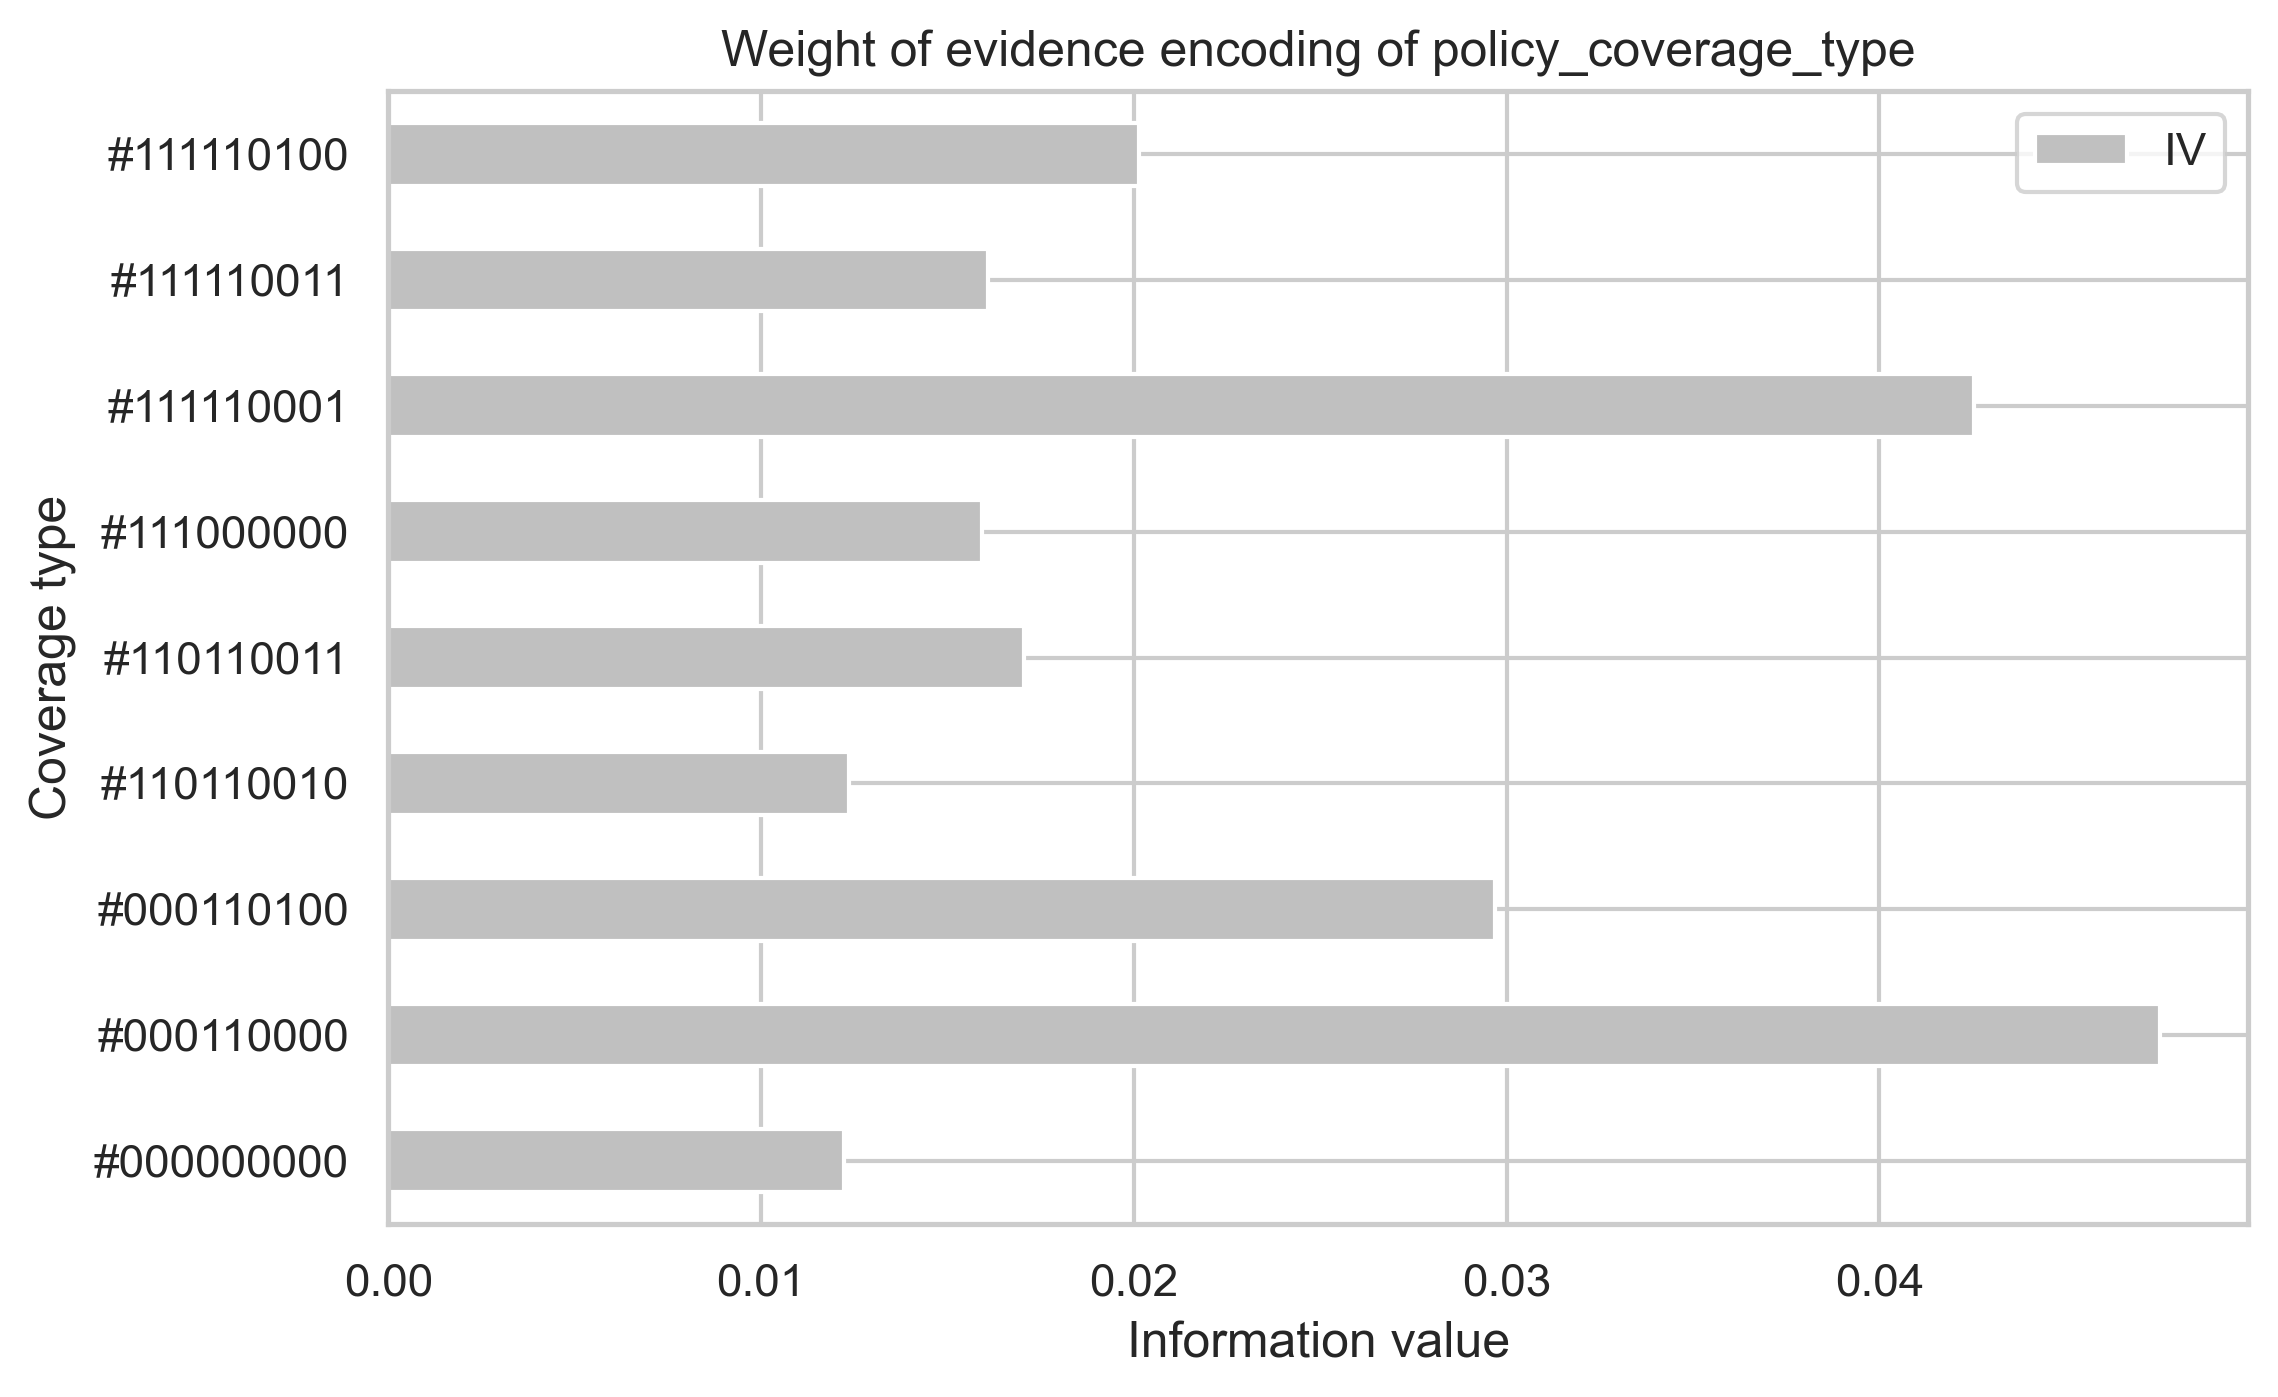
\includegraphics[width = 10cm, height = 7cm]{info_val_policy_coverage_type}
\caption{Information values for policy coverage types}
\end{figure}


\vspace{-0.5cm}
\subsubsection*{Correlation plot}
\addcontentsline{toc}{subsubsection}{Correlation plot}

High correlation among features may indicate the existence of some redundant features. Therefore, a correlation plot is presented in figure 17, and we observe that the correlation among \texttt{policy\_coverage\_1000} and \texttt{claim\_vehicle\_cyl} and \texttt{claim\_vehicle\_power} are strong. And the correlation between \texttt{driver\_age} and \texttt{policy\_holder\_age} are also strong. There may be some common factors behind correlated features. Although the correlations are strong. Instead of dropping them, we can discretize the features to reduce the correlation and preserve information as they are not 100\% correlated. As discussed in previous section, age-related features are discretized. Moreover, we discretize \texttt{policy\_coverage\_1000} into equal intervals because it has more than 50\% of missing values and a strong correlation.


\subsubsection*{Dimension reduction}
\addcontentsline{toc}{subsubsection}{Dimension reduction}

For exploratory analysis, we visualize the training data using dimension reduction techniques. Uniform manifold approximation and projection (Umap) is a dimension reduction technique using manifold learning, which efficiently embeds or represents the topology of higher dimension space with a lower dimension space through approximation. Of course, there are many other popular dimension reduction techniques available like t-distributed stochastic neighbor embedding (tSNE) and principal component analysis (PCA) and its variants e.g. kernel PCA. However, it is hard to incorporate class label using tSNE, whereas Umap supports supervised dimension reduction. Moreover, Umap tends to give a more stable results and preserves more global structure compared to tSNE. \\

For PCA which reduces dimensions in a linear fashion, the correlation plot in mentioned in the previous subsection shows most of the features do not share a high linear correlation. Thus, eigendecomposition on covariance matrix would not reduce much dimensions as expected. In this sense, Umap is an appealing tool for dimension reduction. In this section, we use \texttt{umap-learn} python library to perform Umap.

\begin{figure}[h]
\centering
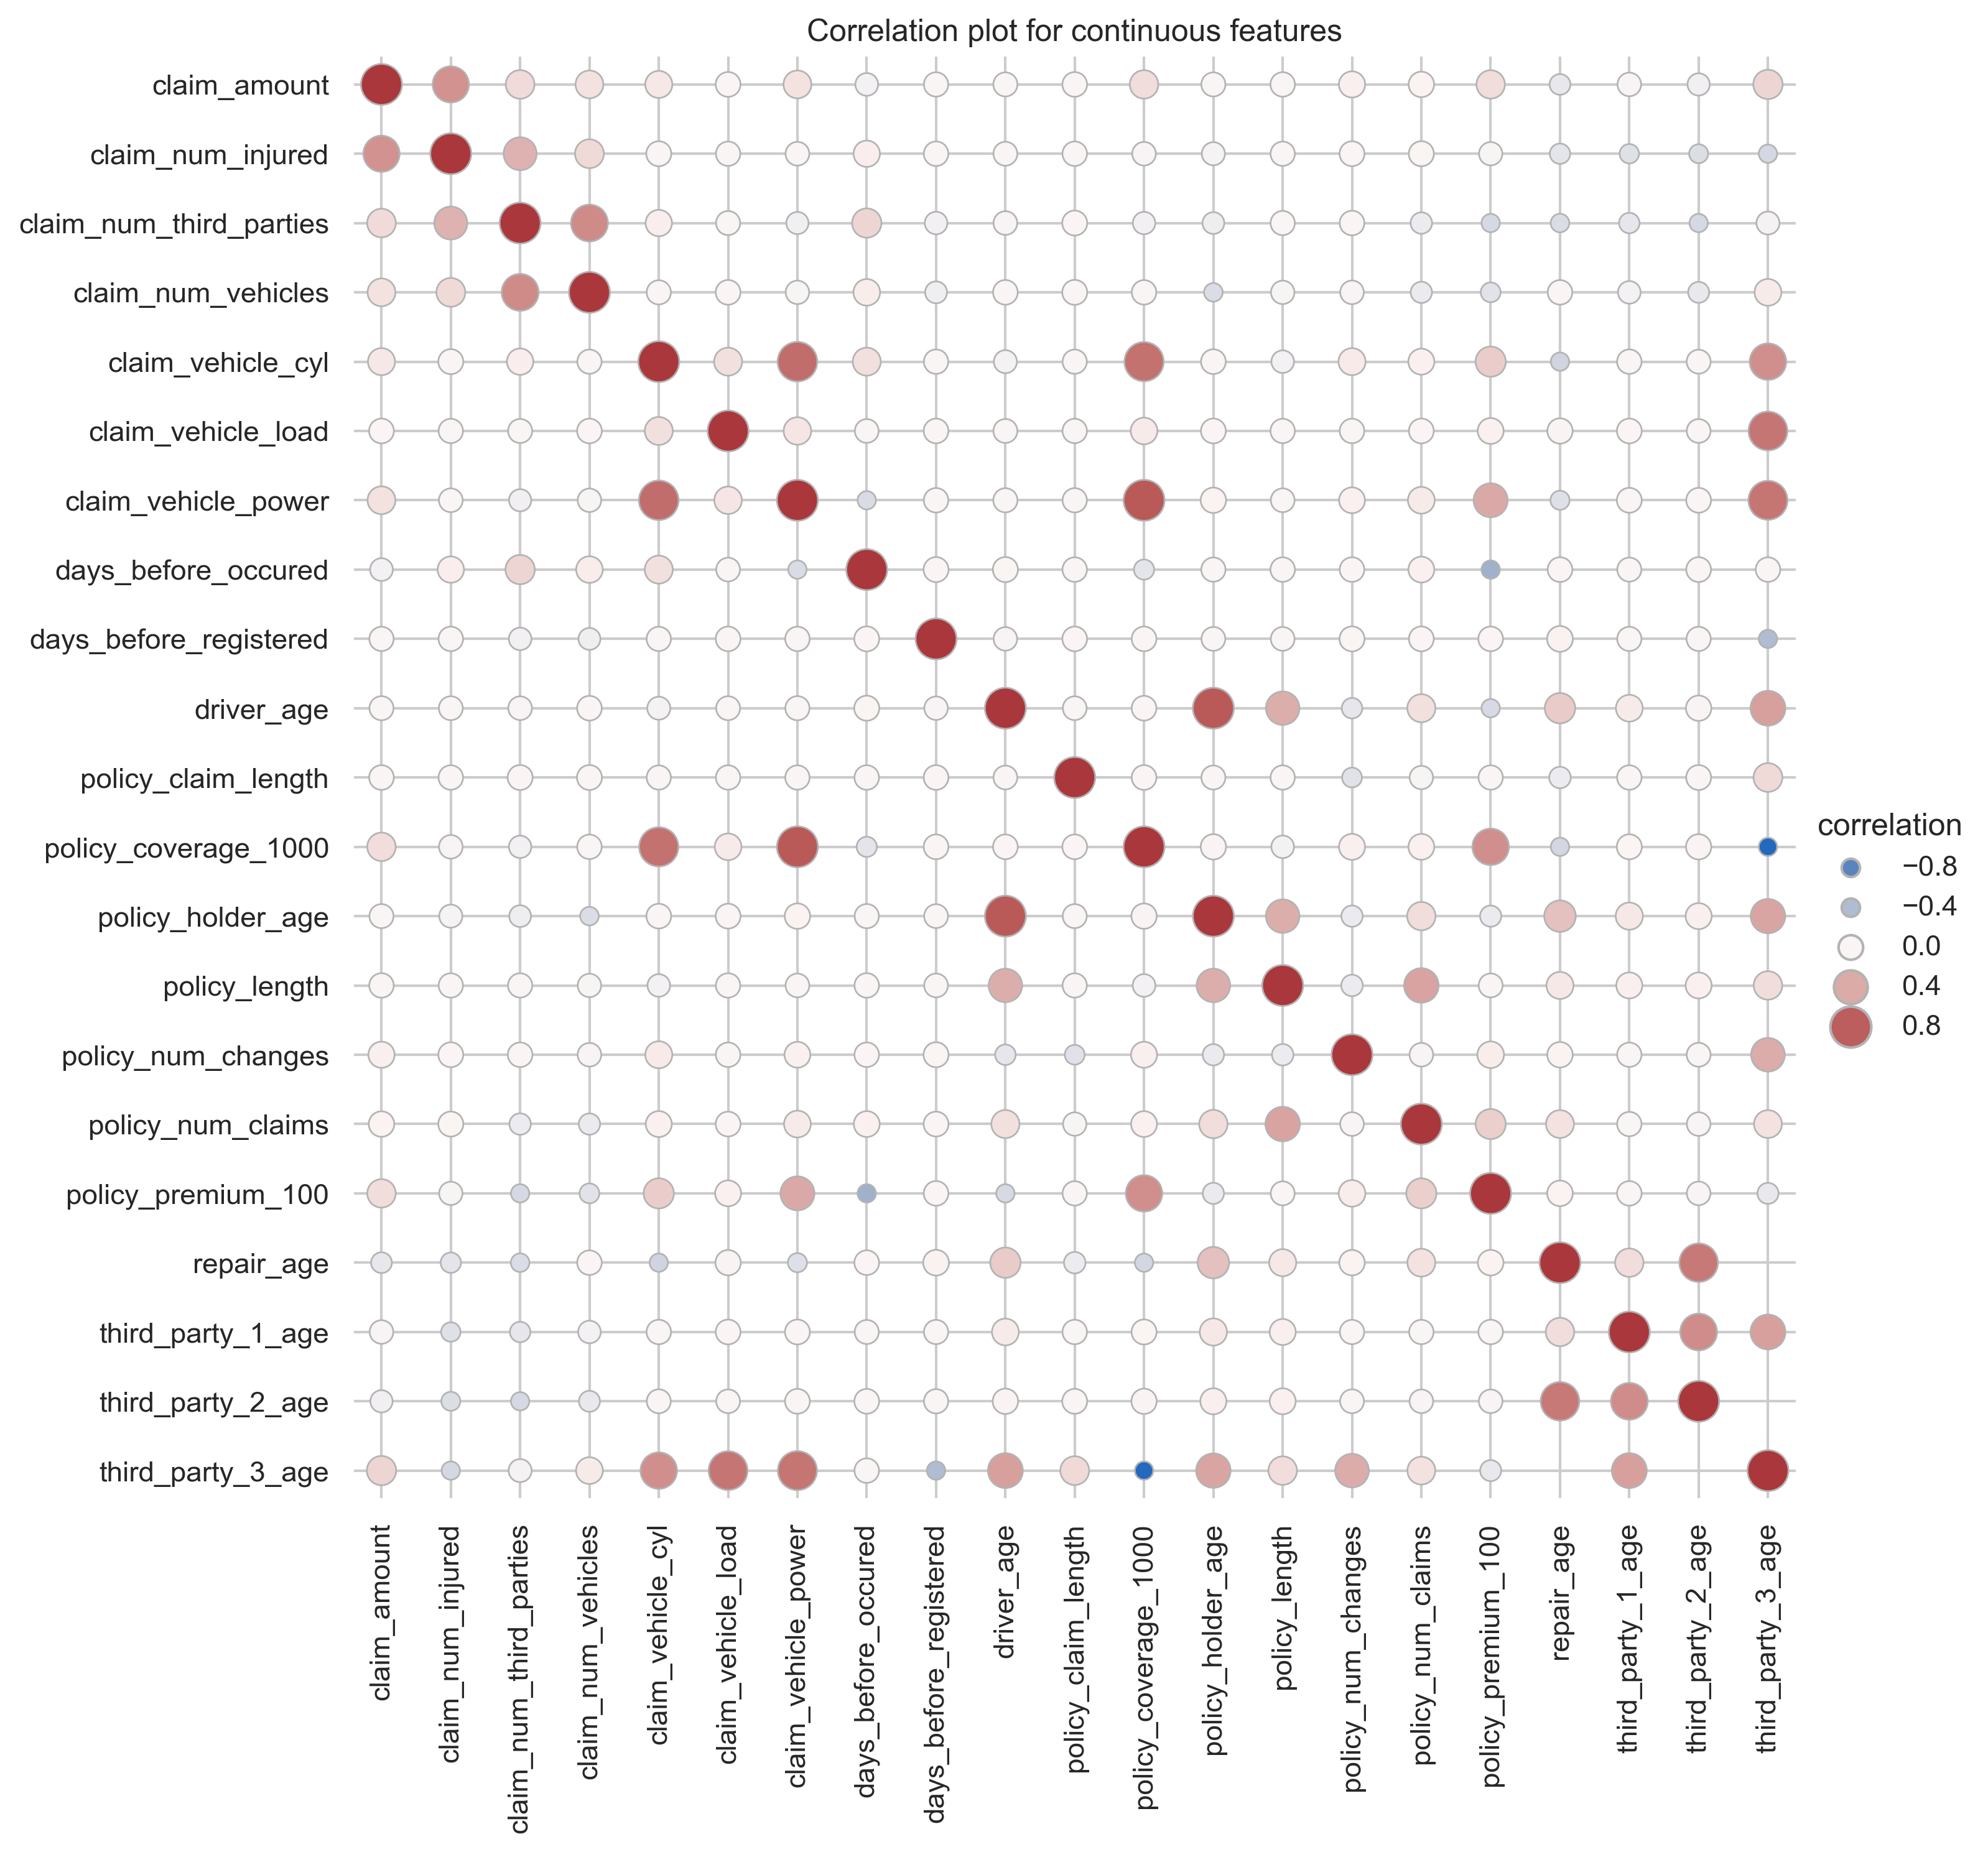
\includegraphics[width = 14cm, height = 12cm]{corr_plot}
\caption{Correlation plot for continuous features}
\end{figure}

\newpage 
There are some hyperparameters in Umap, and the most important hyperparameters are \texttt{n\_components}, \texttt{n\_neighbors}, \texttt{min\_dist} and \texttt{metric}. We notice that \texttt{n\_components} represents the output dimension, usually between 2 and 3 for visualization purpose, while \texttt{n\_neighbors} represents the number of neighbourhood instances used in manifold approximation. The minimum distance among points in the output dimension is controlled by \texttt{min\_dist}. A larger \texttt{min\_dist} would give a more disperse representation in the embedded space. The distance metric defined between two points in original dimensional space is controlled by \texttt{metric} for which the Euclidean distance is applied to continuous features and the Jaccard distance is applied to categorical features after encoding into dummy variables.\\

Outline of the steps in performing dimension reduction:

\begin{enumerate}

\item Apply featurization and imputation to the training data.

\item Standardize continuous features.

\item Oversampling with SMOTE (due to imbalanced class) from \texttt{imblearn}.

\item Apply Umap to continuous features with the Euclidean distance and to categorical features with the Hamming distance after encoding into dummy variables. 

\item Train Umap with different \texttt{n\_neighbors} and \texttt{min\_dist}.

\end{enumerate}

The results of Umap with difference \texttt{n\_neighbors} are shown in figure 18 and 19. The embedded results for continuous features changes when \texttt{n\_neighbors} increases from 15 to 30, and not much change in the results for categorical features.

\begin{figure}[h]
\centering
\begin{subfigure}{.5\textwidth}
  \centering
  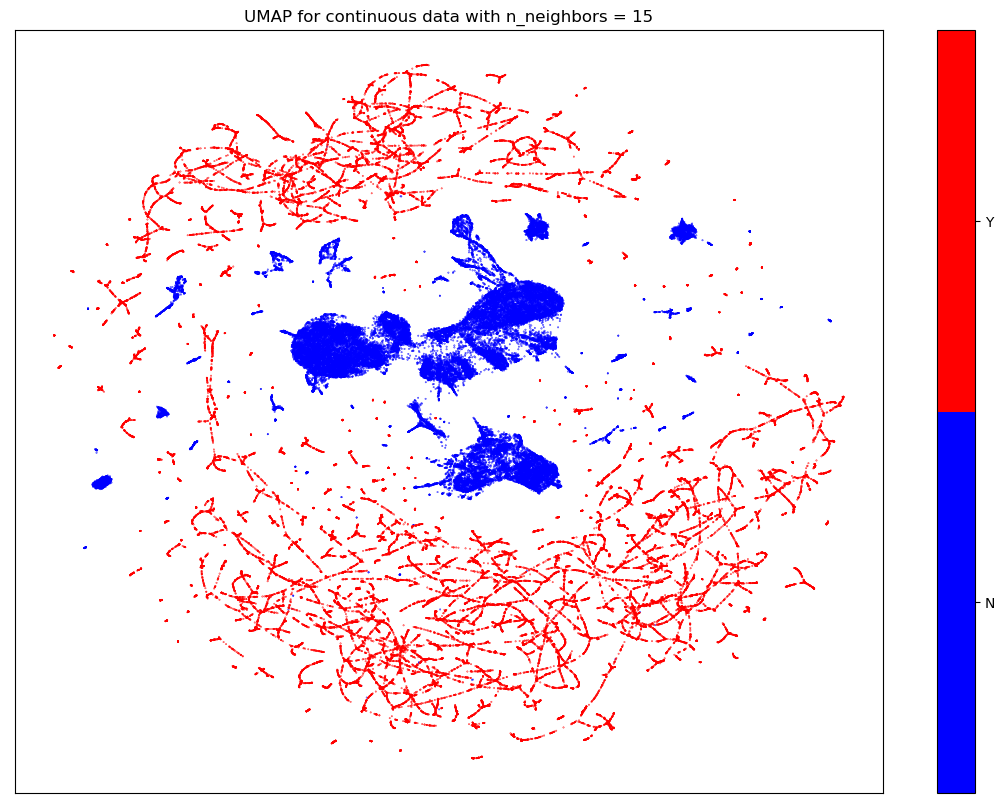
\includegraphics[width=1\linewidth]{umap_cont_n15}
  \caption{Continuous features}
  \label{fig:sub1}
\end{subfigure}%
\begin{subfigure}{.5\textwidth}
  \centering
  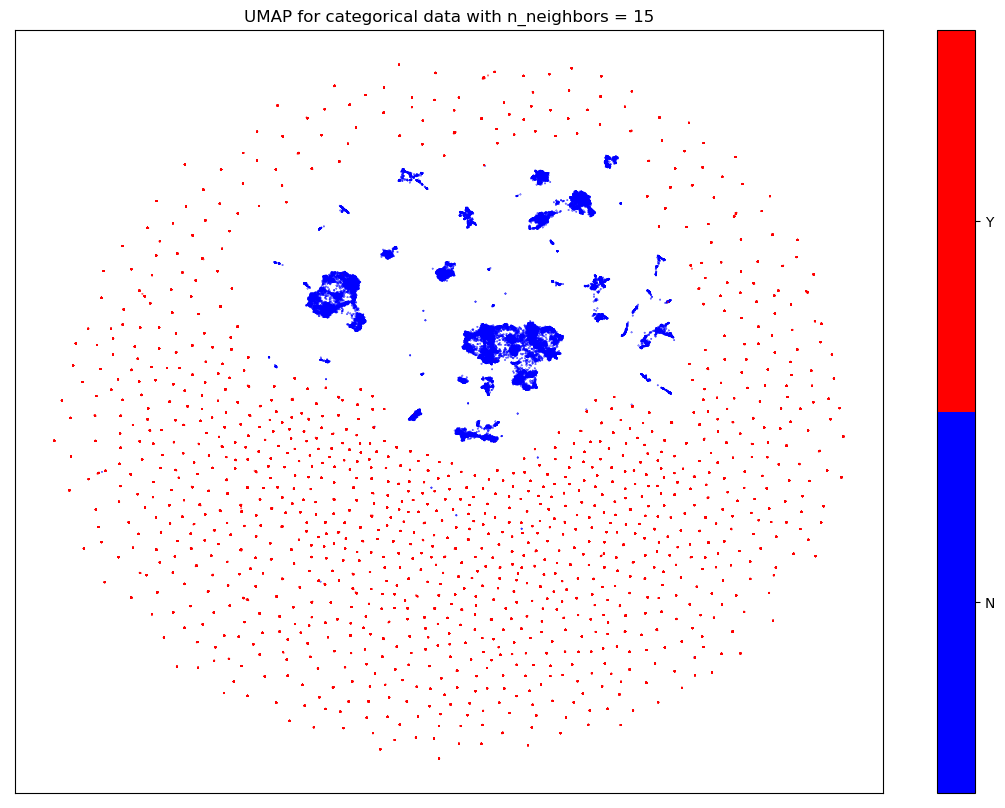
\includegraphics[width=1\linewidth]{umap_cat_n15}
  \caption{Categorical features}
  \label{fig:sub2}
\end{subfigure}
\caption{Visualization using supervised Umap, \texttt{n\_neighbors} = 15, \texttt{min\_dist} = 0.1, \texttt{n\_components} = 2}

\begin{subfigure}{.5\textwidth}
  \centering
  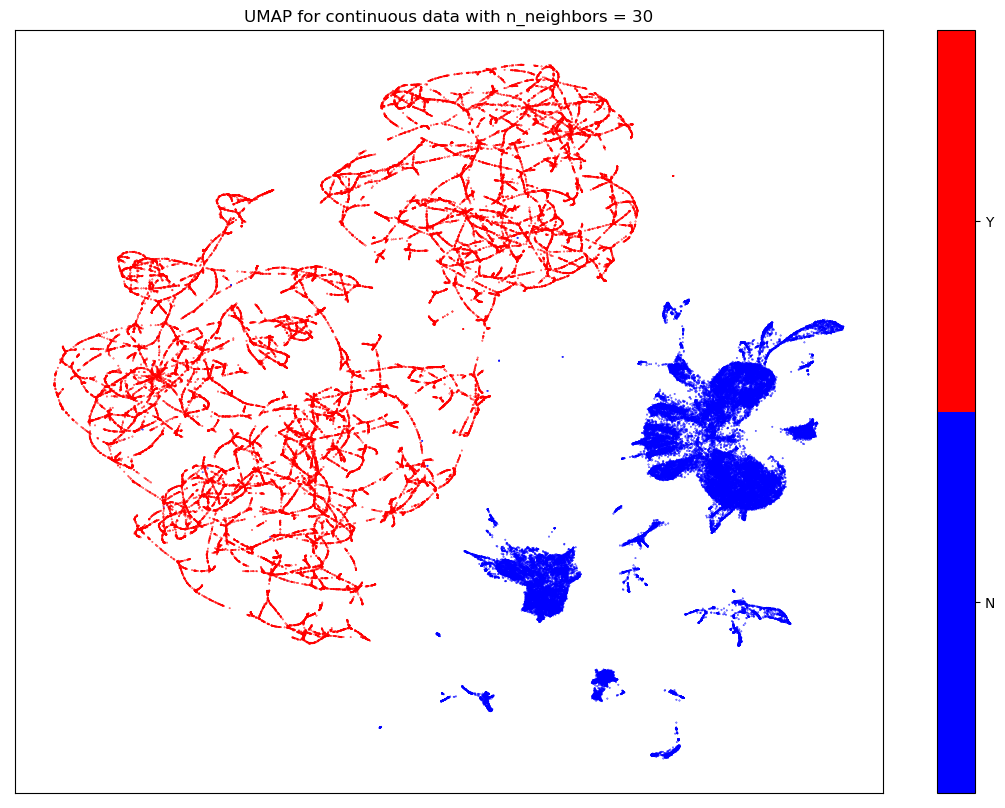
\includegraphics[width=1\linewidth]{umap_cont_n30}
  \caption{Continuous features}
  \label{fig:sub3}
\end{subfigure}%
\begin{subfigure}{.5\textwidth}
  \centering
  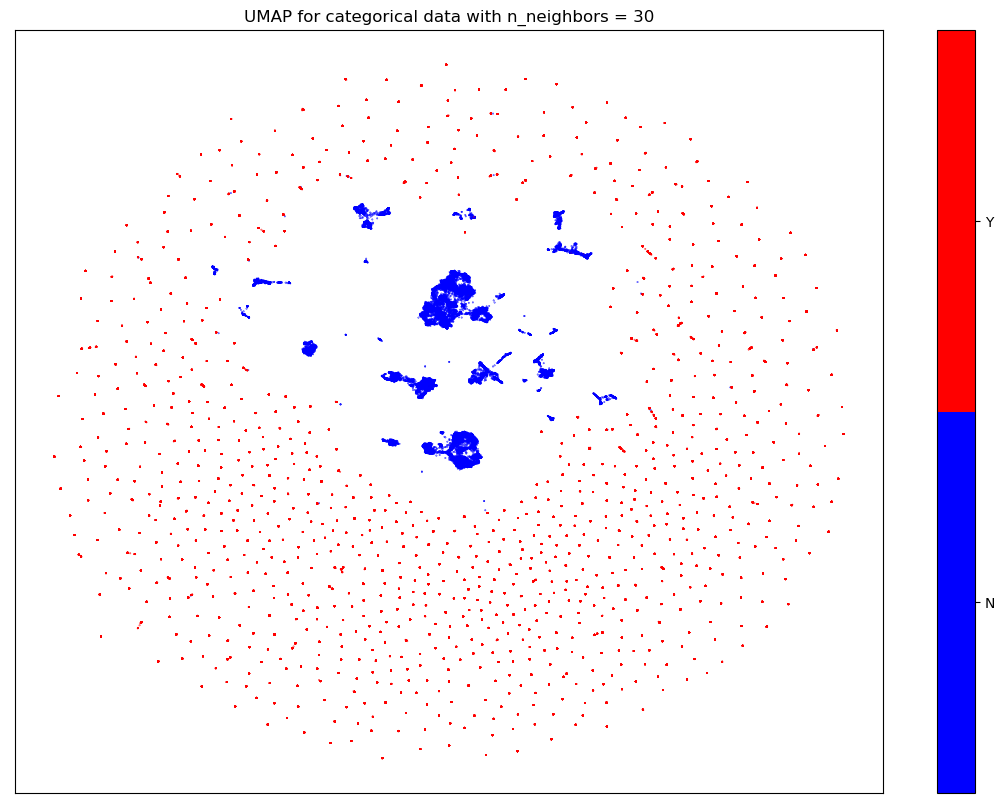
\includegraphics[width=1\linewidth]{umap_cat_n30}
  \caption{Categorical features}
  \label{fig:sub4}
\end{subfigure}
\caption{Visualization using supervised Umap, \texttt{n\_neighbors} = 30, \texttt{min\_dist} = 0.1, \texttt{n\_components} = 2}

\begin{subfigure}{.5\textwidth}
  \centering
  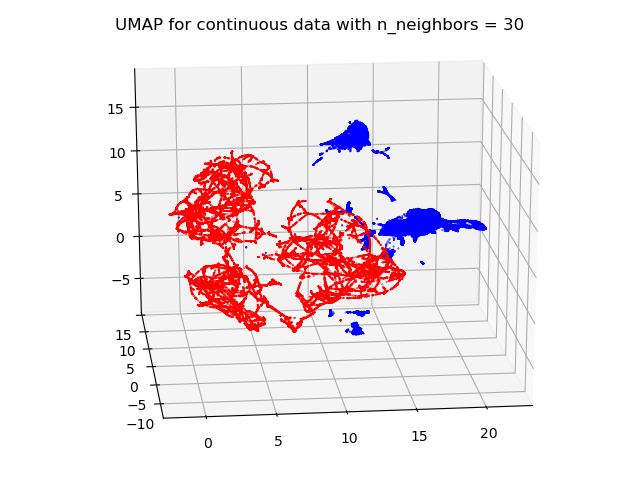
\includegraphics[width=1\linewidth]{umap_cont_3d}
  \caption{Continuous features}
  \label{fig:sub3}
\end{subfigure}%
\begin{subfigure}{.5\textwidth}
  \centering
  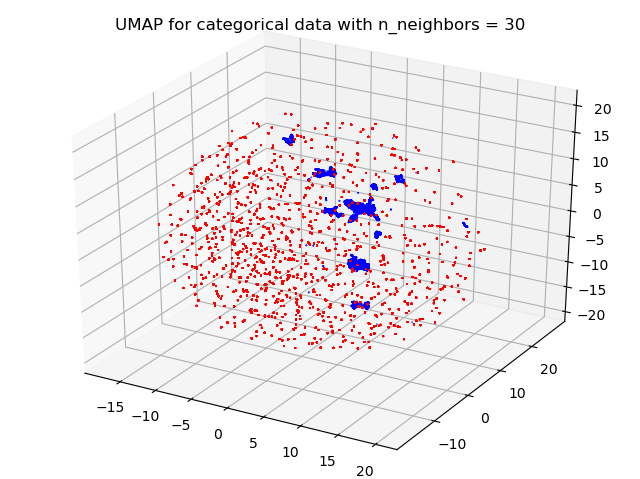
\includegraphics[width=1\linewidth]{umap_cat_3d}
  \caption{Categorical features}
  \label{fig:sub4}
\end{subfigure}
\caption{Visualization using supervised Umap, \texttt{n\_neighbors} = 30, \texttt{min\_dist} = 0.1, \texttt{n\_components} = 3}
\end{figure}

\clearpage
When the number of neighbourhood increases from 15 to 30, fraudulent cases are more connected to each other in the embedded representation for continuous features. So, it preserves more global structure of the training data. If we colour the output from Umap with the claim amounts, a weighting variable which is not included in training the Umap, we observe fraudulent cases with high claiming amounts are staying closer to each other in Figure 22. Thus, Umap seems able to capture the topological structure of fraudulent cases with high claiming amount. This pattern is less clear for categorical features but it also depends on the distance metric for categorical features.\\

Ideally, we can construct a weighted Umap model combining both Umap models for both continuous and categorical features. However, it may introduce extra hyperparameters to tune which make the training process much complicated. For example, we may need to tune the weighting parameter which assign weights to both models. Moreover, it will make the training process much time-consuming because the combined model also requires optimization. However, it can give us a more holistic view on the training data.

\begin{figure}[h]
\centering
\begin{subfigure}{.5\textwidth}
  \centering
  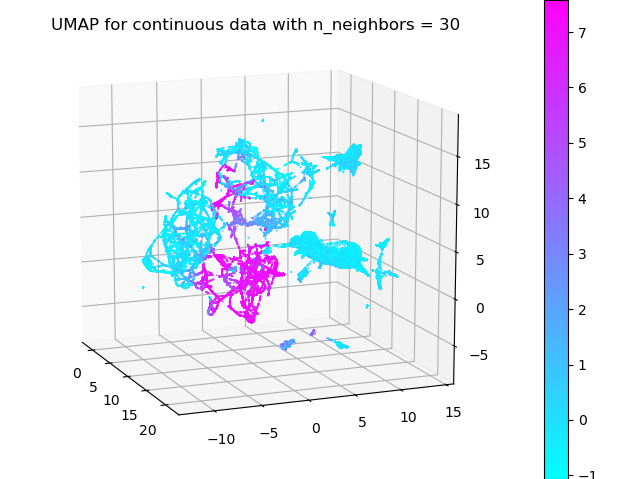
\includegraphics[width=1\linewidth]{umap_cont_3d_claim_amount}
  \caption{Continuous features}
  \label{fig:sub1}
\end{subfigure}%
\begin{subfigure}{.5\textwidth}
  \centering
  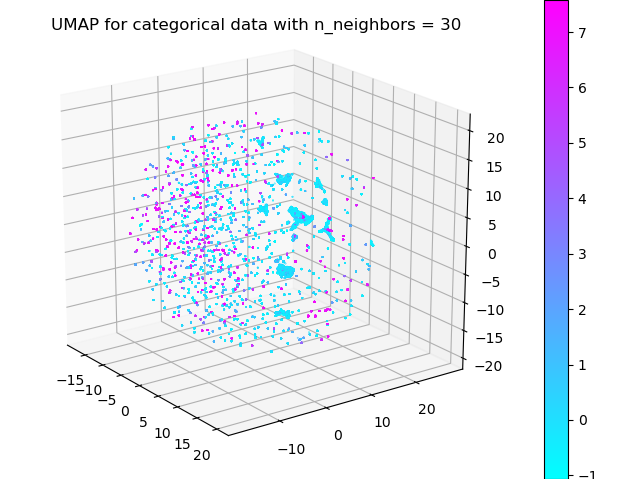
\includegraphics[width=1\linewidth]{umap_cat_3d_claim_amount}
  \caption{Categorical features}
  \label{fig:sub2}
\end{subfigure}
\caption{Visualization of Umap output in figure 20 coloured by \texttt{claim\_amount}}

\begin{subfigure}{.5\textwidth}
  \centering
  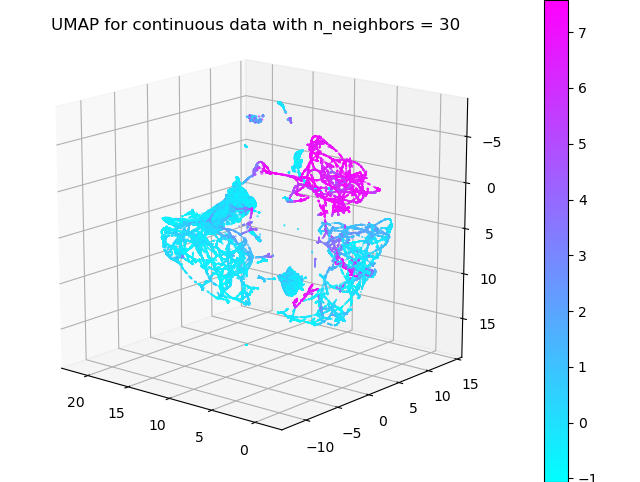
\includegraphics[width=1\linewidth]{umap_cont_3d_claim_amount_rotated}
  \caption{Continuous features}
  \label{fig:sub3}
\end{subfigure}%
\begin{subfigure}{.5\textwidth}
  \centering
  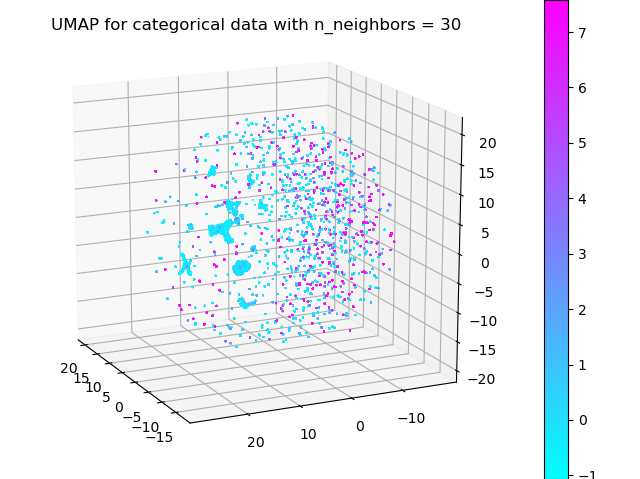
\includegraphics[width=1\linewidth]{umap_cat_3d_claim_amount_rotated}
  \caption{Categorical features}
  \label{fig:sub4}
\end{subfigure}
\caption{Rotated version of figure 21}
\end{figure}

\subsubsection*{Outlier detection}
\addcontentsline{toc}{subsubsection}{Outlier detection}

In this section, we apply outlier detection algorithm to the training dataset so as to find out extreme observations. In particular, we are also interested if extreme observations are associated with higher claiming amounts and fraudulent claims. It is possible to perform outlier detection using boxplot for each continuous features. However, it does not necessarily reflect an outlier in a higher dimensional space. In contrast to other popular outlier detection algorithms, isolation forest has much fewer hyperparameters to tuned when compared to one-class support vector machine and does not require distance metric like local outlier factor method. As scikit learn does not support Gower's distance in local outlier factor method, isolation forest becomes a more appealing tool. We use isolation forest from \texttt{sklearn.ensemble}, and it can assign anomaly scores based on the number of partitions needed to isolate an observation. Anomaly scores are further analyzed with other features, for example, \texttt{claim\_amount} and \texttt{fraud}. \\

In figure 23, we observe that fraudulent cases do not have anomaly scores higher than non-fraudulent cases. There is no obvious pattern between the anomaly scores and their claim amounts as well. So, observations with higher anomaly scores do not necessarily have higher claim amounts. In fact, the median of anomaly scores for fraudulent cases is lower than that for non-fraudulent cases.

\begin{figure}[h]
\centering
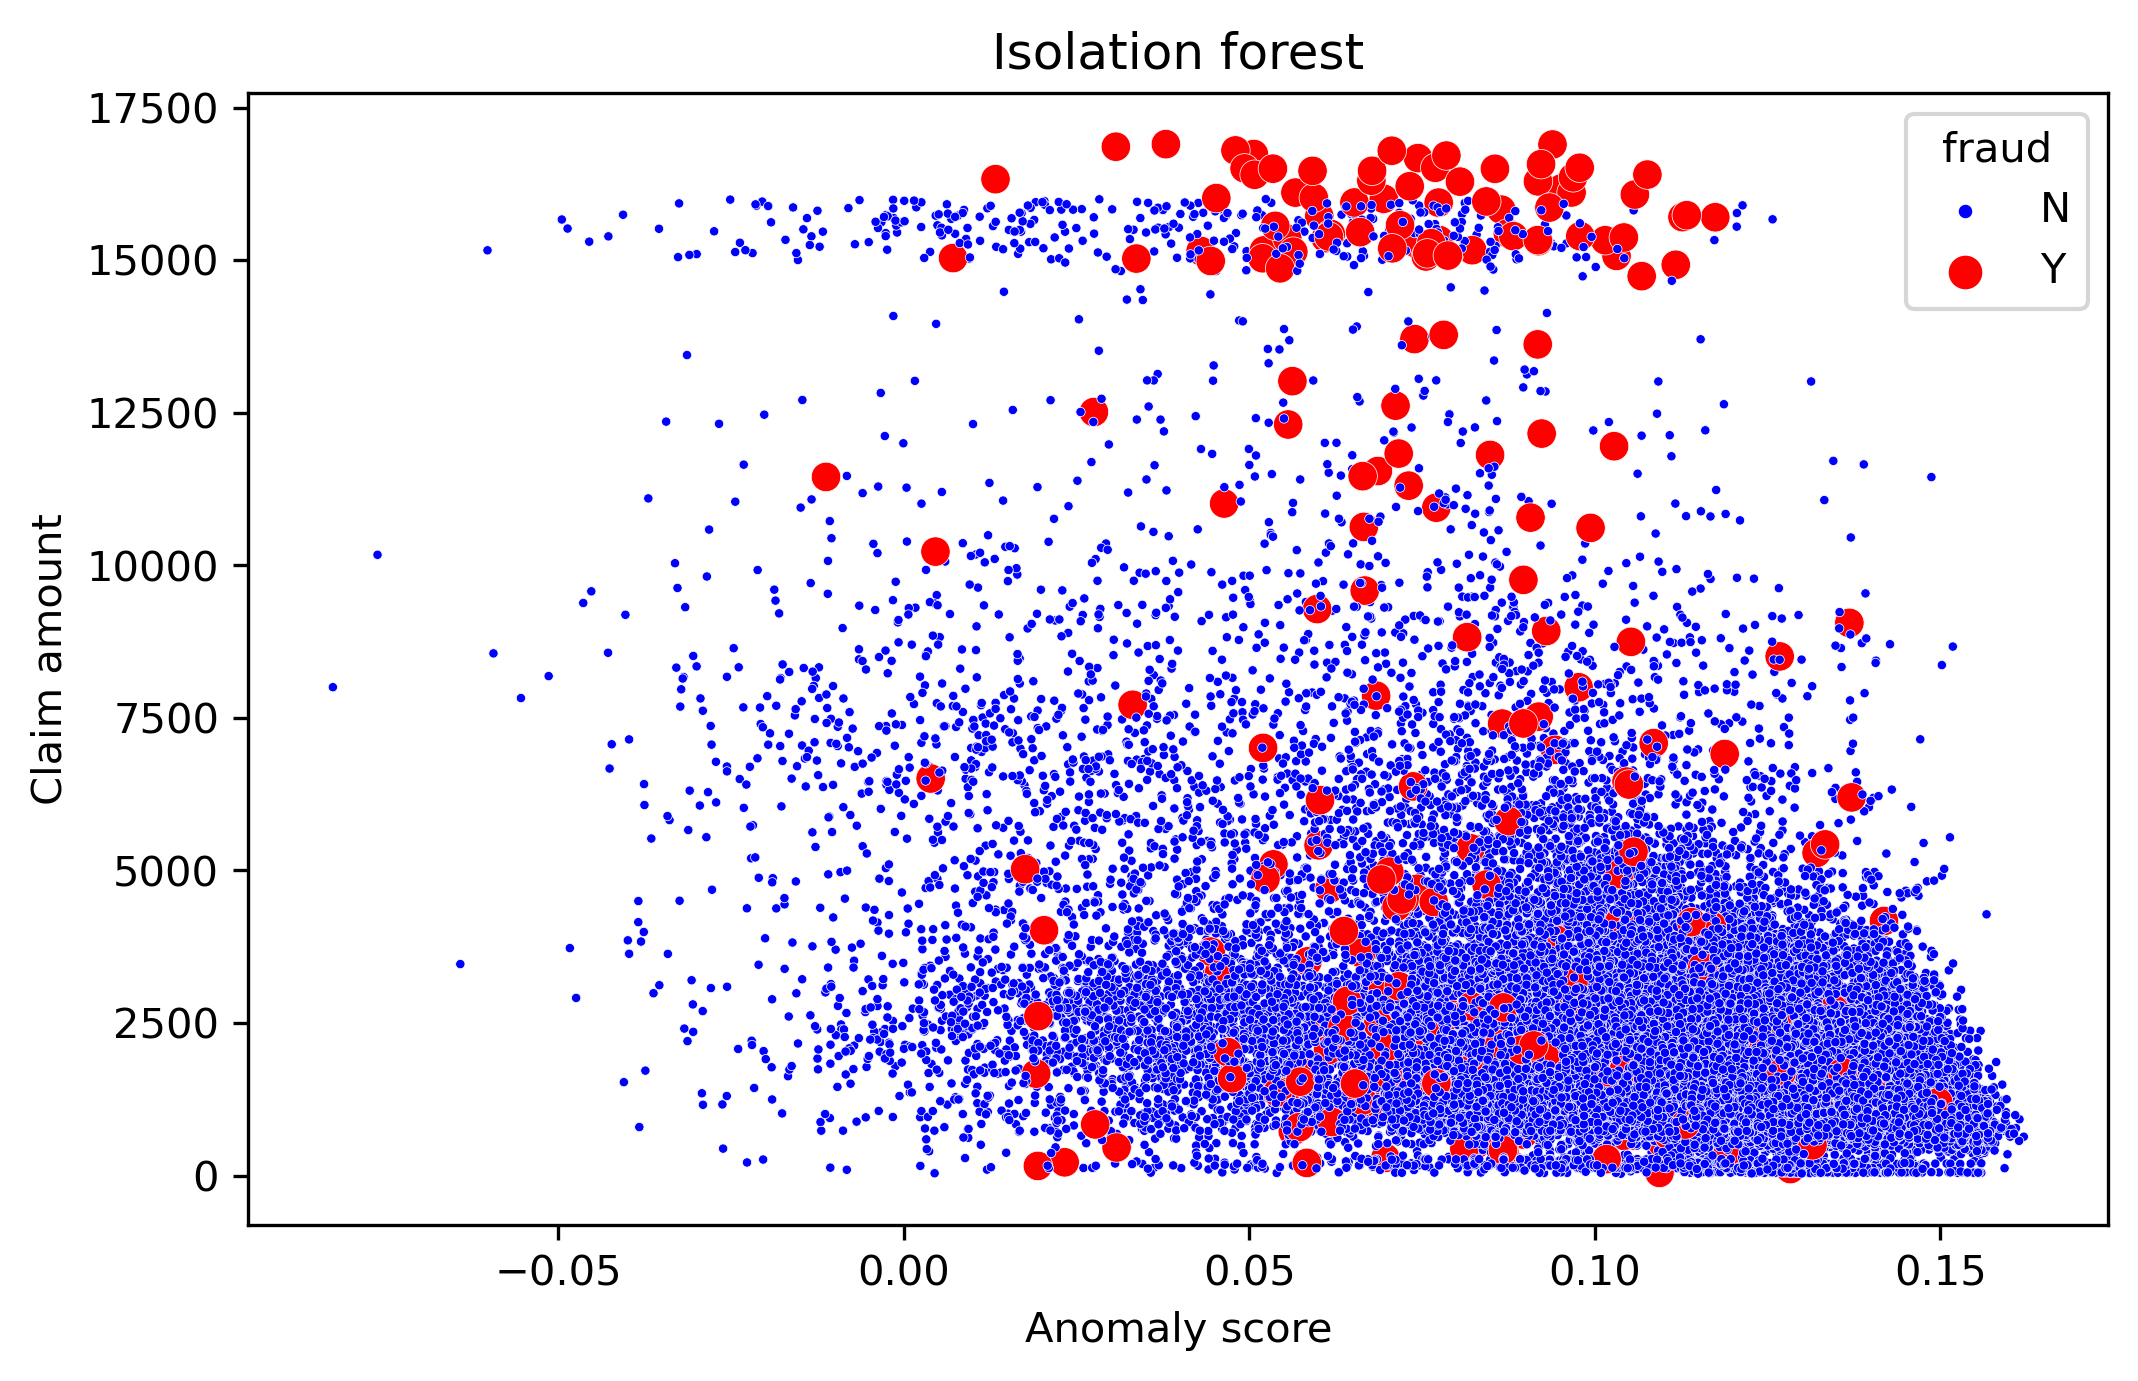
\includegraphics[width = 11cm, height = 8cm]{isolation_forest_results}
\caption{Joint distribution of anomaly scores estimated by isolation forest and their claim amounts}
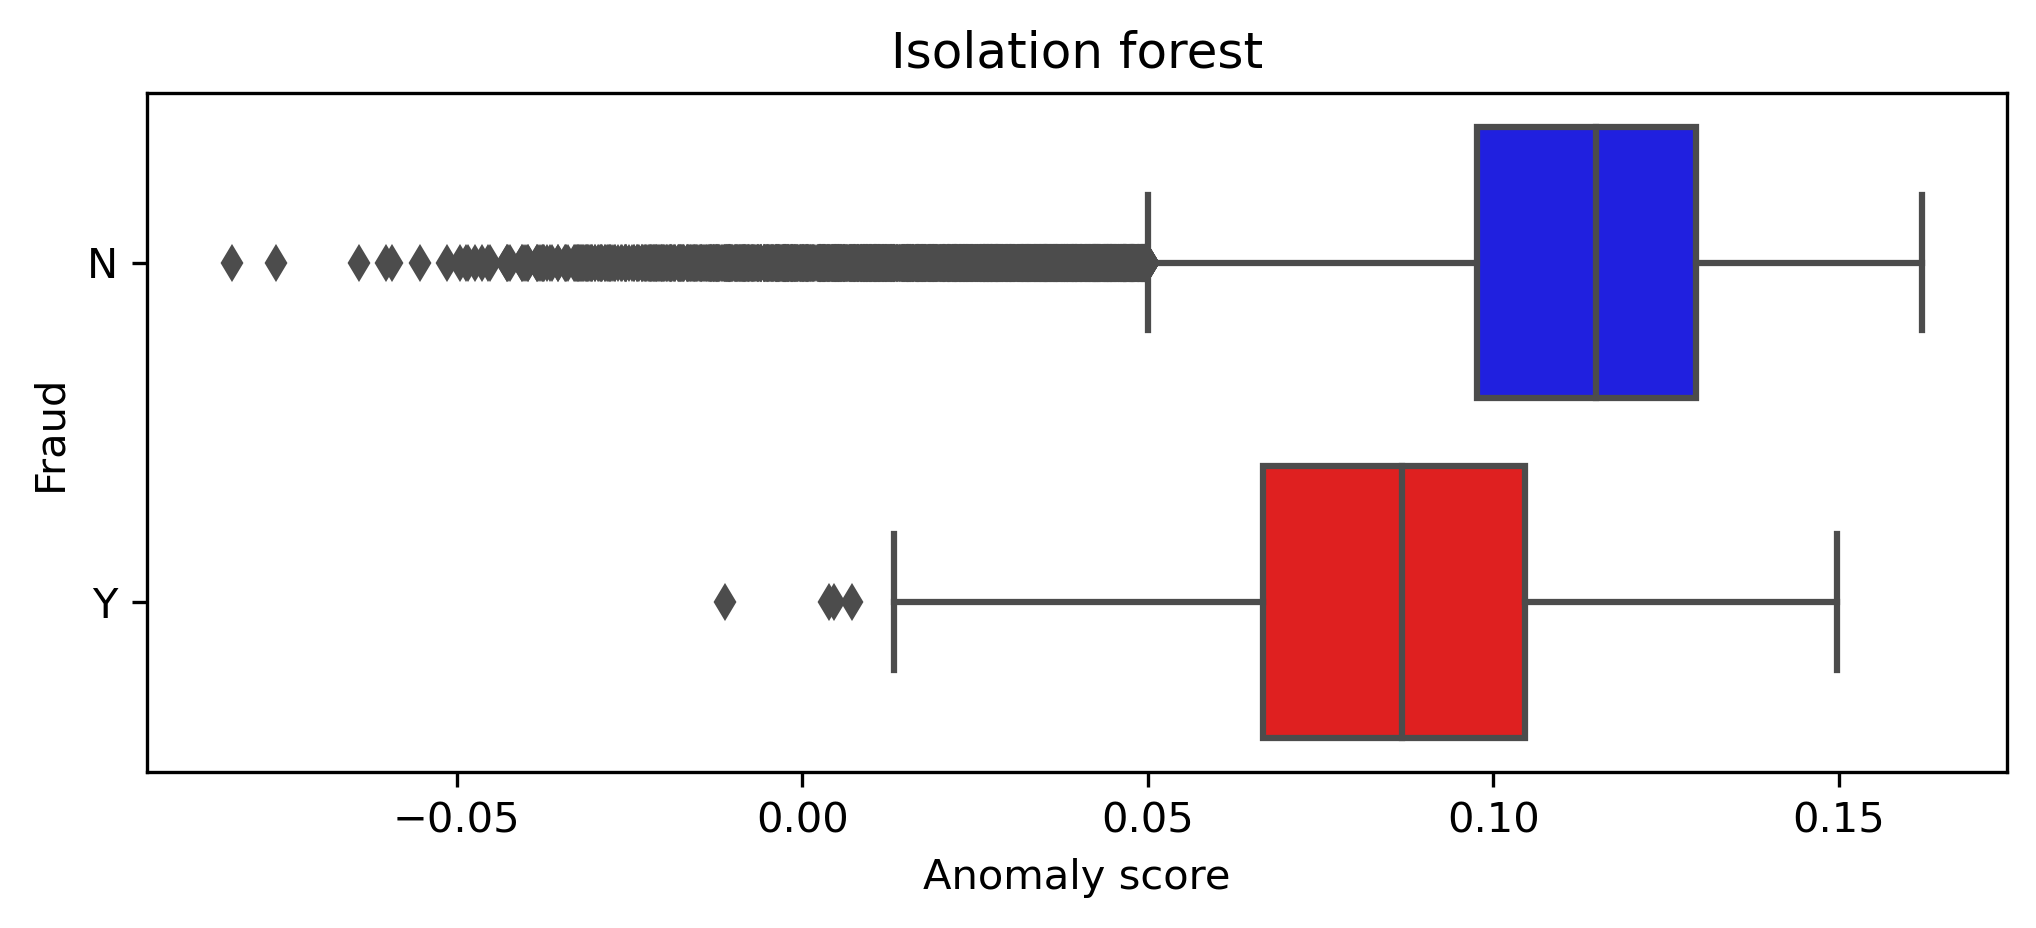
\includegraphics[width = 11cm, height = 5cm]{isolation_forest_results2}
\caption{Distribution of anomaly scores by fraudulent status}
\end{figure}

\clearpage
\subsection*{Model building}
\addcontentsline{toc}{subsection}{Model building}

The goal of this task is to predict top 100 fraudulent claims in terms of their claim amounts. In this section, we outline our model building process and justify how our choices are made.

\subsubsection*{Algorithms}
\addcontentsline{toc}{subsubsection}{Algorithms}

In this subsection, we summarize the motivations, packages and hyperparameters of the algorithms in the model building process.\\

As our training data contains missing values for many features. Unlike categorical features, missing values in continuous features require imputation because it cannot be grouped as an extra factor level. There are several popular imputation techniques, including mean, median, mode imputations in \texttt{SimpleImputer} and kNN imputation in \texttt{KNNImputer} from \texttt{sklearn}. Among mean, median and mode imputations, median imputation is the best choice because mean imputation reduces feature variances and mode imputation may not be suitable for continuous features which usually has distinct values. Compared to median imputation, kNN imputer is a better choice because different values are assigned based on its neighbourhood. During the training process, we discovered kNN imputer lengthens the training time by a lot in cross validation for grid search and probability calibration. Taking training time into account, we apply median imputer in the model.\\

As discussed in the section of exploratory data analysis, the dataset is highly imbalanced which requires sampling so that the classification becomes feasible. Otherwise, the classifier tends to lend the features of the majority class. As there are only 308 fraudulent cases, undersampling would lead to insufficient sample size in the training process. For oversampling, replication of observations form the minority class may encourage overfitting of the algorithm because the same patterns appear many time. Therefore, we need smart sampling technique which introduces some variability during sampling and reduce the risk of overfitting. For the task, we apply synthetic minority oversampling technique (SMOTE) which is available in \texttt{imblearn} library.\\ 


SMOTE is an algorithm which combines both oversampling and k nearest neighbourhood (kNN). For the minority class, the features of new sample are synthesized based on the k nearest neighbourhood of the observations from the minority class. Therefore, we need to tune the parameter $k$ for the number of nearest neighbourhood in kNN. We consider $k$ from 3 to 9.\\

For classifier, we focus on ensemble methods, and we use random forest, which is a classical and well-known ensemble method, as our baseline classifier, implemented in \texttt{sklearn} as \texttt{RandomForestClassifier}. Random forest requires only very few hyperparameters and is more robust to overfitting because the final prediction is calculated by the majority voting of individual decision trees. Some important hyperparameters in random forest are the maximum number of features used in constructing individual trees and the total number of such individual trees. We consider the maximum number of features from 10 to 70. For the total number of individual trees, we just need to ensure that it is sufficient for averaging effect to take place (and hence reduce the risk of overfitting).\\

Apart from random forest, we consider one of the latest ensemble technique, light gradient boosting machine (LightGBM), which is released 5 years ago. It is an efficient algorithm but comes with more than 100 hyperparameters, available in python as \texttt{lightgbm}. The details of all available hyperparameters can be found at \url{https://lightgbm.readthedocs.io/en/latest/Parameters.html}. LightGBM trains weak learners and grows the tree in a leaf-wise manner. LightGBM has a higher performance and efficiency but can be prone to overfitting. We consider the following hyperparameters in training LightGBM, learning rate in gradient boosting and the number of leaves for a weak learner. These hyperparameters are essential in balancing overfitting and predictive performance. We consider learning rate from 0.05 to 0.2 and the number of leaves from 10 to 30. We would compare its performance with a well-tuned random forest classifier, and further increase or reduce the search space of hyperparameters. 

\subsubsection*{Grid Search and Metrics}
\addcontentsline{toc}{subsubsection}{Metrics and Grid Search}

To tune the hyperparameters mentioned in the previous section, we need to perform a grid search over the hyperparameter space by cross validation. We prefer cross validation over train-validation set approach because using a single validation set can yield unstable performance metrics due to the randomness in splitting. Cross validation reduces the randomness by splitting the dataset into $k$ folds, and takes the average performance metrics. Moreover, each fold will be evaluated once in a $k$ folds cross validation. In contrast, some observations may never appear in the validation set even if train-validation set approach is done repeatedly. In this sense, cross validation is a better strategy in grid search.\\

However, it is highly possible that some folds do not contain any fraudulent cases due to class imbalance. 

\subsubsection*{Probability Calibration}
\addcontentsline{toc}{subsubsection}{Probability Calibration}



\subsubsection*{Data pipeline}
\addcontentsline{toc}{subsubsection}{Data pipeline}

\subsubsection*{Model Comparison}
\addcontentsline{toc}{subsubsection}{Model Comparison}


\subsection*{Interpretation}
\addcontentsline{toc}{subsection}{Interpretation}

\subsection*{Reflection}
\addcontentsline{toc}{subsection}{Reflection}

\clearpage
\section*{Assignment 2}
\addcontentsline{toc}{section}{Assignment 2}

\clearpage
\section*{Assignment 3}
\addcontentsline{toc}{section}{Assignment 3}

\clearpage
\section*{Assignment 4}
\addcontentsline{toc}{section}{Assignment 4}
\end{document}